\documentclass[uplatex, dvipdfmx]{jsarticle}
\usepackage{amsmath, amsthm, amssymb}
\usepackage{ascmac,here,txfonts,txfonts}
\usepackage[margin=2.5cm]{geometry}
\usepackage{color}
\usepackage{graphicx}
\usepackage{algorithm}
\usepackage{algorithmic}
\usepackage[subrefformat=parens]{subcaption}
\usepackage{hyperref}
\usepackage{csquotes}
\usepackage[backend=biber, style=numeric, sorting=none]{biblatex}
\usepackage[format=hang]{caption}

\captionsetup{compatibility=false}

\addbibresource{references.bib}

\setlength{\parindent}{0.3in}

\title{ Visualization of Kleinian Groups }
\author{ Kento Nakamura\\
Meiji University\\
}

\date{}

\pagestyle{headings}

\begin{document}

\maketitle

\begin{abstract}
 クライン群(\textit{Kleinian Groups})は数学の中でトポロジーや双曲幾何学に属する分
 野の一つである.クライン群は様々な方法で可視化することで,フラクタルと
 呼ばれる美しい幾何学的構造を見ることができる.
 筆者はクライン群をコンピュータで可視化することに焦点をおいて学習してきた.
 ここではクライン群の可視化手法とこれまでに研究されてきたクライン群に関す
 る話題の中でも,興味を引くような図像をみることができるものをまとめた.
 また,それらに付随して,その他のフラクタルの描画やテセレーション
 と呼ばれる敷き詰め模様の描画方法についてもまとめた.
 
 1章ではいくつかのフラクタルとそのレンダリング手法についてまとめる.
 ここで述べる手法は後でクライン群を効率よく描画するための基礎となる.
 2章ではクライン群の可視化手法とその周辺分野について記述する.
 3章ではテセレーションのレンダリング手法をまとめる.

 筆者が書いたプログラムの多くは\textit{GitHub}\footnote{GitHub:
 ~\url{https://github.com/soma-arc}}や
 \textit{Shadertoy}\footnote{Shadertoy:
 ~\url{https://www.shadertoy.com/user/soma\_arc}}で公開されている.
 また,講演スライドや論文は筆者のウェブページ
 \footnote{筆者のウェブページ: \url{https://knkmr.net}}で公開されている.

\end{abstract}

\clearpage

\tableofcontents

\clearpage

%#!uplatex main.tex

\section{Fractal}

\emph{フラクタル}(\textit{fractal})は数学者ブノワ・マンデルブロ(Benoit
B. Mandelbrot)が提唱した幾何学の概念である.フラクタル図形とよばれる図形
は自己相似性を持ち,図形のどこを拡大しても全体と同じ形を見ることができる.

図\ref{fig:gasket}に\emph{シェルピンスキーのギャスケッ
ト}(\textit{Sierpinski gasket})とよばれるフラクタル図形を示した.
三角形を一定の法則に基づいて分割していくことで得られる図形である.
図\ref{fig:menger}に示される物体は\emph{メンガーのスポンジ}(\textit{Menger
sponge})とよばれ,立方体に一定の法則で穴を空けることで得られる.
これらの形はどこを拡大しても同様の法則性を持った形をみることができる.

海岸線やシダ植物,体内の肺など自然界の多くの場所でもフラクタル構造をみる
ことができる.
フラクタルを考えることは自然科学研究の新たなアプローチとしても発展した.

フラクタルの特異な形状は多くの人々の興味を引き,アートとしても大きく発展
した.これにはコンピュータの普及も大きく関連しており,コンピュータ文化と
は切り離せない.
インターネット上のフラクタルコミュニティとして最大のものに,\textit{Fractal
Forum}\footnote{Fractal Forum:~\url{http://www.fractalforums.com/}}
という電子掲示板がある.
このコミュニティから生まれたフラクタル図形や描画手法はとても多い.

また,\emph{デモシーン}(\textit{Demoscene})という文化もフラクタルレンダリン
グと関連が深い.
デモシーンは\emph{デモ}(\textit{Demo})とよばれるリアルタイ
ムにコンピュータグラフィクスや音楽を生成するプログラムを見せ合うコンピュータサブ
カルチャーの一つである.美しいコンピュータグラフィクスをリアルタイムに,
さらに小さなサイズのプログラムで描画することを追求している.
フラクタルは形として面白いことに加え,数式で複雑な形状を描画できるの
でデモと相性がよい.

デモシーンに関しては\textit{Demoscene - The
Art of the Algorithm}\footnote{Demoscene - The Art of the Algorithms:
~\url{https://www.youtube.com/watch?v=iRkZcTg1JWU}}が詳しい.
また,著名なデモシーナーのInigo Quilez (iq)は自身のウェブページ\footnote{Inigo
Quilez's webpage:~\url{http://iquilezles.org/index.html}}にコンピュータグラフィ
クスに関する様々な記事をまとめている.
ここで紹介する手法もまとめられているので,併せて参考にされたい.

この章では,後のクライン群の可視化に関わりのあるフラクタルとその描画手
法についてまとめる.
ここで記述があるもの以外にも様々なフラクタルが存在している.
マンデルブロ自身の著作である『フラクタル幾何学』
\cite{mandelbrot-ja-201102-1}
\cite{mandelbrot-ja-201102-2}
(原著:~\cite{mandelbrot1983fractal})では種々のフラクタルが網羅的にまとめ
られている.

\begin{figure}[htbp]
 \begin{minipage}{0.5\hsize}
   \center
  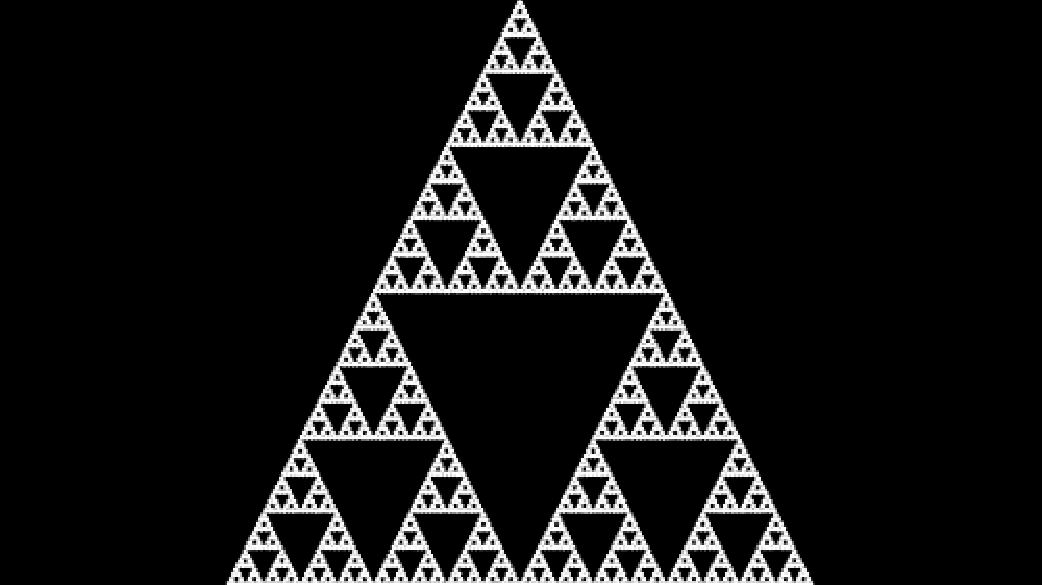
\includegraphics[width=3in, height=3in, keepaspectratio]{../img/fractal/gasket.pdf}
  \caption{Sierpinski gasket}
  \label{fig:gasket}
 \end{minipage}
 \begin{minipage}{0.5\hsize}
  \center
  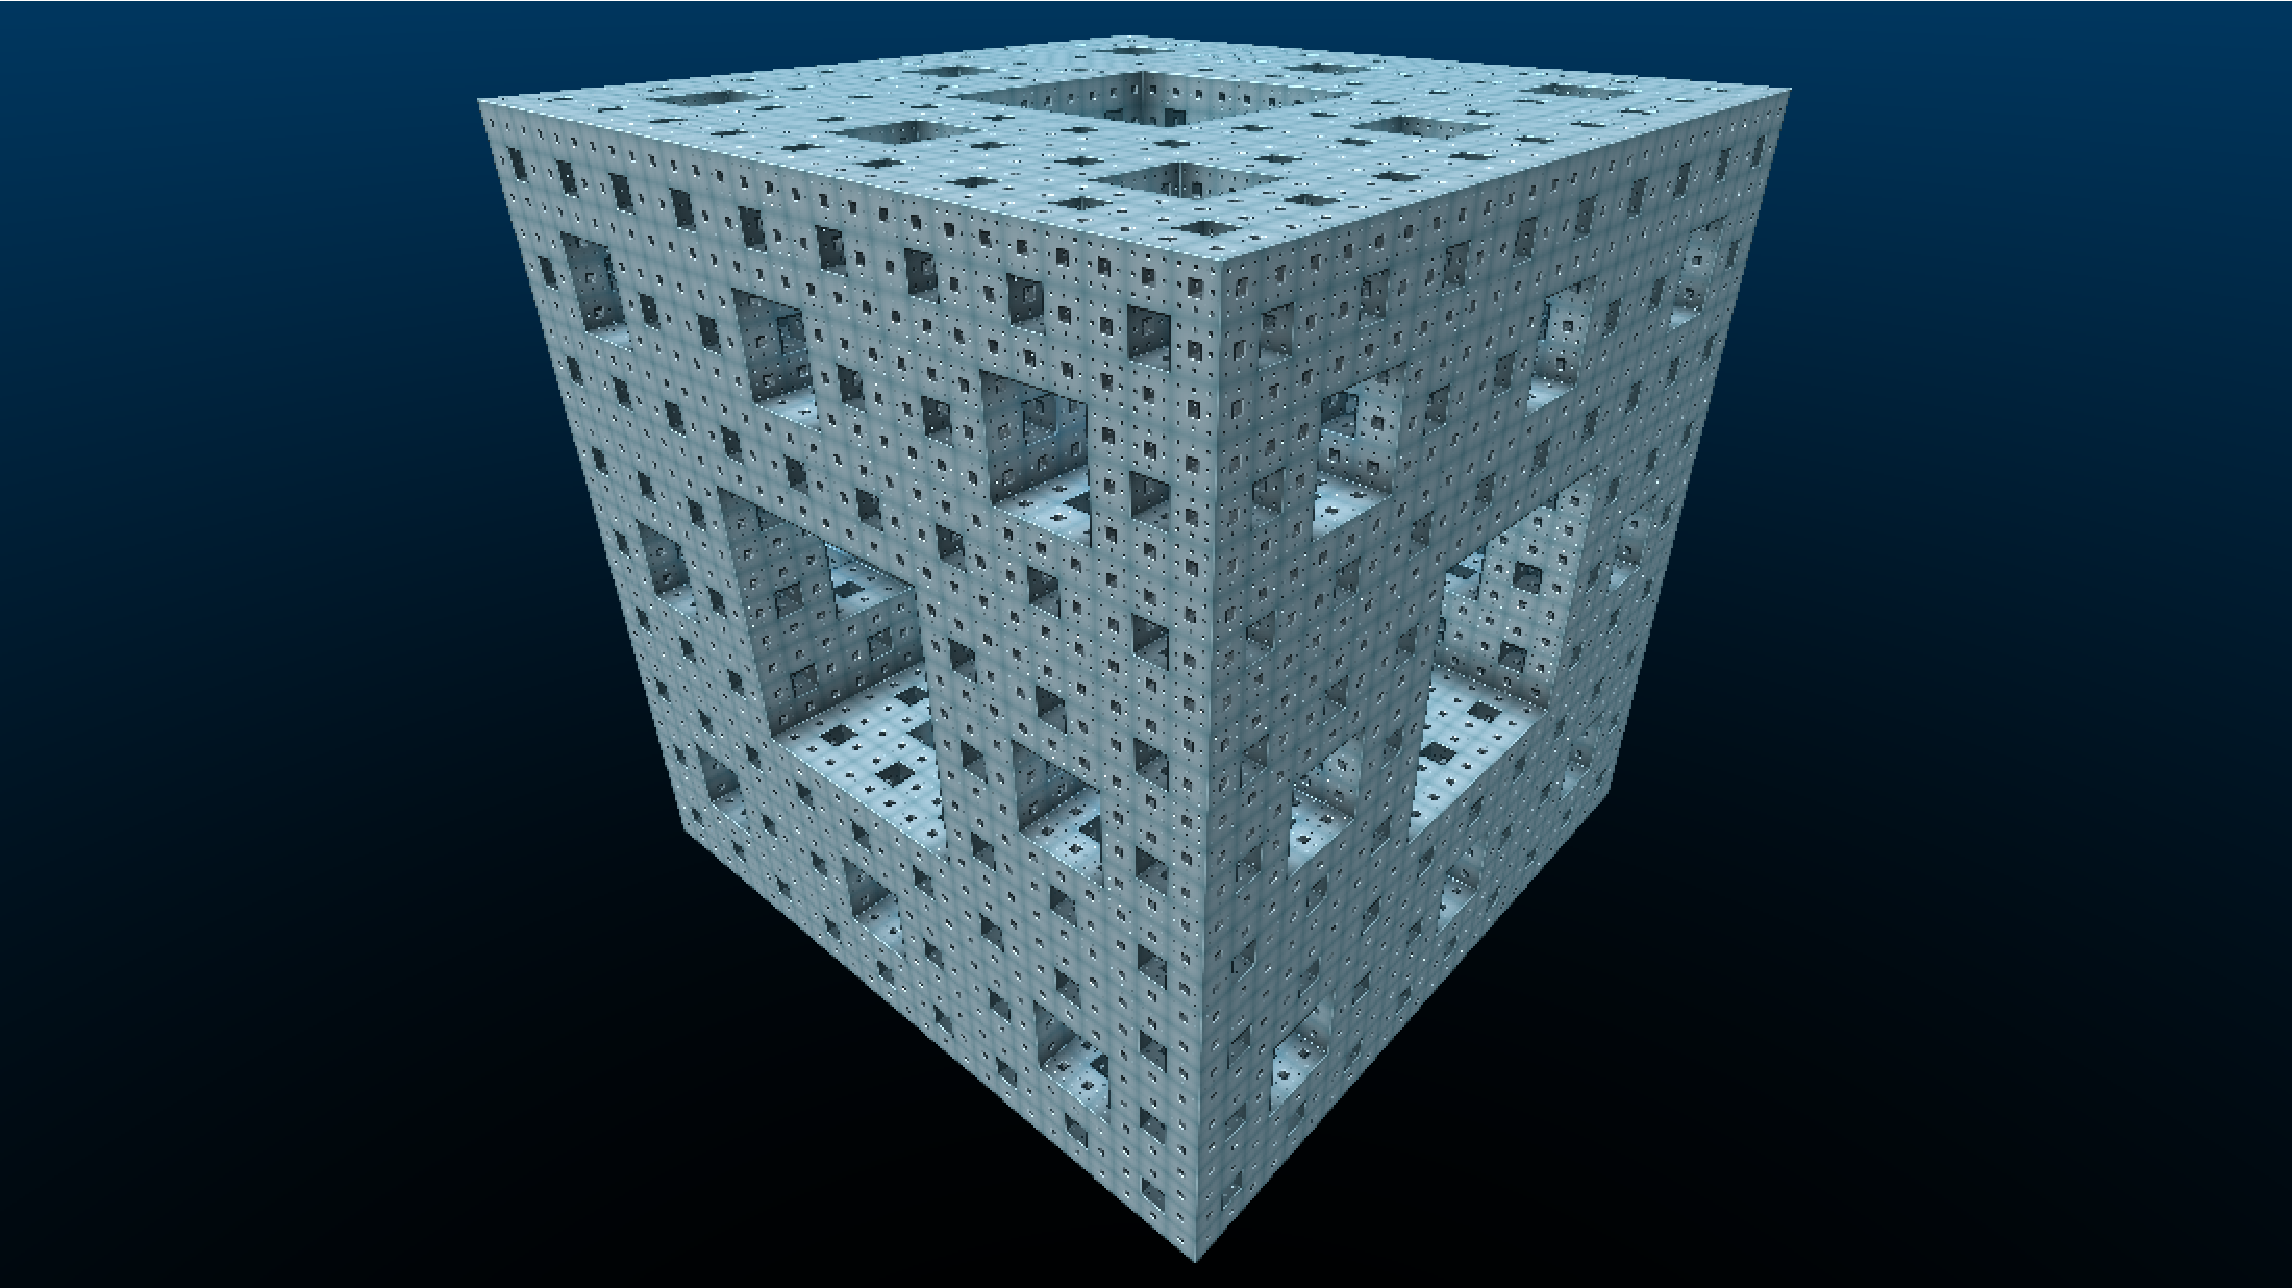
\includegraphics[width=3in, height=3in, keepaspectratio]{../img/fractal/menger.pdf}
  \caption{Menger sponge rendered with Fractal Lab}
  \label{fig:menger}
 \end{minipage}

\end{figure}

\subsection{Shader Based Rendering}

最近のデモ作品でよく用いられる作品制作手法の一つに\textit{OpenGL Shading
Language (GLSL)}や\textit{High Level Shading Language (HLSL)}の\emph{フラ
グメントシェーダ}(\textit{Fragment Shader})を用いるものがある.
フラグメントシェーダは本来,ポリゴンに陰影をつけるために使用され,その処
理はGPUで行なわれる.
GPUは浮動小数演算性能に優れていることに加え,各ピクセルの演算は並列に行
われるため高速である.

この手法はスクリーンスペースに矩形のポリゴンをレンダリングすることで
\emph{プロシージャル}(\textit{Procedural})に図を描画する.
プロシージャルとは数式やアルゴリズムを用いて形状を生成することを
指す.
複雑な形状をあらかじめモデリングされたポリゴンで表現するよりもプログラム
の実行サイズを下げたり,計算速度を向上させたりすることができる.
このことはデモにおける小さなプログラムサイズでリアルタイムにレンダリングする
という目的に適している.
フラクタルはしばしば簡潔なアルゴリズムで複雑な形状を生成するので,デモに
おいてもよく使われる.

シェーダはピクセルごとにその座標とCPU側から渡される変数を受け取る.
これらを用いてピクセルの色を決定する.
アルゴリズム\ref{shaderSample}に座標から色を決定して塗るシェーダの
擬似コードを示した.
図\ref{fig:simpleShader}にそのレンダリング結果を示した.
\begin{algorithm}
 \begin{algorithmic}
  \begin{minipage}{0.5\hsize}
   \caption{Sample shader}
   \label{shaderSample}
   \REQUIRE COORDINATES, resolution
   \STATE uv $\leftarrow$ COORDINATES / resolution
   \STATE COLOR $\leftarrow$ Vector3(uv.x$,~$uv.y$,~1$)
  \end{minipage}
 \end{algorithmic}
\end{algorithm}

幾何図形を描く際には\emph{距離関数}(\textit{Distance Function})がよく用いられる.
距離関数は任意の点が与えられたときに,その点と図形の最短距離を返す関数である.
例えば,平面上の点$z$が与えられたとき,原点を中心とする半径$r$の円との距
離を返す距離関数$f(z)$は次のようになる.
\begin{align*}
 f(z) =  length(z) - r
\end{align*}
この関数は円周からの距離を返す.
そのため,平面上の各点に距離関数を作用させ,得られた距離が負であるときに
色をつける処理をシェーダで書くと円を描くことができる.
複数の図形を描きたい時は,複数の距離関数を評価し,最も小さな距離を求めれ
ばよい.
距離関数による描画は,得られた距離によって色の濃さを変えるといった工夫で
図形をより滑らかに描くことができる.
アルゴリズム\ref{renderCircle}に円を描く疑似コードを示した.図
\ref{fig:circleShader}にそのレンダリング結果を示した.

\begin{algorithm}
 \begin{algorithmic}
  \caption{Render circle}
  \label{renderCircle}
  \REQUIRE COORDINATES, resolution, radius
  \STATE p $\leftarrow$ COORDINATES $-$ (resolution$ / 2$)
  \STATE distance $\leftarrow$ length(p) $-$ radius
  \IF{distance $\leq$ 0}
  \STATE COLOR $\leftarrow$ Vector3($1,~1,~1$)
  \ELSE
  \STATE COLOR $\leftarrow$ Vector3($0,~0,~0$)
  \ENDIF
 \end{algorithmic}
\end{algorithm}

 \begin{figure}[htbp]
  \begin{minipage}{0.5\hsize}
   \center
   
\includegraphics[ height=1.5in, keepaspectratio]{../img/fractal/uv.pdf}
   \caption{Simple shader}
   \label{fig:simpleShader}
  \end{minipage}
  \begin{minipage}{0.5\hsize}
   \center
   
\includegraphics[ height=1.5in, keepaspectratio]{../img/fractal/circle.pdf}
   \caption{Circle}
   \label{fig:circleShader}
  \end{minipage}
 \end{figure}

シェーダを用いたレンダリングはglslsandbox\footnote{glslsandbox:
~\url{http://glslsandbox.com/}}やShadertoy\footnote{Shadertoy:
~\url{https://www.shadertoy.com/}}といったウェブサービスで手軽に試すこと
ができる.h\_doxasによるwgld\footnote{wgld:
~\url{https://wgld.org/d/glsl/}}にはシェーダによるレンダリングの入門事項
がよくまとまっている.

また,GPUの計算性能をより汎用的な計算に用いるためのプラットフォームとしてCUDA
やOpenCLが登場している.
これらのプラットフォームを用いることでシェーダではできない複雑な処理を
GPUで行うことができるようになり,GPUによる並列演算は機械学習などの分野に
も活躍の場を広げた.
このようにGPUによる演算を画像処理以外の汎用的な用途に用いる技術は
\textit{GPGPU (General-purpose computing on graphics processing units)}
とよばれている.

\subsubsection{Distance Estimation}

簡単な幾何図形の距離関数は簡単に導出できるが,そうでない図形やフラクタル
の場合は難しい.
しかし,\textit{Distance Estimation}という手法を用いることで,
距離関数を陰関数から近似的に導出することができる.
その式の一つをiqによる導出\footnote{distance estimation:
~\url{http://iquilezles.org/www/articles/distance/distance.htm}}
をベースにして紹介する.

図\ref{fig:distance-estimate}における赤色の曲線を表す陰関数$f(x)$を考え
る.
平面上のある点を$x$とし,陰関数が表す零点集合上で$x$から最も近い点を
$x + e$とすると,$e$は$x$から最も近い点へ向かうベクトルである.
そして求めたい距離は$|e|$となる.
 \begin{figure}[htbp]
  \center
  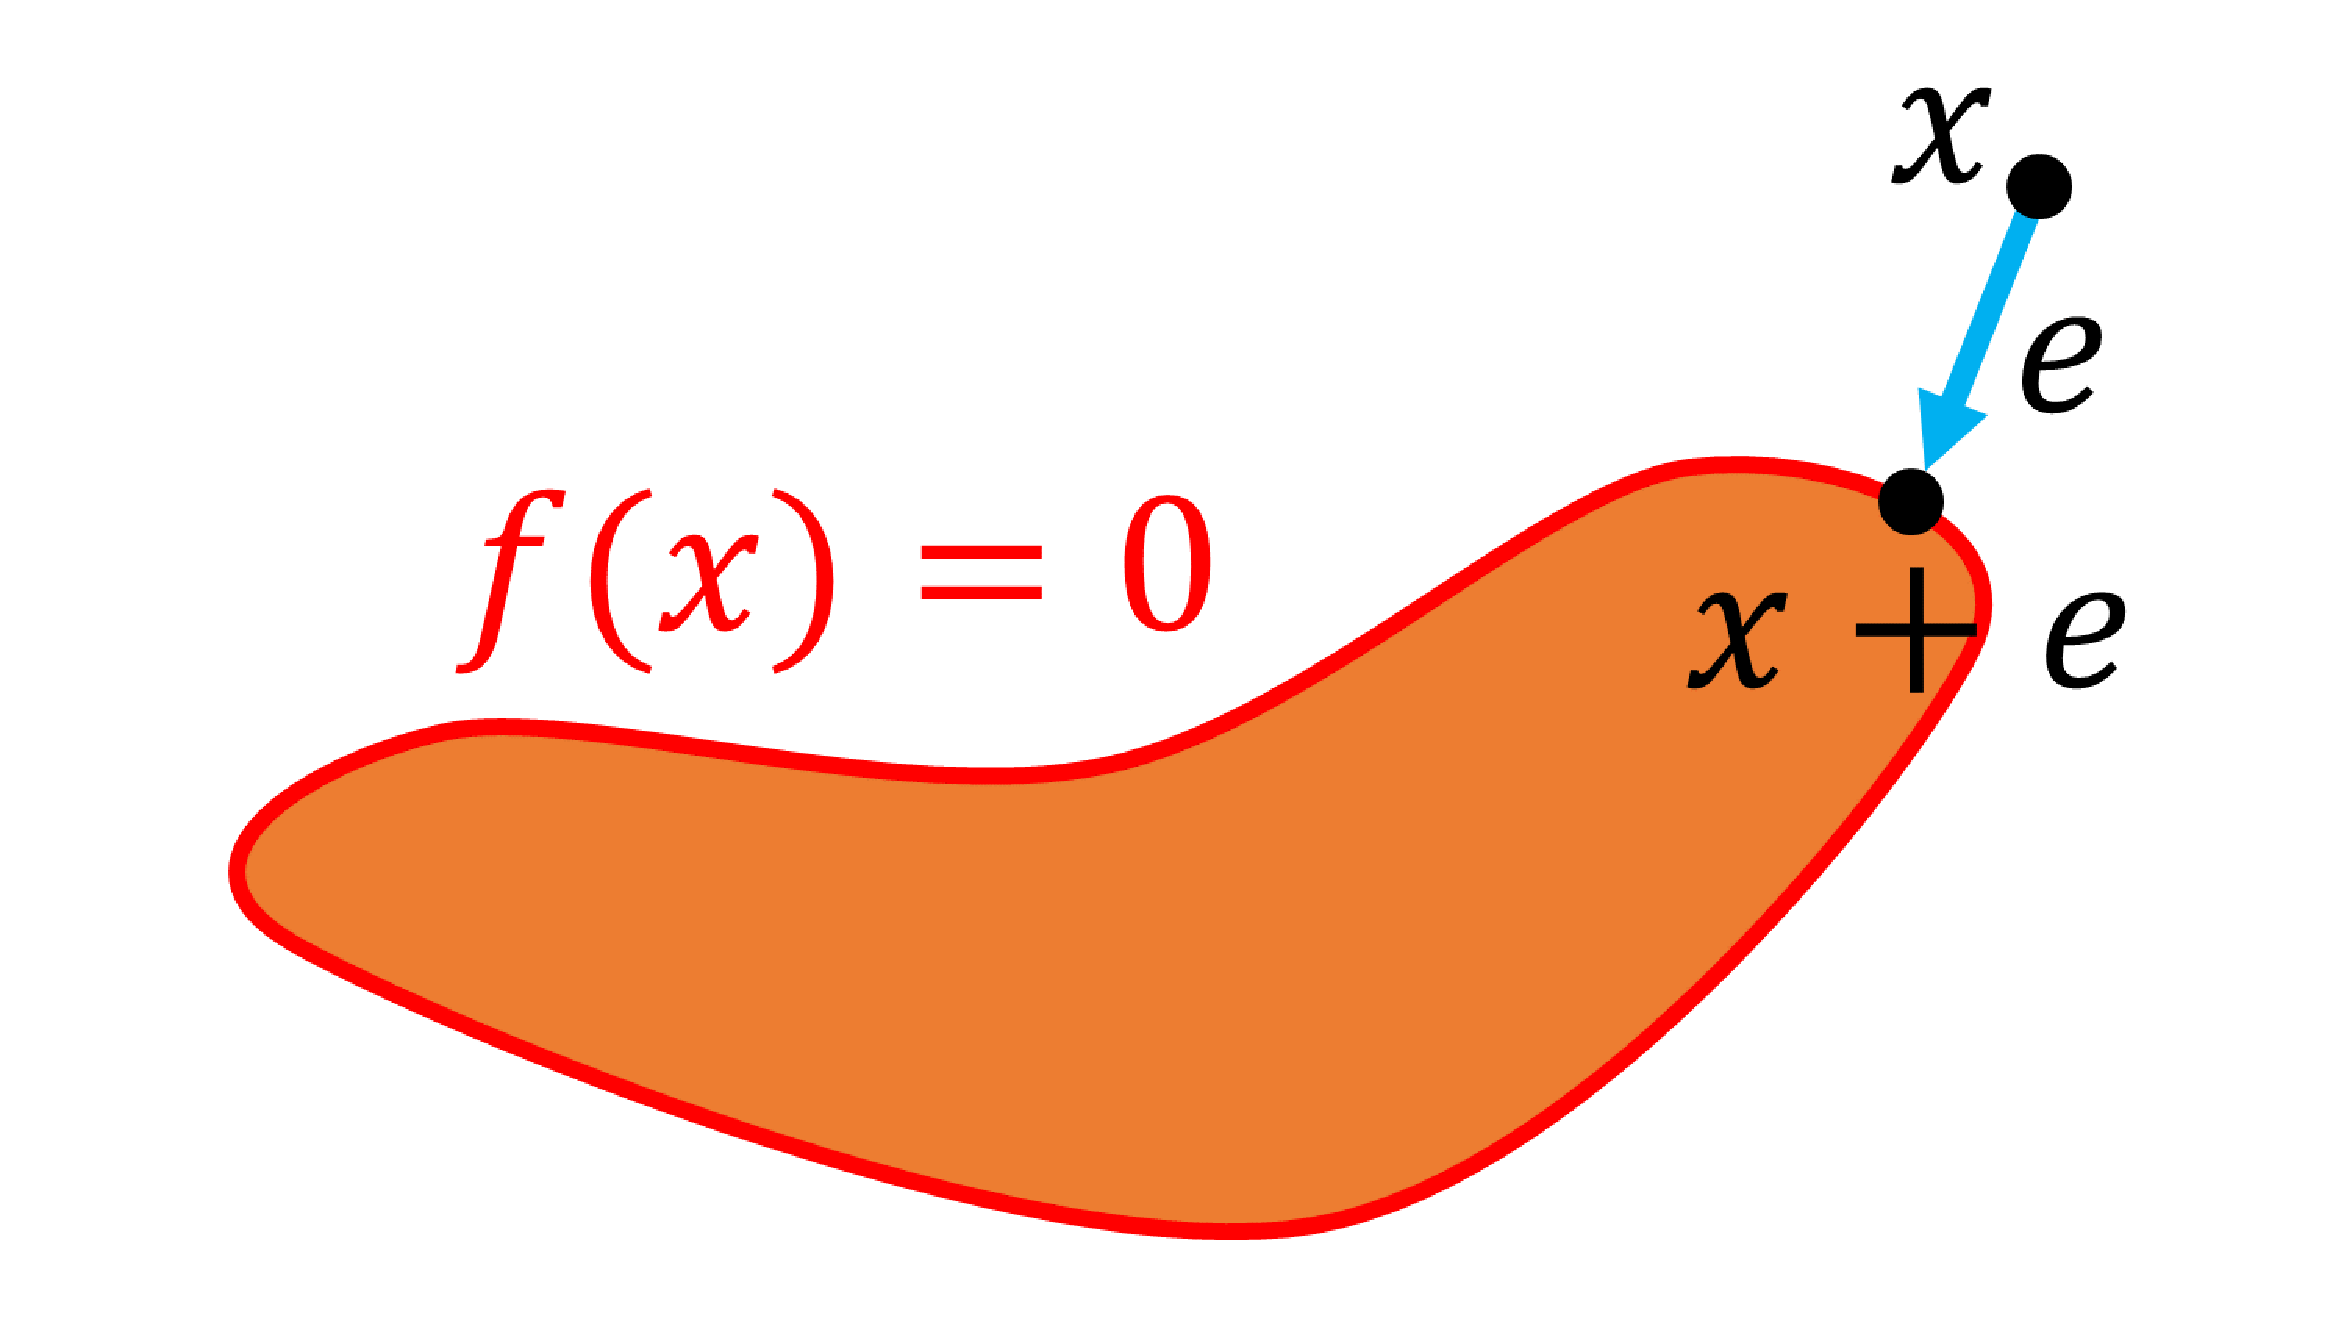
\includegraphics[width=3in, keepaspectratio]{../img/fractal/distance-estimate.pdf}
  \caption{Distance Estimation}
  \label{fig:distance-estimate}
 \end{figure}

$f(x + e) = 0$をテイラー展開すると次のようになる.
\begin{align*}
f(x + e) = f(x) + f'(x) \cdot e  + \frac{1}{2}f''(x) \cdot e^2 ...
\end{align*}
ここで$e$が十分に小さいと仮定し,2次以上の項を無視する線型近似を行うこと
で次の近似式を得る.
\begin{align*}
0=|f(x + e)| \approx |f(x) + f'(x) \cdot e|
\end{align*}
ここで,$x,~e$はベクトルであり$\cdot$は内積を表すことに注意する.
三角不等式によって,
\begin{align*}
| f(x) + f'(x) \cdot e| \geq |f(x)| - |f'(x) \cdot e|
\end{align*}
であるから,
\begin{align*}
0 \geq |f(x)| - |f'(x) \cdot e|
\end{align*}
となる.
次に,コーシーシュワルツの不等式より,
\begin{align*}
 |f'(x)| \cdot |e| \geq | f'(x)\cdot e|
\end{align*}
であるから,
\begin{align*}
 0 \geq |f(x)| - |f'(x) \cdot e| \geq |f(x)| - |f'(x)| \cdot |e|
\end{align*}
となる.
最後に
\begin{align*}
0 \geq |f(x)| - |f'(x)| \cdot |e|
\end{align*}
を変形すると
\begin{align*}
|e| \geq \frac{|f(x)|}{|f'(x)|}
\end{align*}
が得られる.
このことから,ある点$x$に対して陰関数$f(x)$が表す零点集合への最短距離を返す近
似関数は次のように表すことができる.
\begin{align*}
 DistanceFunction(x) \approx \frac{|f(x)|}{|\bigtriangledown f(x)|}
\end{align*}
ただし,$e$が十分小さいことを仮定しているため,零点集合から遠い点につい
ては誤差が大きくなってしまうことに注意する.
導関数から得られる微分値には,ヤコビアンや中心差分法等
で導出された微分の近似値が用いられることもある.

\subsubsection{Ray tracing}

シェーダのみで三次元形状を描画する際には\emph{レイトレーシング}({\it Ray
tracing})が用いられる.
レイトレーシングはあらかじめ設定された視点(カメラ)から
\emph{レイ}({\it Ray},光線)を飛ばし,
その挙動を計算することで物体を描画する手法である.
図\ref{fig:raytrace}にレイトレーシングの模式図を示した.
レイと物体の交差点はレイの原点と方向から代数的に計算することができる.

また,\emph{レイマーチング}({\it Ray marching,Sphere tracing}ともよばれ
る)~\cite{hart1996sphere}という手法で,物体の距離関数からレイとの交差点を
近似的に求めることができる.
図\ref{fig:raymarch}にレイマーチングの模式図を示した.
レイマーチングではまず,レイの原点$P_0$からこの点に最も近い物体との距
離を距離関数で求める.そしてその距離分だけレイを進めた位置を$P_1$とする.
次に$P_1$に対しても同様の操作を行なう.
この作業を繰り返し,得られた点列の極限点が交差点となる.

レイマーチングでは距離関数をうまく組み合わせることで,三次元形状
の和,差,積をとるような演算も高速に行なえる.
この手法はメッシュによらないプロシージャルな形状表現に適しており,デモシー
ンでも広く使われている.
交差点を代数的に計算することが難しいフラクタル形状をレンダリングする際に
は,Distance Estimationによって形状との距離を求めてレイマーチングを行な
うことが一般的である.

 \begin{figure}[htbp]
  \begin{minipage}{0.5\hsize}
   \center
   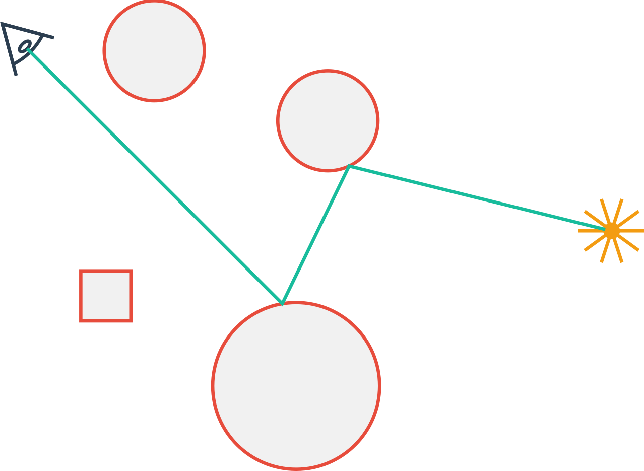
\includegraphics[width=3in, keepaspectratio]{../img/fractal/raytrace.pdf}
   \caption{Ray tracing}
   \label{fig:raytrace}
  \end{minipage}
  \begin{minipage}{0.5\hsize}
   \center
   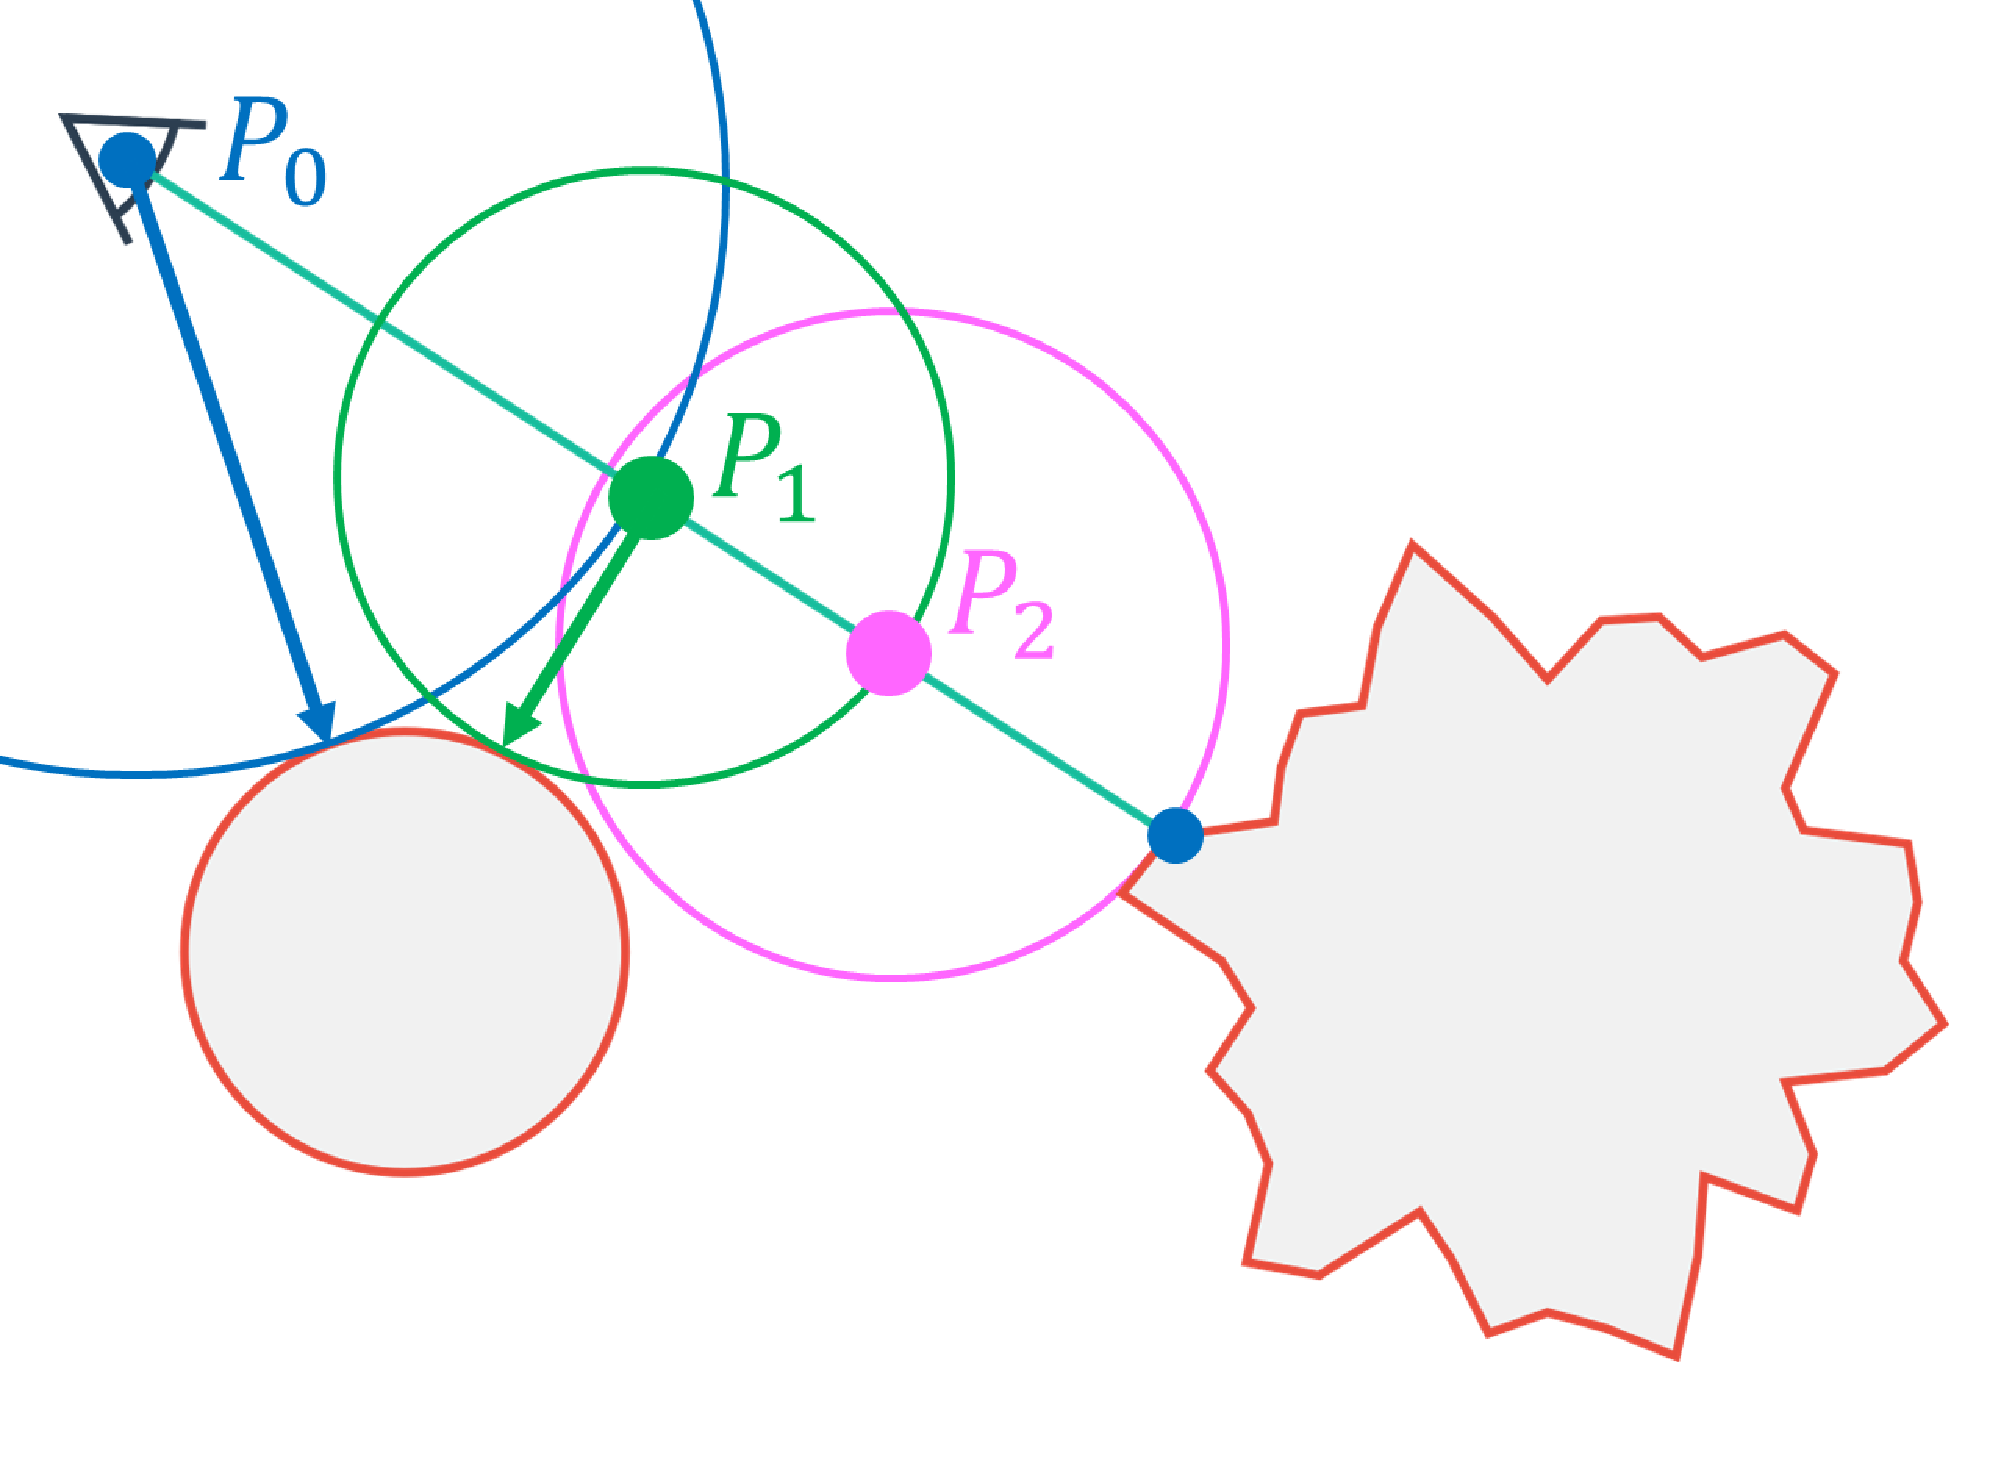
\includegraphics[width=3in, keepaspectratio]{../img/fractal/raymarching.pdf}
   \caption{Ray marching}
   \label{fig:raymarch}
  \end{minipage}
 \end{figure}

\subsection{Escape-time Fractals}

\textit{Escape-time Fractals}は複素平面上の点に対して,特定の漸化式を計算し,
その点の軌道の収束,発散を見ることで描画されるフラクタルである.
Escape-time Fractalsで代表的なものが\emph{マンデルブロ集
合}(\textit{Mandelbrot set})である.
複素平面上の点$c$に対して,以下に示す漸化式を計算し,$\displaystyle \lim_{n
\to \infty} z_n$が無限大に発散しないものをマンデルブロ集合とよぶ.
\begin{align*}
 z,~c \in \mathbb{C} \quad
 \begin{cases}
  z_{n+1} = z^2_{n} + c \\ z_0 = 0
 \end{cases}
\end{align*}

図\ref{fig:mandelbrot}において,赤で縁取られた黒い部分がマンデルブロ集合
である.その他の部分については,発散と判定されるまでの計算の回数によって
色をつけた.
マンデルブロ集合はその単純な式から,描画する位置や拡大率によって驚くほど
豊富なバリエーションの形を見ることができる.

各点における漸化式の計算はお互いに干渉しないので,そのままシェーダでの実
装が可能であるが,先に述べたDistance Estimationを用いることで,エイリア
シングノイズ等を避けてより精細に描画することができる.
これには\textit{Green Function}とよばれるマンデルブロ集合の陰関数を用いる.
導出はiqによる記事\footnote{distance rendering for fractals:
~\url{http://iquilezles.org/www/articles/distancefractals/distancefractals.htm}}
が詳しい.
Green Functionについてはマンデルブロ集合に関する詳細な議論となってしま
うので\cite{douady1984exploring}を参考にされたい.

その他のEscape-time fractalには図\ref{fig:julia}に示した
\emph{ジュリア集合}(\textit{Julia set})や\emph{ファトゥー集
合}(\textit{Fatou set})等がある.

\begin{figure}[htbp]
 \begin{minipage}{0.49\hsize}
  \center
   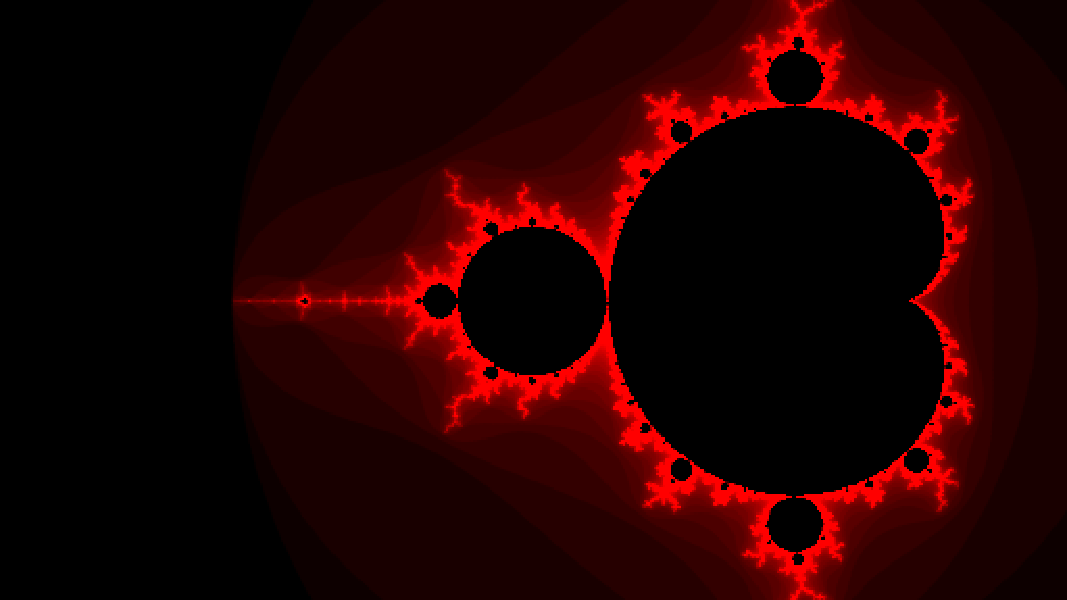
\includegraphics[width=3in, height=3in, keepaspectratio]{../img/fractal/mandelbrot.pdf}
   \caption{Mandelbrot set}
   \label{fig:mandelbrot}
 \end{minipage}
 \begin{minipage}{0.49\hsize}
  \center
  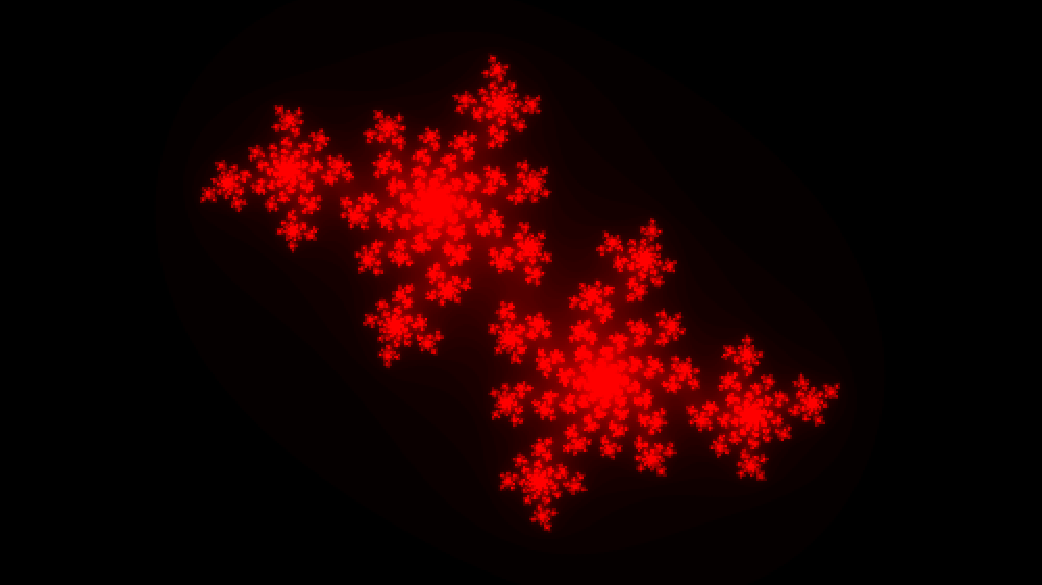
\includegraphics[width=3in, height=3in, keepaspectratio]{../img/fractal/julia.pdf}
  \caption{Julia set}
  \label{fig:julia}
 \end{minipage}
\end{figure}

\subsection{Distance Estimated 3D Fractals}

マンデルブロ集合は数あるフラクタルの中でも特に複雑な形状を見せるものであった
ので,その三次元への拡張も古くから興味が持たれてきた.
例えば,ジュリア集合を四元数を用いて計算した
\textit{Quaternion Julia 3D fractal}~\cite{hart1989ray}が1989年に発表され
ている.
しかし,この形状は図\ref{fig:qjulia}のように四元数による回転対称性をもつ
ため,形状が単純でフラクタルコミュニティの満足のいくものではなかった.

その他にもマンデルブロ集合のような複雑な三次元フラクタルを描画しよう試み
が様々にあった.
それらについてはDaniel White (twinbee)がまとめている
\footnote{Skytopia -The Mystery of the REAL, 3D Mandelbrot Fractal:~
\url{http://www.skytopia.com/project/fractal/mandelbrot.html}}.

そのような中で,2003年に発表された阿原・荒木による四次元クライン群の一種
である\textit{Quasi Fuchsian 3D Fractals}~\cite{ahara2003sphairahedral}
は,ある程度の複雑性を持った三次元形状をもつフラクタルで
あった.そのため,コミュニティに大きな影響を与えたと言われている.
その形状のひとつを図\ref{fig:quasi-fuchsian-3d}に示した.
このフラクタルに関しては2章で触れる.

\begin{figure}[htbp]
  \begin{minipage}[t]{0.49\hsize}
   \center
   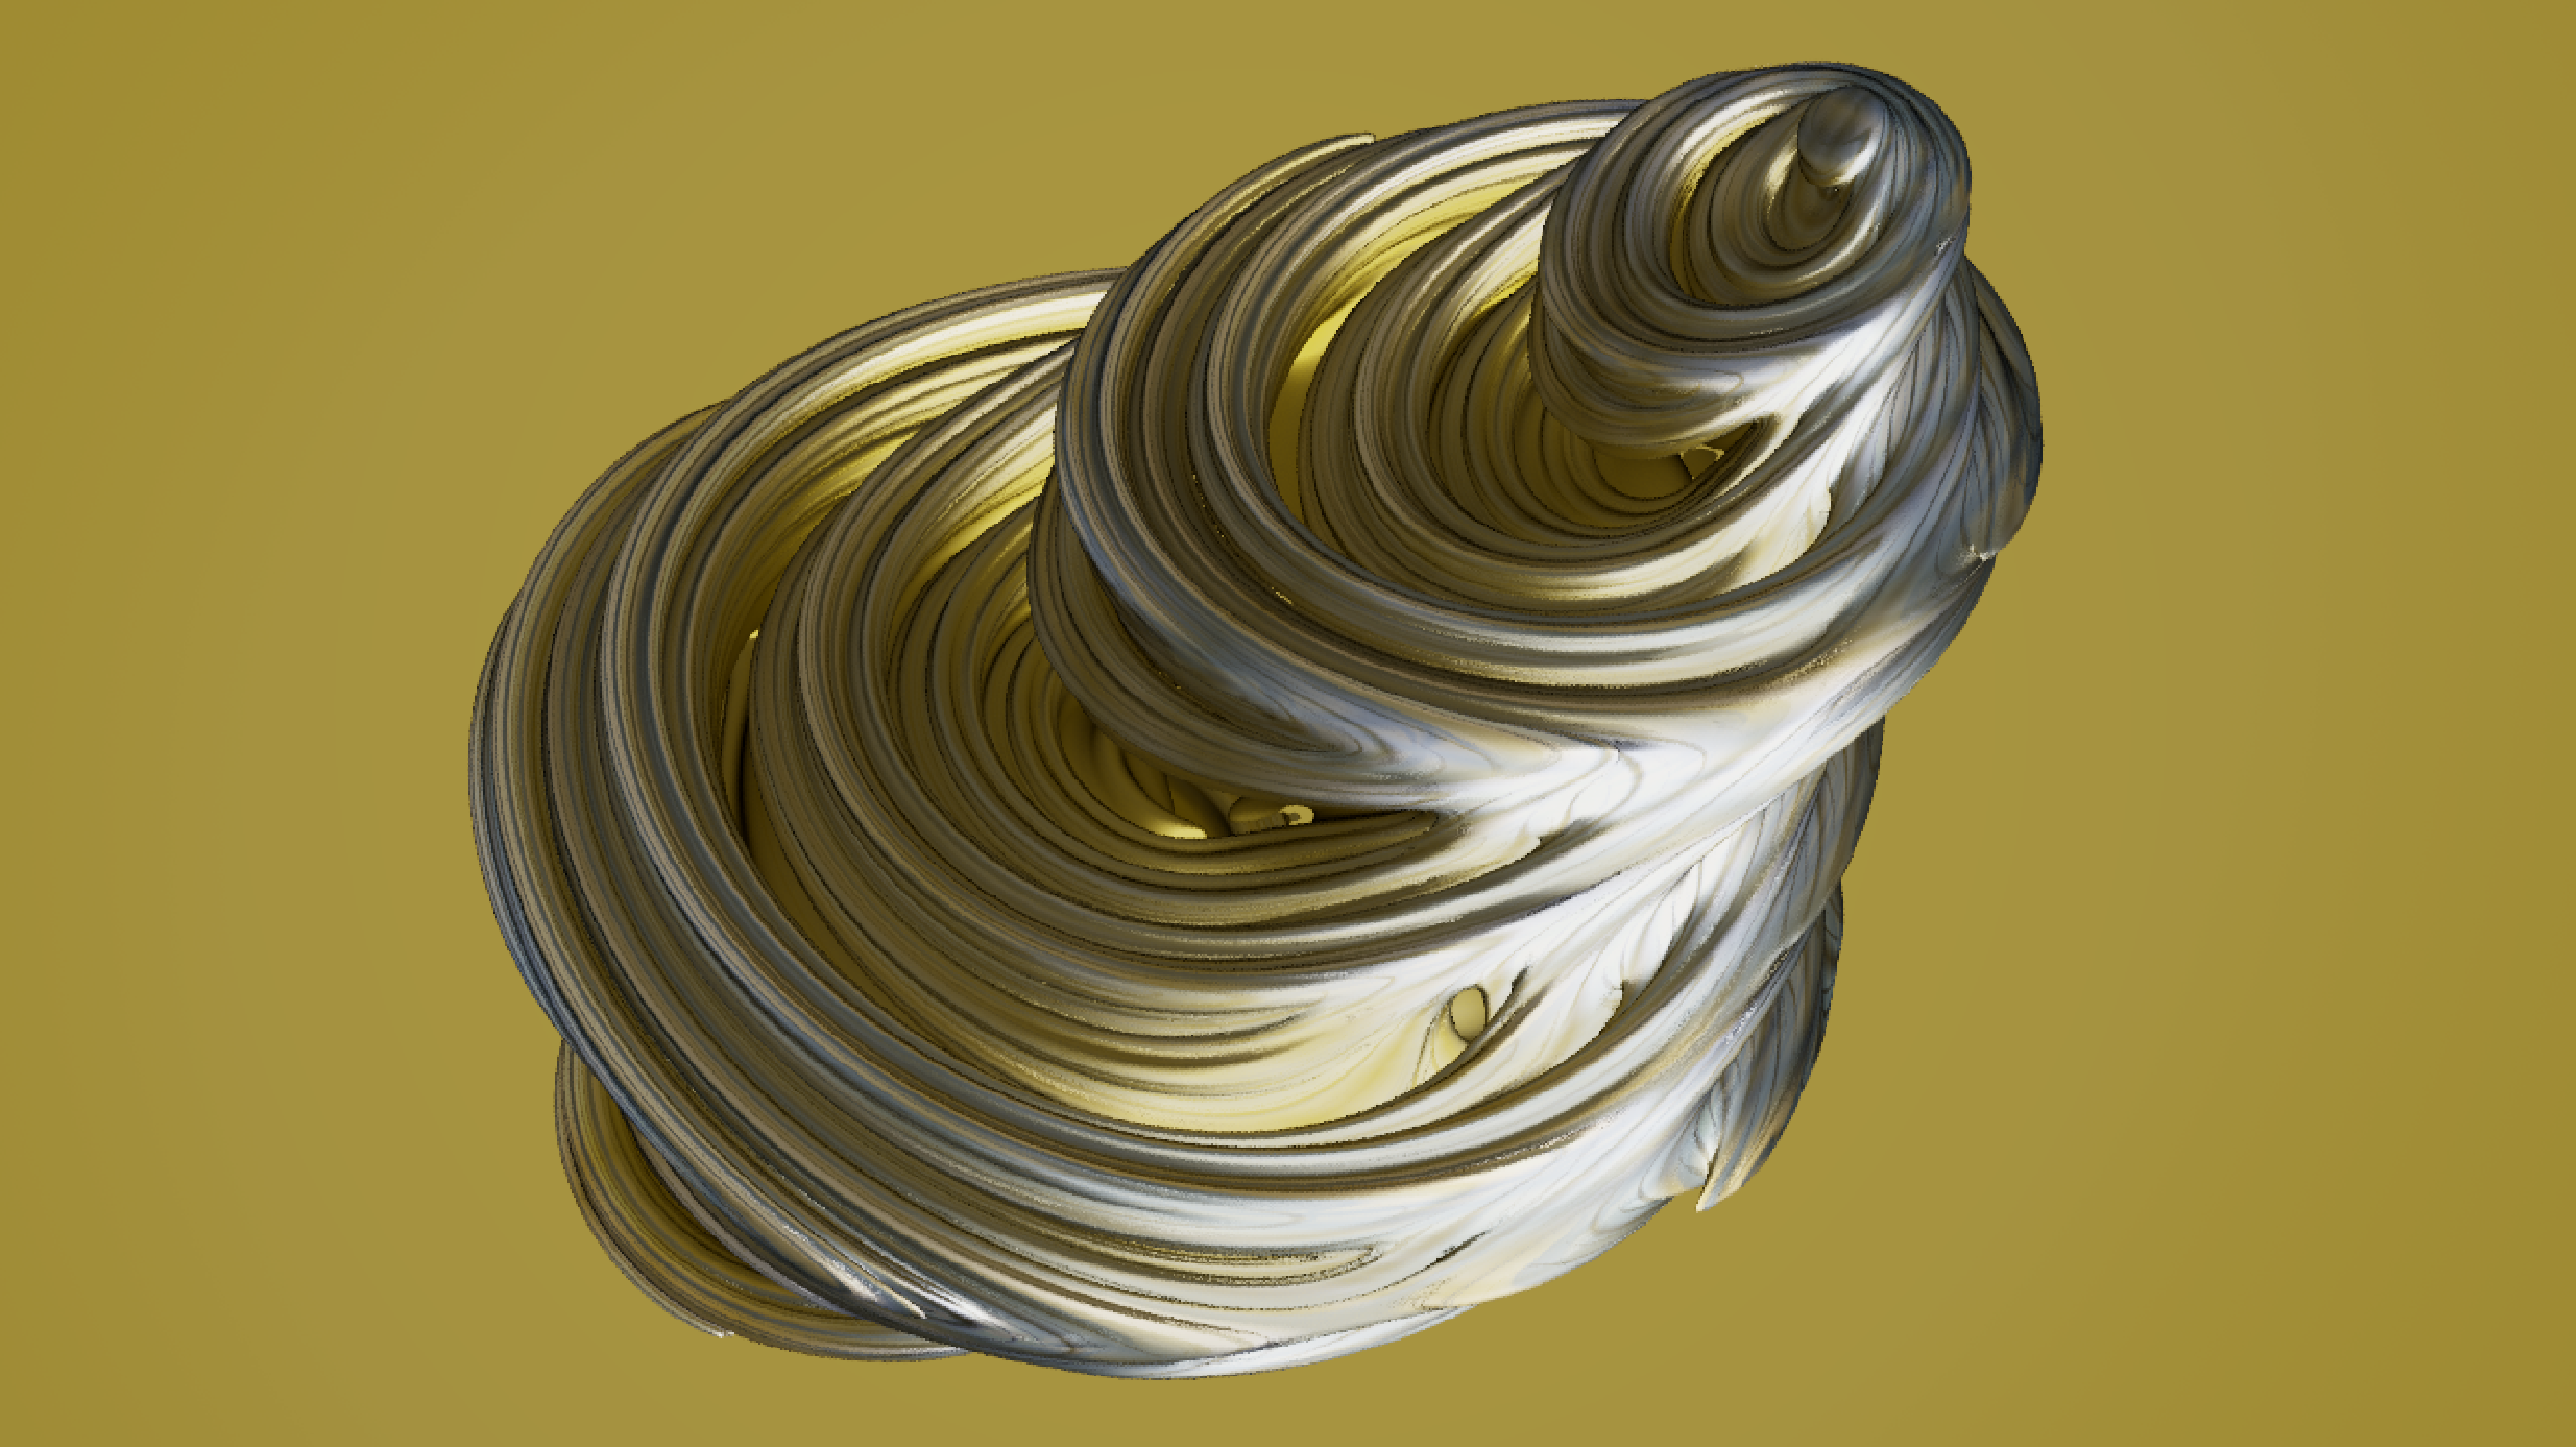
\includegraphics[width=3in, height=3in, keepaspectratio]{../img/fractal/qjulia.pdf}
   \caption{Quaternion Julia rendered with Fragmentarium}
   \label{fig:qjulia}
  \end{minipage}
 \begin{minipage}[t]{0.49\hsize}
  \center
  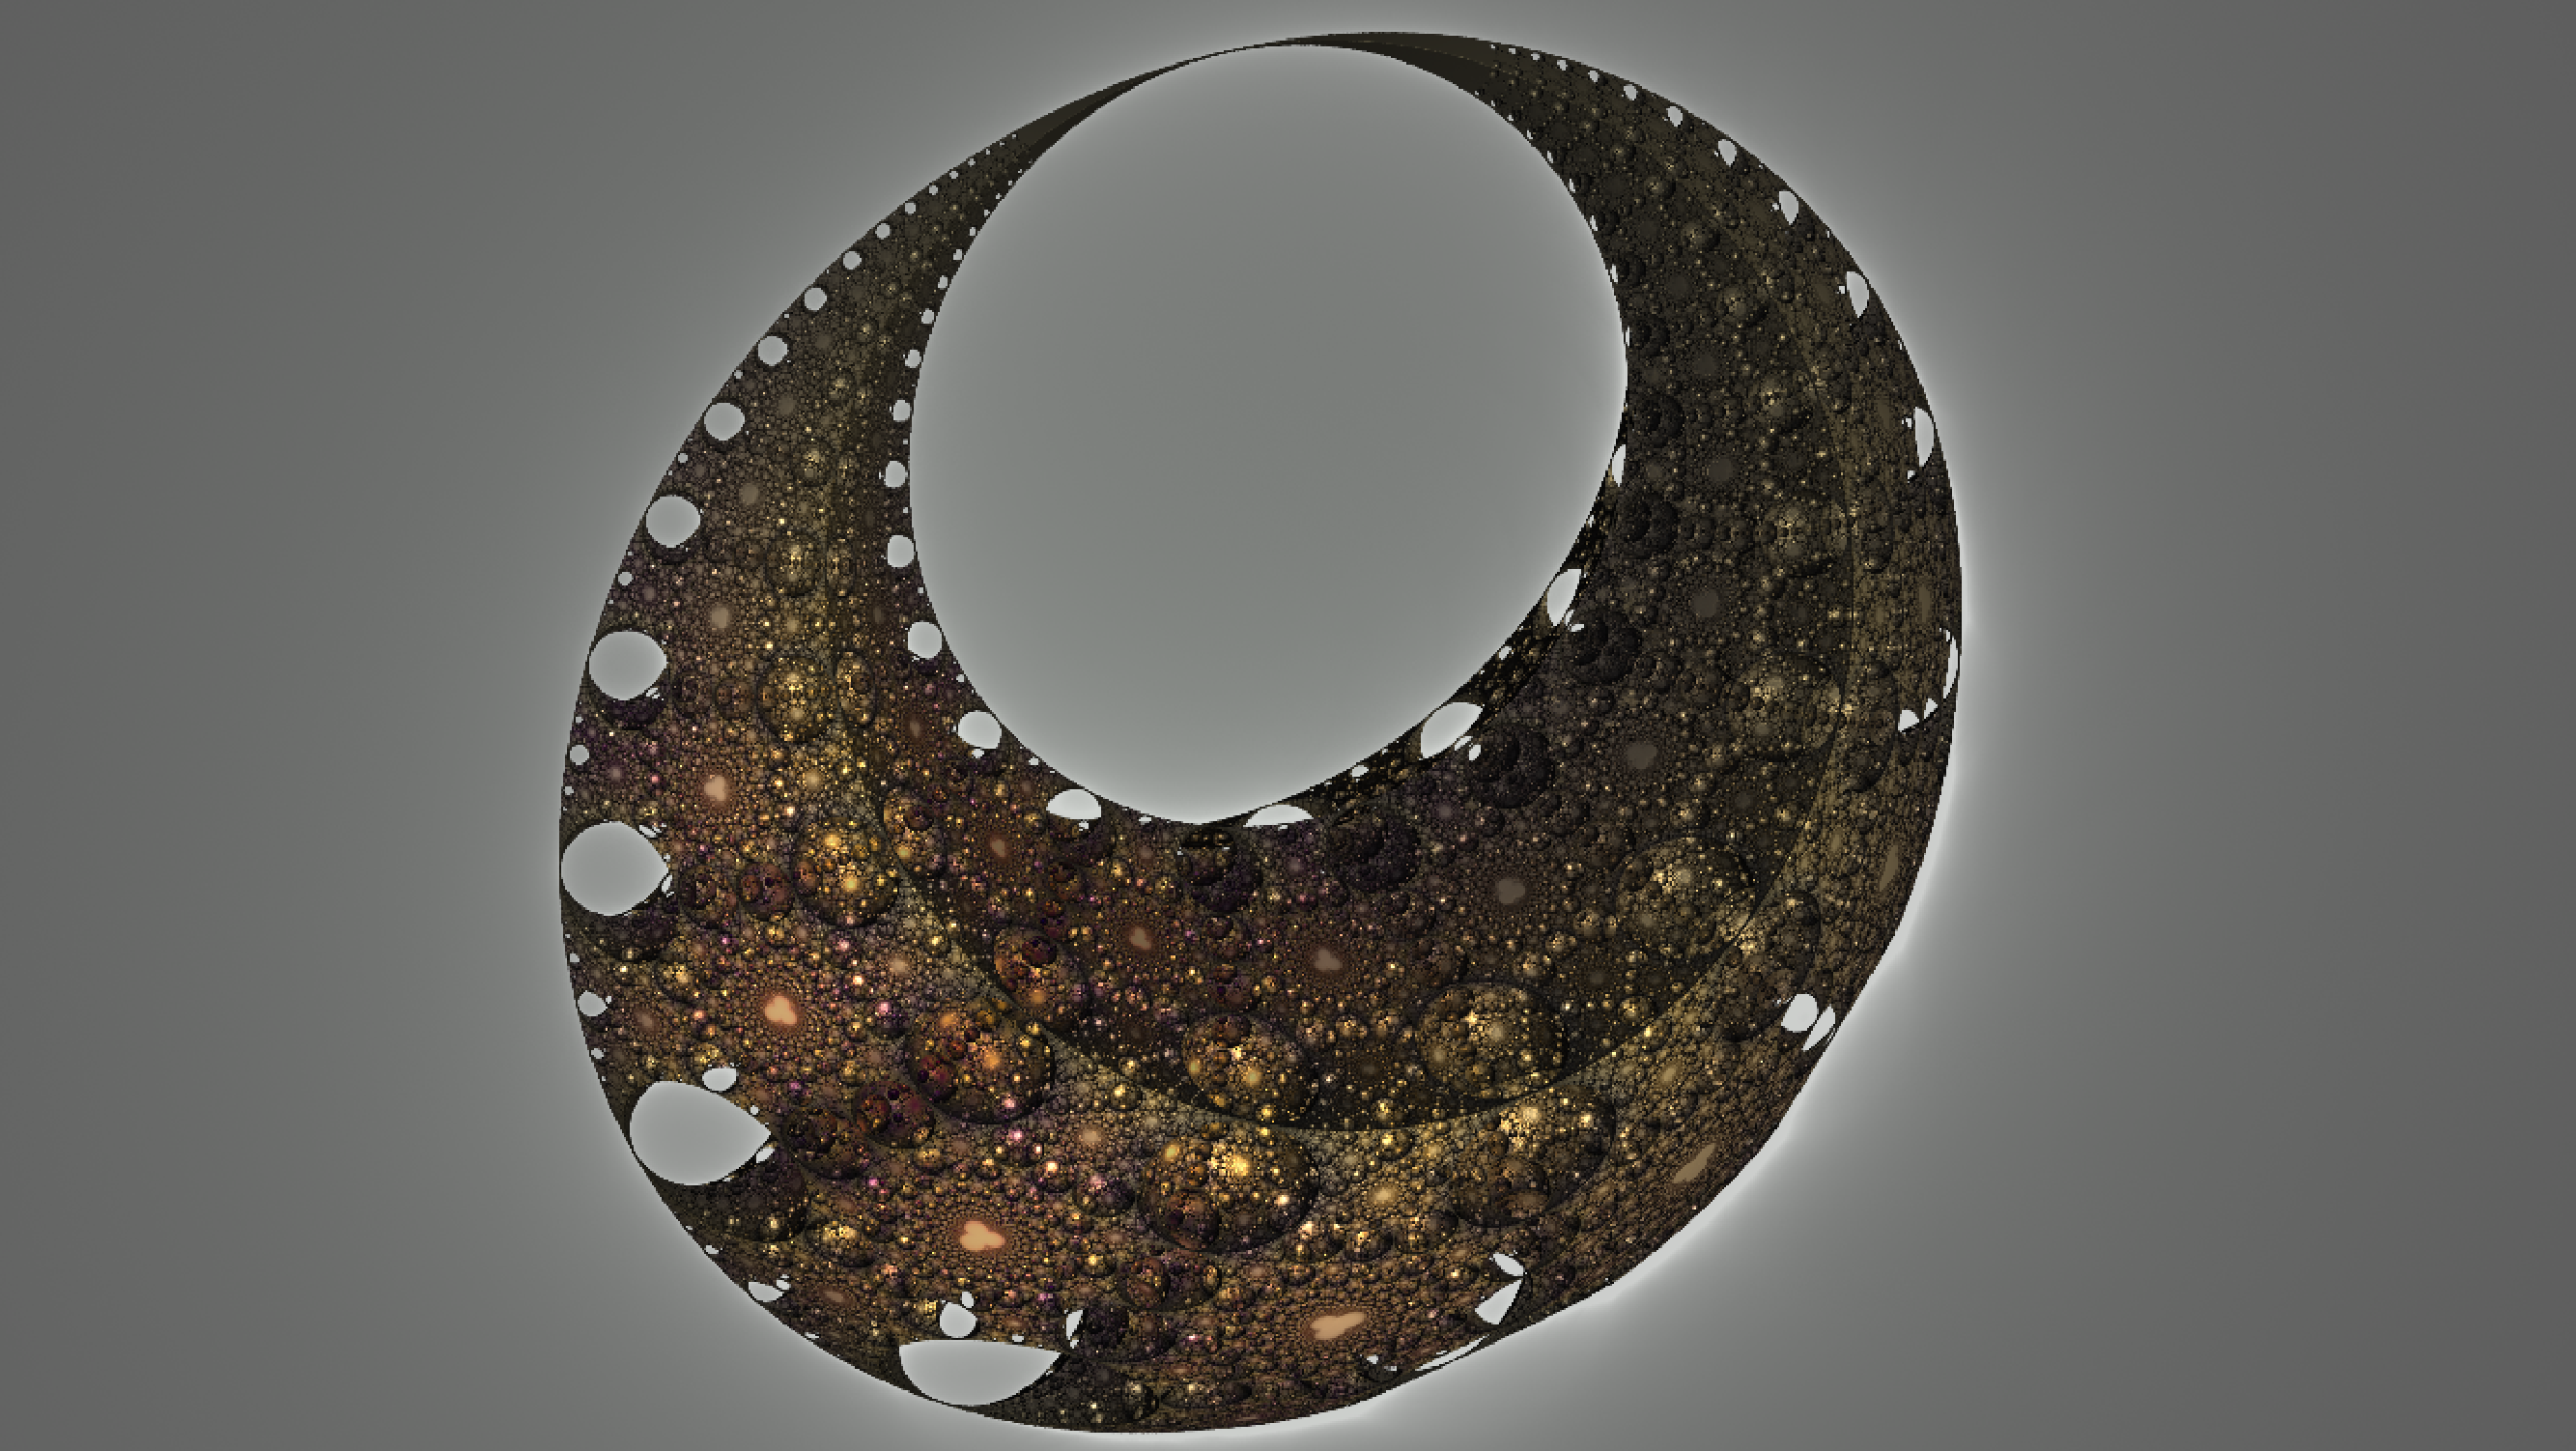
\includegraphics[width=3in, height=3in, keepaspectratio]{../img/fractal/quasi-fuchsian.pdf}
  \caption{Quasi Fuchsian 3D Fractal rendered with Fragmentarium
  (Knighty's script)}
  \label{fig:quasi-fuchsian-3d}
 \end{minipage}
\end{figure}

また,この時期から,コンピュータのグラフィクス性能が向上し,三次元のフラクタ
ル図形をリアルタイムに描画することができるようになった.
例えば,2004年にKeenan CraneはQuaternion JuliaをGPUによってリアルタイムに
描画している\footnote{Ray Tracing Quaternion Julia Sets on
the GPU:
~\url{https://www.cs.cmu.edu/~kmcrane/Projects/QuaternionJulia/}}.
iqは2007年にQuaternion Juliaをテーマにした4k intro~(実行ファイルのサイズ
を4kb以内に抑えたデモ作品),
\textit{kindernoiser}\footnote{kindernoiser:
~\url{http://www.pouet.net/prod.php?which=32549}}
を発表している.

その後,2009年に遂にマンデルブロ集合をうまく三次元に拡張した
\textit{Mandelbulb}が開発された.
これを皮切りに,次々と複雑な三次元フラクタルの式が開発された.
それらの多くはEscape-time fractalの一種であり,
Distance Estimationとレイマーチングを用いることで効率よくレンダリングす
ることができる.
これらのフラクタルの歴史と実装についてはMikael Hvidtfeldt Christensen
による一連の記事\footnote{Syntopia, Distance Estimated 3D Fractals:\\
\url{http://blog.hvidtfeldts.net/index.php/2011/06/distance-estimated-3d-fractals-part-i/}}
にまとめられている.
こちらも併せて参考にされたい.

これらのフラクタルをレンダリングするためのソフトウェアには\textit{Mandelbulb
3D}\footnote{Mandelbulb 3D:
~\url{http://mandelbulb.com/2014/mandelbulb-3d-mb3d-fractal-rendering-software/}}
や\textit{Mandelbulber}\footnote{Mandelbulber:
~\url{http://www.mandelbulber.com/}}が有名である.
シェーダベースのグラフィクスを開発するための環境である
\textit{Fragmentarium}\footnote{Fragmentarium:
~\url{http://syntopia.github.io/Fragmentarium/}}は
フラクタルのサンプルコードが豊富でアルゴリズムの学習に役立つ.
\textit{Fractal Lab}\footnote{Fractal Lab:
~\url{http://hirnsohle.de/test/fractalLab/}}はブラウザ上でGLSLを用いてフ
ラクタルをレンダリングすることができるウェブアプリケーションである.
この章で使われている図のいくつかはFractal LabとFragmentariumを用いてレン
ダリングした.

\subsubsection{Mandelbulb}

MandelbulbはDaniel WhiteとPaul Nylanderが2009年に開発した.
マンデルブロ集合の三次元拡張として広く知られている.

マンデルブロ集合の三次元の拡張において問題になるのは,三次元空間において
用いる代数である.
マンデルブロ集合の漸化式は複素数の乗算と加算で構成されている.
$z^2$は点$z$に原点中心の回転と拡縮を作用させ,加算$z + c$は平行移動を作用さ
せる.これによって点の軌道を考えることができる.
そのため,三次元空間の点において,軌道を考えることができるような$z^2$の
意味付けが必要であった.

Whiteは球面座標上においてマンデルブロ集合の漸化式を計算するアプローチを提案
した
\footnote{True 3D mandelbrot type fractal: \\
\url{http://www.fractalforums.com/3d-fractal-generation/true-3d-mandlebrot-type-fractal/}}
.
図\ref{fig:mandelbulb2}は$z_{n+1} = z_n^2 + c$を用いてレンダリングした結
果であるが,あまり複雑な形状は現れなかった.
しかし,その後Nylanderが式を高次の積を扱えるように拡張した.
図\ref{fig:mandelbulb8}は$z_{n+1} = z_n^8 + c $という式でレンダリングさ
れた形状であり,これがMandelbulbとして知られている.Whiteのウェブページ
\footnote{Skytopia:
~\url{http://www.skytopia.com/project/fractal/mandelbulb.html}}には開発の
詳しい経緯がまとめられている.

また,Mandelbulbも通常のマンデルブロ集合と同様にDistance Estimationによっ
て形状への最短距離を求めることができるため,レイマーチングで描画す
ることができる.

\begin{figure}[h!tbp]
 \begin{subfigure}{0.49\hsize}
  \center
  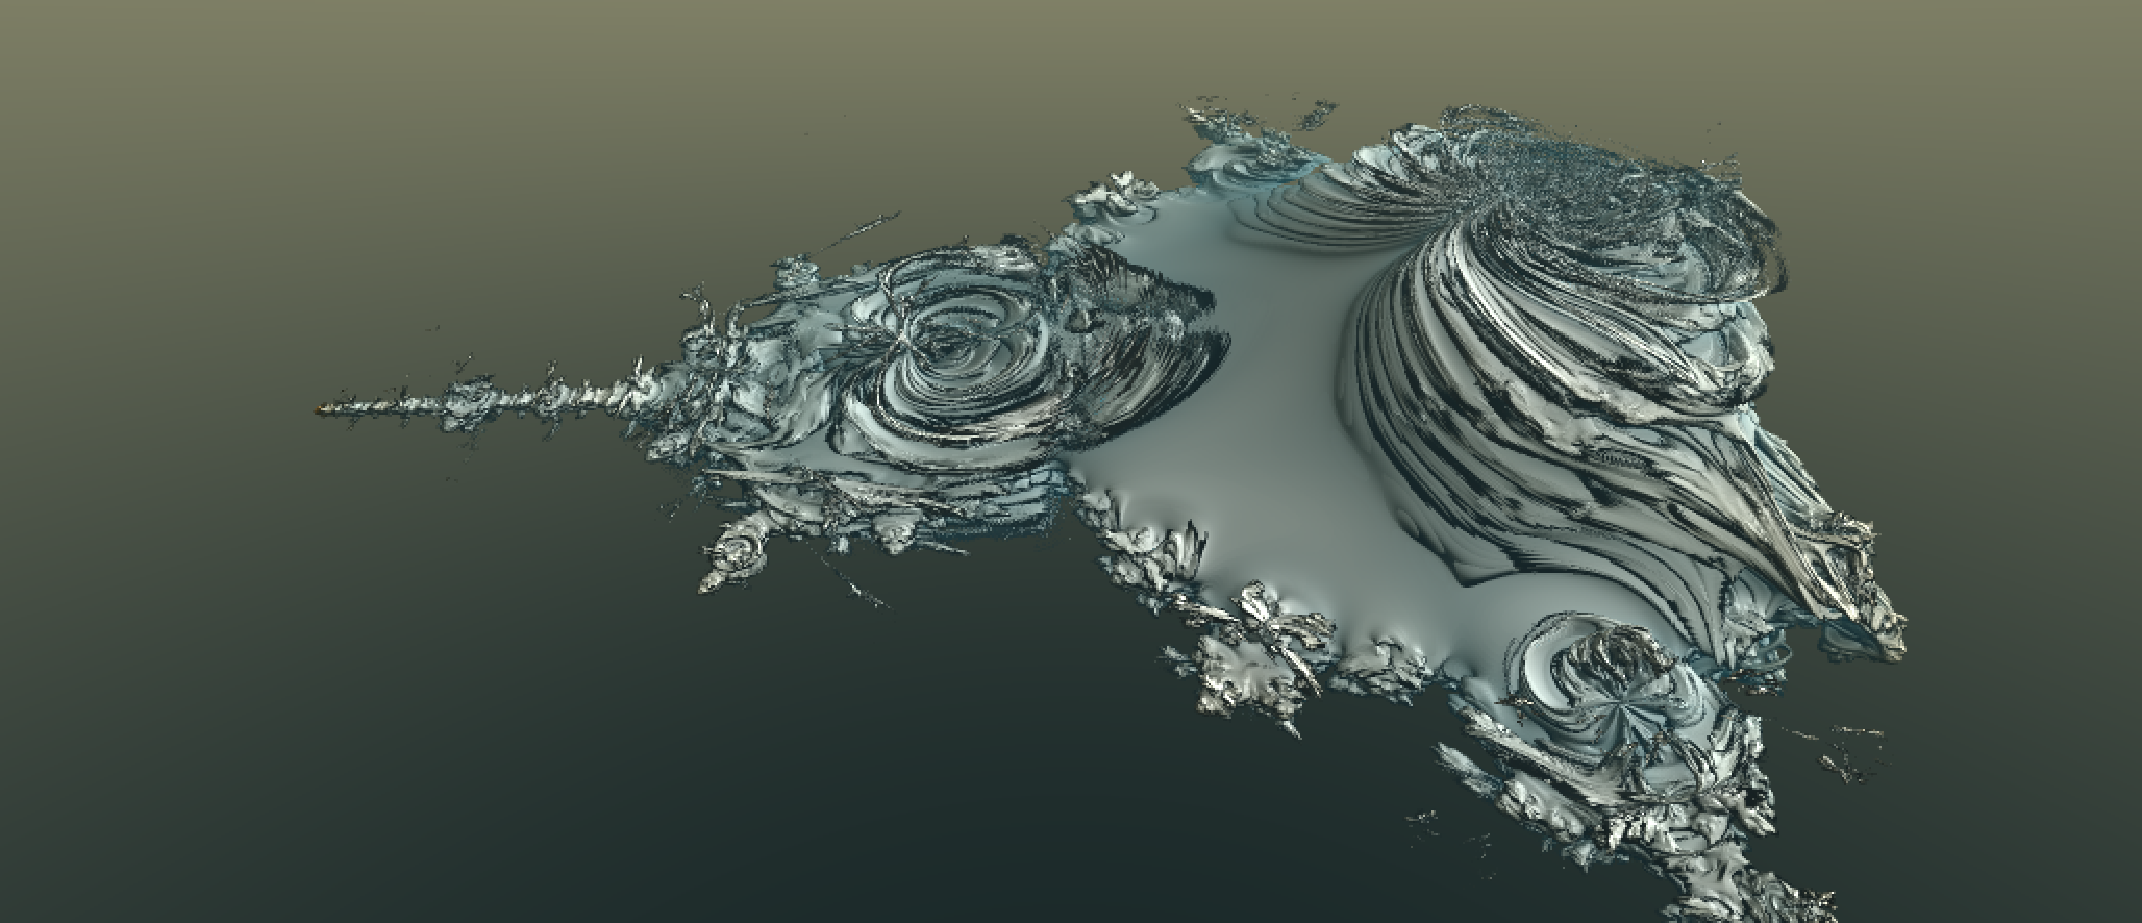
\includegraphics[width=3in, height=3in, keepaspectratio]{../img/fractal/mandelbulb2.pdf}
  \caption{$z_{n + 1} = z_n^2 + c$}
  \label{fig:mandelbulb2}
 \end{subfigure}
 \hspace*{\fill}
 \begin{subfigure}{0.49\hsize}
  \center
  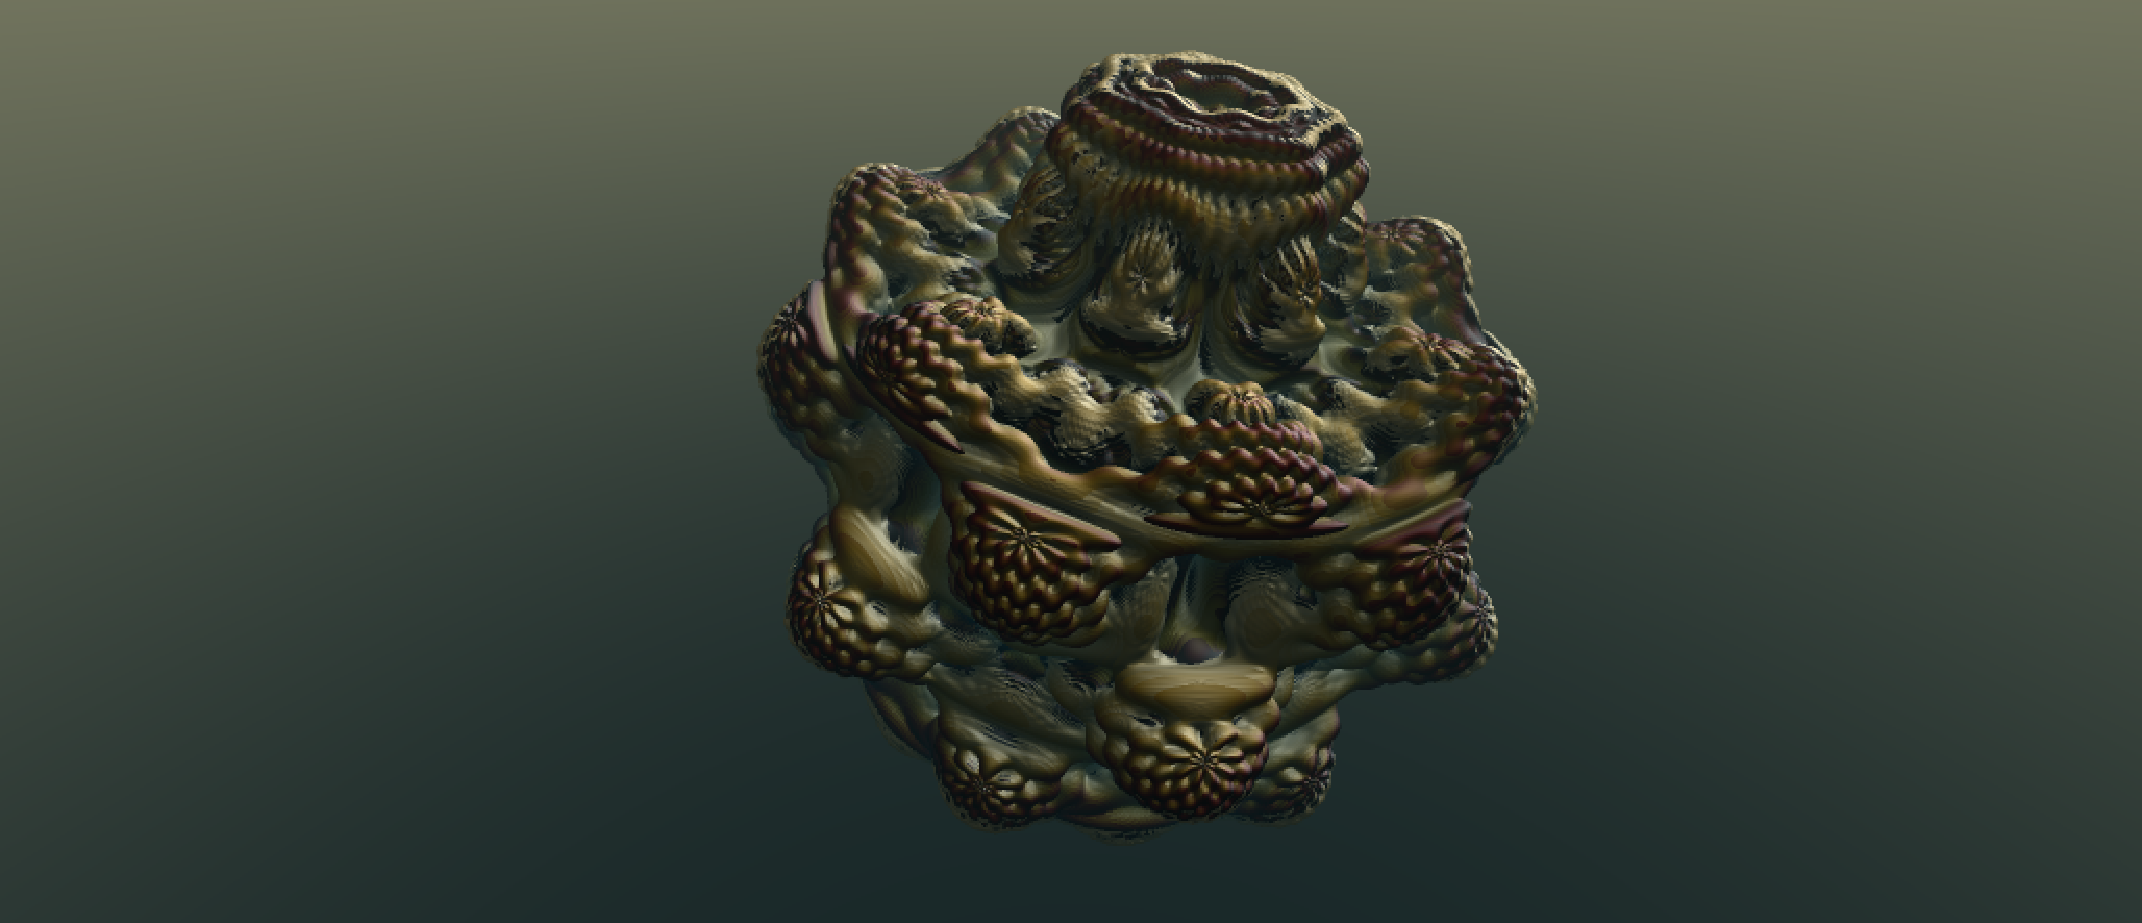
\includegraphics[width=3in, height=3in, keepaspectratio]{../img/fractal/mandelbulb8.pdf}
  \caption{$z_{n+1} = z_n^8 + c$}
  \label{fig:mandelbulb8}
 \end{subfigure}
 \caption{Mandelbulb rendered with Fractal Lab}
\end{figure}

\subsubsection{Mandelbox}

その後,2010年にTom Loweによって\textit{Mandelbox}\footnote{Mandelbox:
~\url{https://sites.google.com/site/mandelbox/what-is-a-mandelbox}}が開発
された.
Mandelboxも三次元空間におけるEscape-time fractalである.
漸化式は次のようになる.
\begin{align*}
 z_{n+1} = scale * spherefold(minR,~boxfold(z_n)) + c
\end{align*}
ここで\textit{boxfold}は$x=\pm1,~y=\pm1,~z=\pm1$を頂点にもつ立方体の各面
に対して,点がその外側にある場合にそれらの面に関する反転を行なう操作である.
\textit{spherefold}は点が原点中心の球の内側にある時にその球に関す
る反転を行う操作である.
ただし,球の反転は中心付近を無限遠点付近へと移してしまうため,漸化式の計算途中
に中心付近を通る点が発散と判定されてしまう.
そこでspherefoldでは中心付近の点の反転をあらかじめ決めておいた最小の半
径における反転で置きかえることで軌道が発散しないようにしている.
球の半径を$R$,最小の半径を$r$としたときに,$z$に対するspherefoldは以下
の式になる.
\begin{align*}
 spherefold(R,~r,~z) = \begin{cases}
                  z~\frac{R^2}{r^2} & 0 \le |z| < r \\
                  z~\frac{R^2}{|z|^2} & r \le |z| < R
                 \end{cases}
\end{align*}

MandelboxのDistance Estimationでは漸化式の微分としてヤコビアンの積を用いる.
式の各操作のたびにヤコビアンを累積していき,
最終的な点の原点からの距離をヤコビアンの積で割ることで距離を近似的に求
めることができる.

\begin{figure}[h!tbp]
 \begin{subfigure}{0.49\hsize}
  \center
  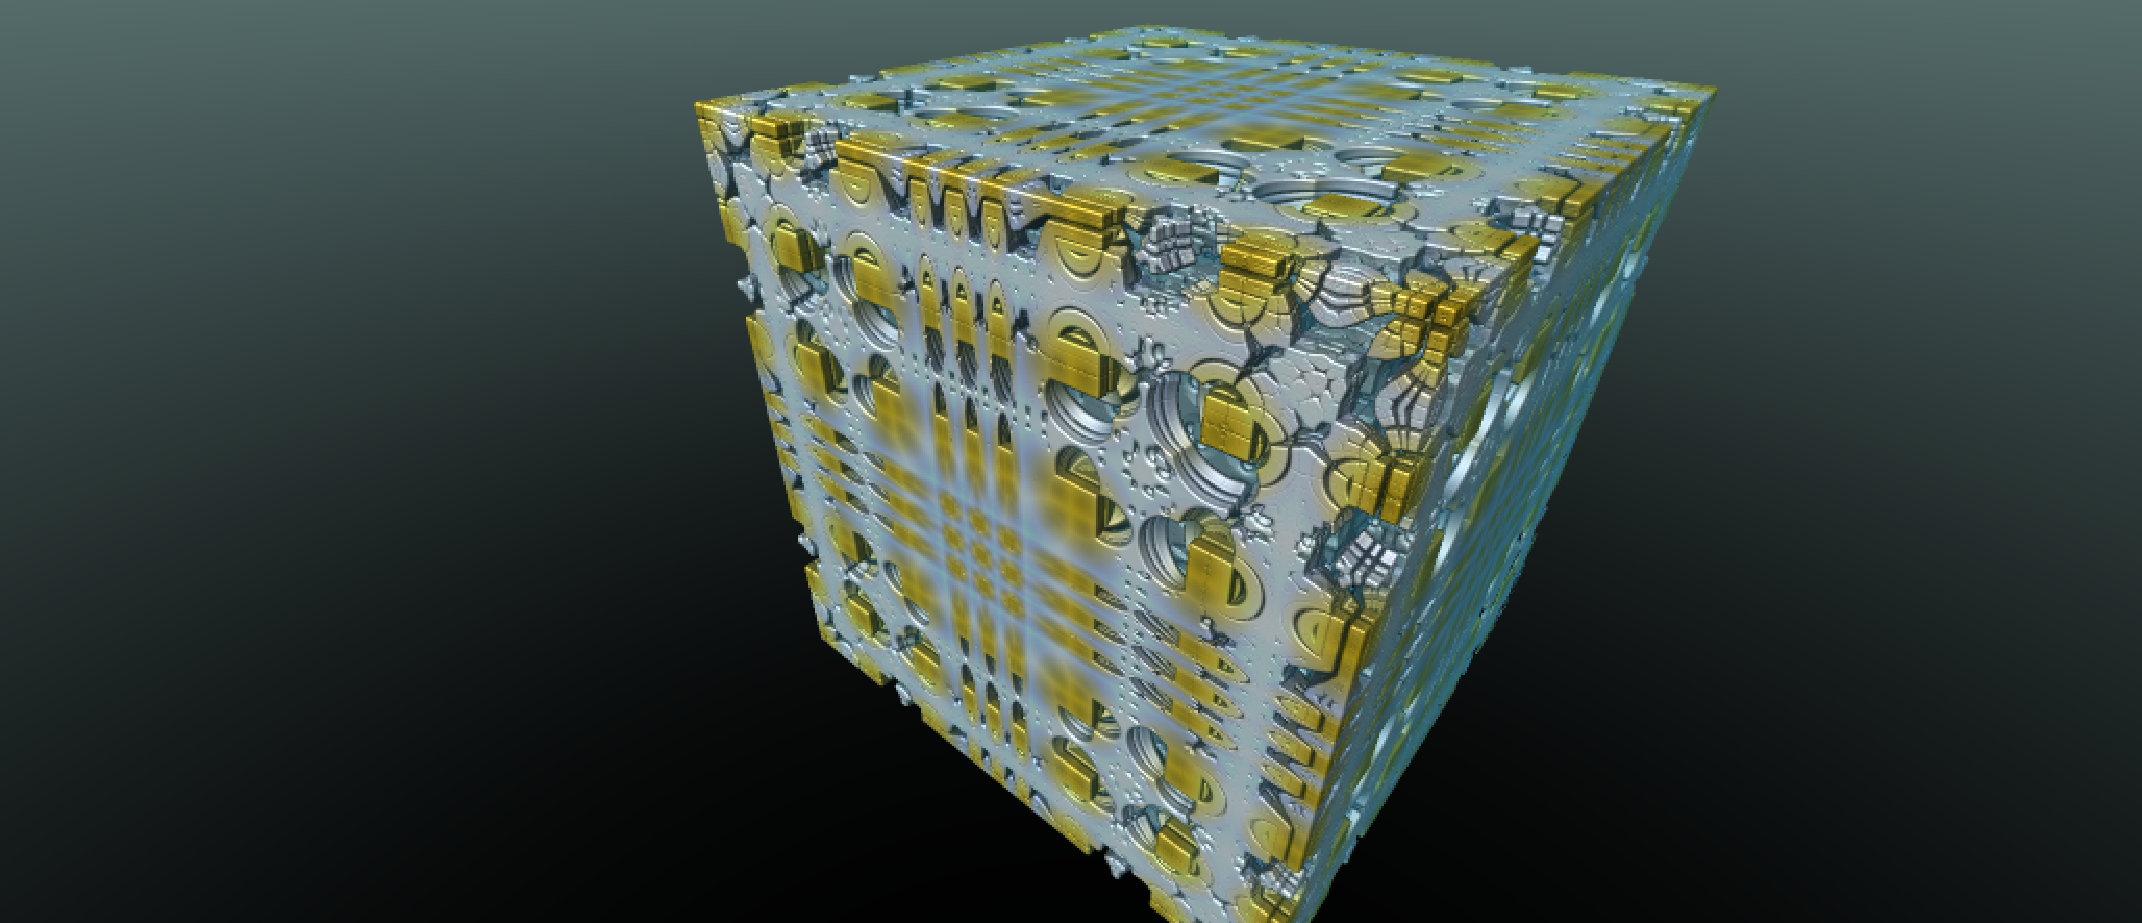
\includegraphics[width=3in, height=3in, keepaspectratio]{../img/fractal/mandelbox.pdf}
  \caption{}
  \label{fig:mandelbox1}
 \end{subfigure}
 \hspace*{\fill}
 \begin{subfigure}{0.49\hsize}
  \center
  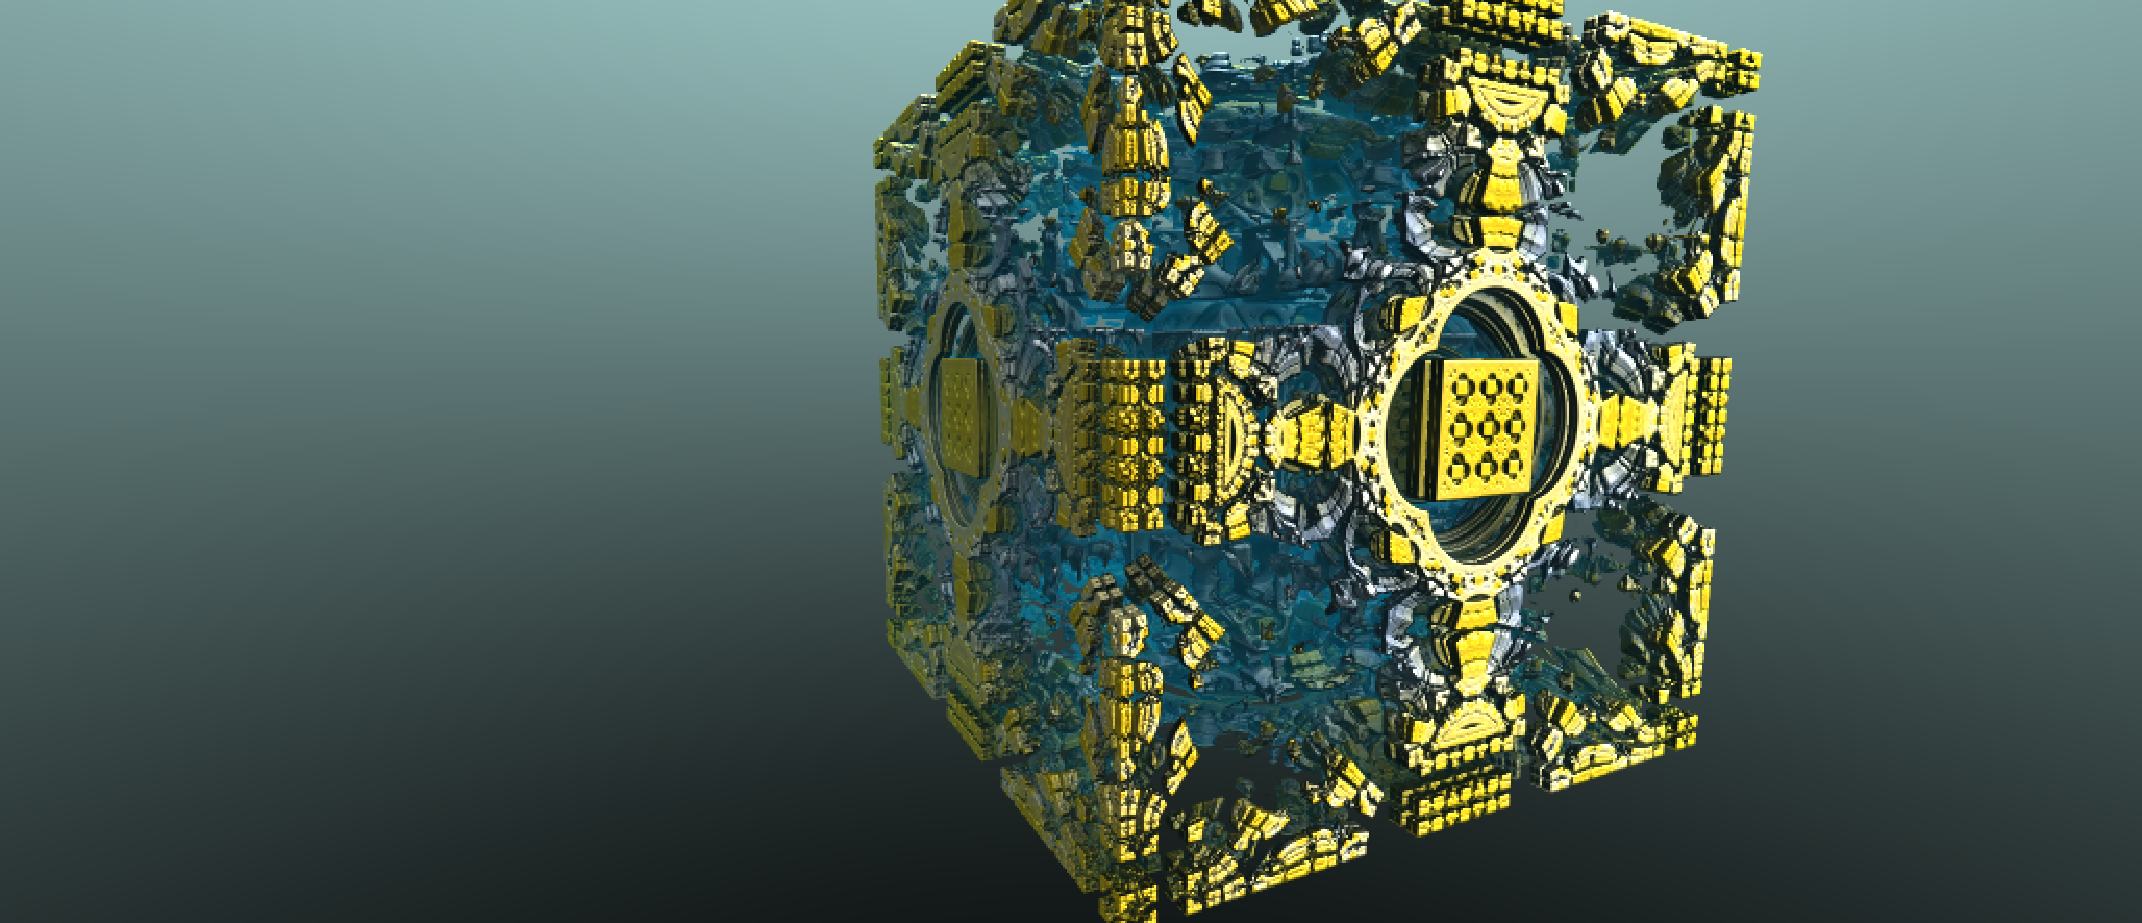
\includegraphics[width=3in, height=3in, keepaspectratio]{../img/fractal/mandelbox2.pdf}
  \caption{}
  \label{fig:mandelbox2}
 \end{subfigure}
 \caption{Mandelbox rendered with Fractal Lab}
 \label{fig:mandelbox}
\end{figure}


\subsubsection{Pseudo-Kleinian}

Mandelboxの登場以降は各$n$ごとに異なる式を組み合わせて漸化式を計算する
\textit{Hybrid System}によって,様々なフラクタル作品が作られている.

興味深いHybrid Systemの一つに\textit{pseudo-kleinian}がある.
これは球の反転に近い操作であるspherefoldと平行移動と同じような働きをする
boxfoldをうまく組み合わせることによって,可視化されたクライン群のような
形状が得られる式である.
これを図\ref{fig:pseudoKleinian}に示した.

\begin{figure}[htbp]
 \begin{minipage}{0.5\hsize}
  \center
  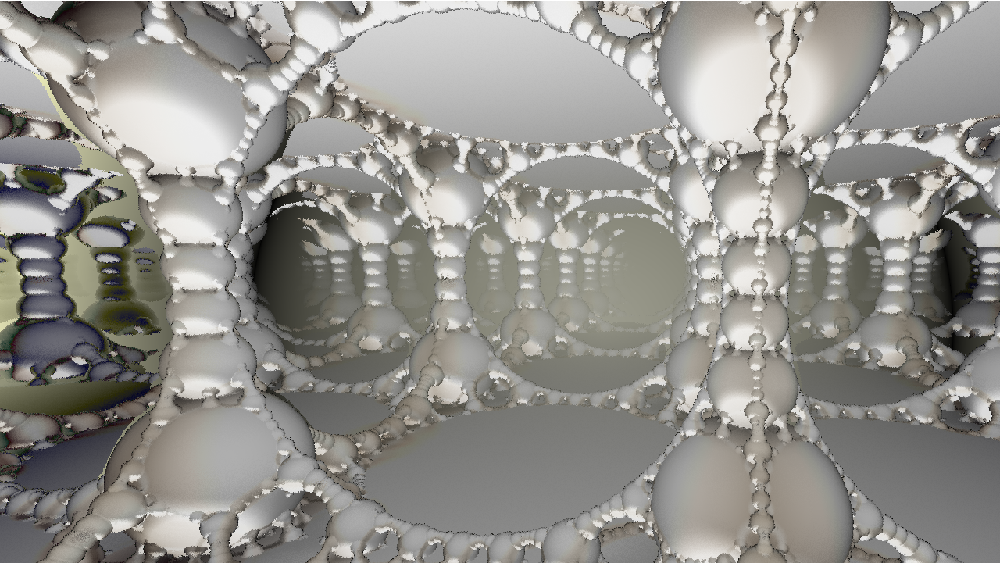
\includegraphics[width=3in, height=3in, keepaspectratio]{../img/fractal/pseudoKleinian.pdf}
  \subcaption{}
 \end{minipage}
 \begin{minipage}{0.5\hsize}
  \center
  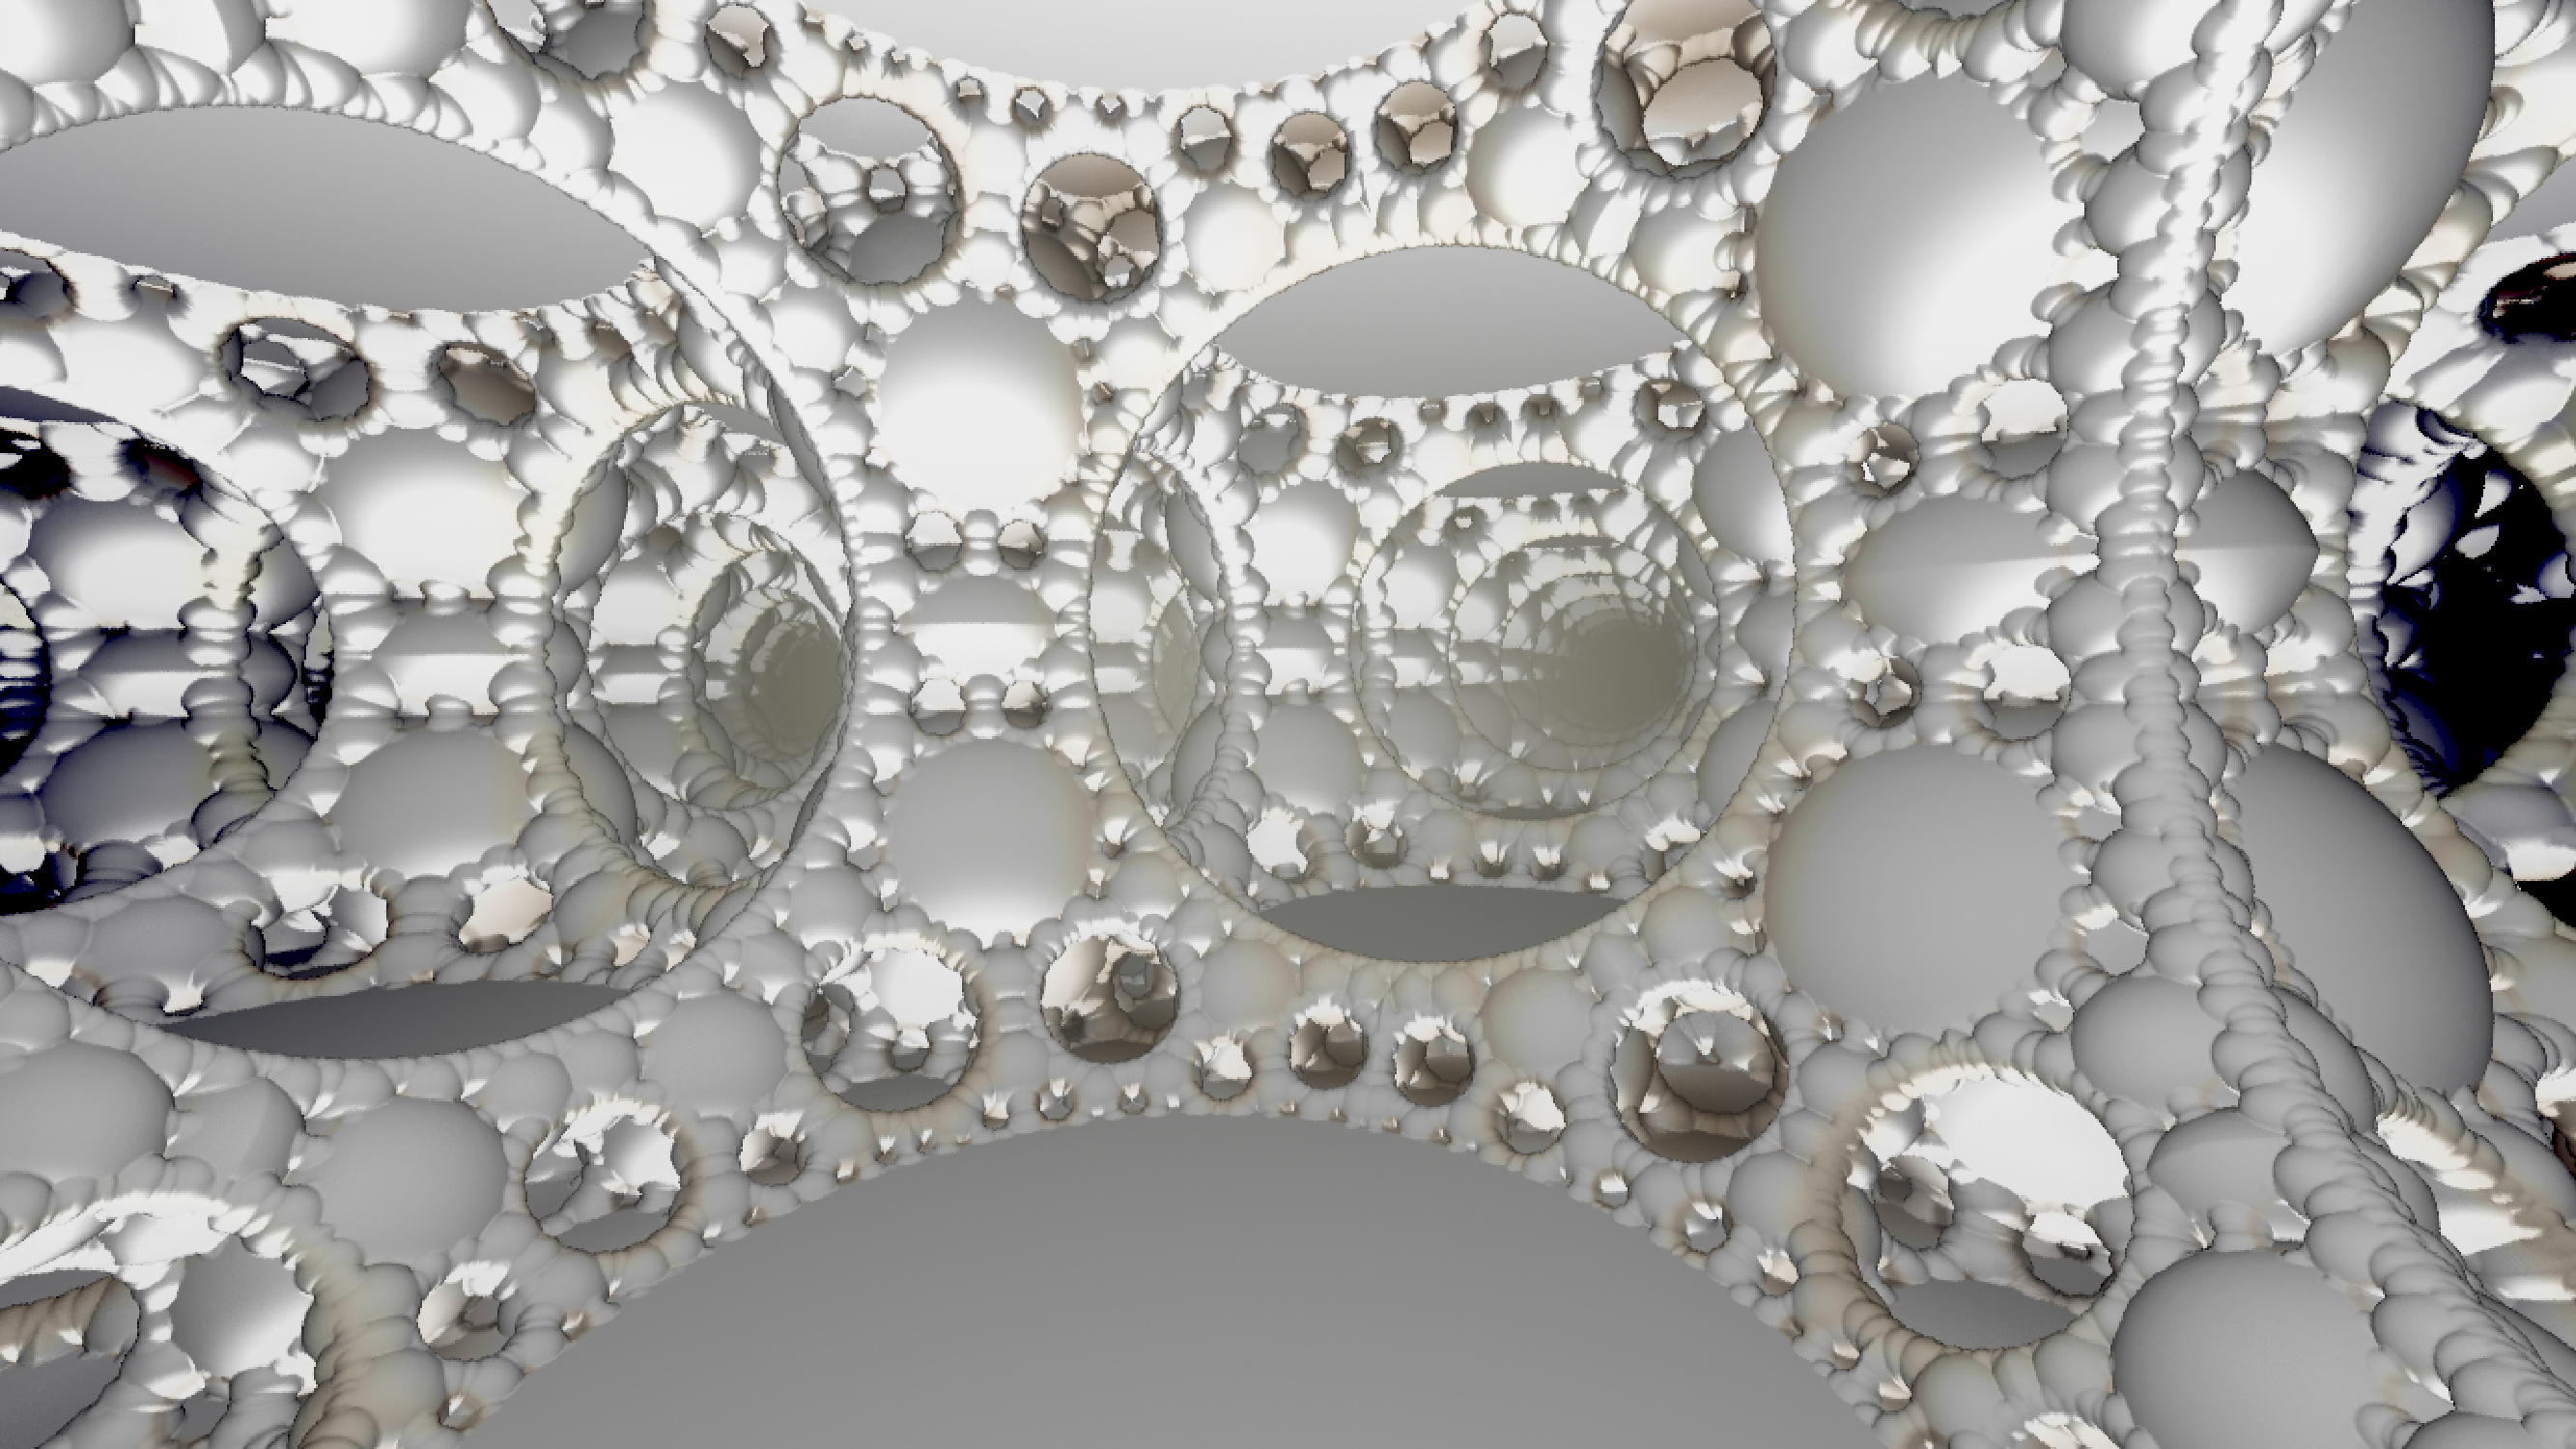
\includegraphics[width=3in, height=3in,
  keepaspectratio]{../img/fractal/pseudo-kleinian2.pdf}
  \subcaption{}
 \end{minipage}
  \caption{Pseudo-kleinian rendered with Fragmentarium}
  \label{fig:pseudoKleinian}
\end{figure}


\subsection{Coloring by Orbit Trap}

フラクタルのレンダリングにおいてカラーリングは重要な要素である.
Escape-timeアルゴリズムを用いたフラクタルのカラーリングには,主に\textit{
Orbit Trap}とよばれる手法が使われる.
図\ref{fig:mandelbox}のMandelboxもOrbit Trapを用いて色がつけられている.

Orbit trapはtrapとよばれる点や直線などの図形を空間上に置いておき,
trapと漸化式の計算で得られる軌道の点との位置関係から色を付ける方法である.
図\ref{fig:orbitTrap}はマンデルブロ集合とジュリア集合の漸化式において
$z_n$が桃色の領域に入った点を白く塗った.
これは桃色の領域に到達するまでの点の軌道を描いたと考えることができる.

また,この方法を応用すると画像をtrapに用いて,画像を変換で移した軌道を描
くことも可能である.
この手法は特に\textit{Bitmap Orbit Trap}ともよばれる.

\begin{figure}[htbp]
 \begin{minipage}{0.49\hsize}
  \center
  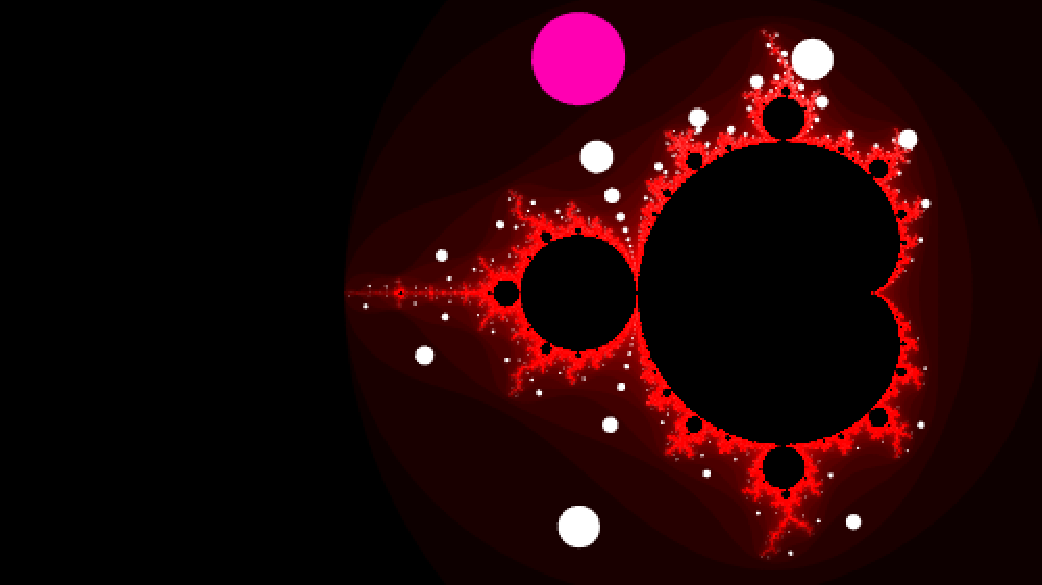
\includegraphics[width=3in, height=3in, keepaspectratio]{../img/fractal/mandelbrot-orbit.pdf}
  \subcaption{Mandelbrot set}
  \label{}
 \end{minipage}
 \begin{minipage}{0.49\hsize}
  \center
  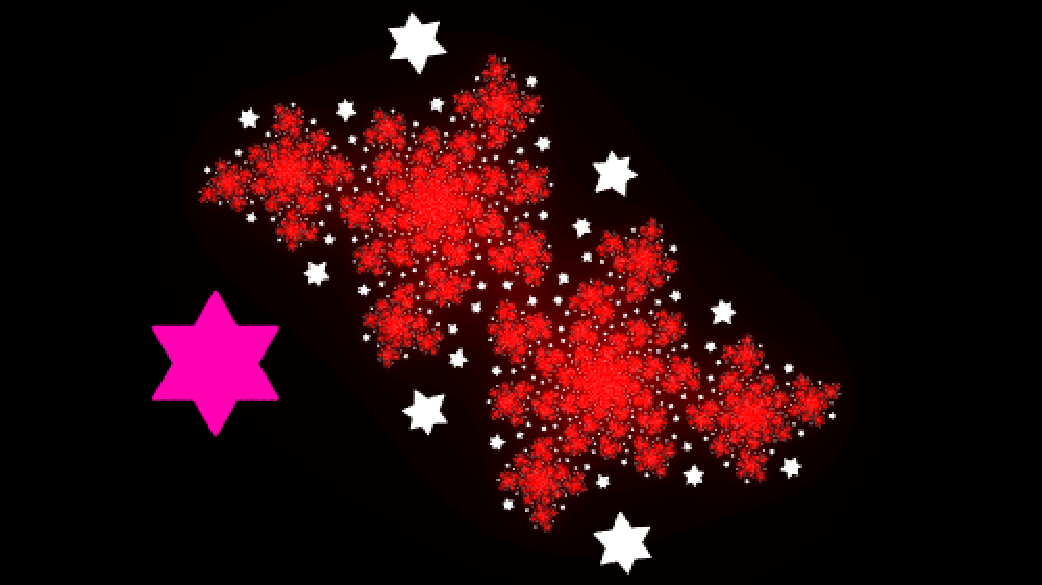
\includegraphics[width=3in, height=3in,
   keepaspectratio]{../img/fractal/juliaOrbit.pdf}
  \subcaption{Julia set}
  \label{}
 \end{minipage}
 \caption{Orbit trap}
 \label{fig:orbitTrap}
\end{figure}

\subsection{Iterated Function System}

もう一つ有名なアルゴリズムとして,\textit{Iterated Function System (IFS)}が
ある.IFSは点に複数の関数を反復的に作用させることでフラクタルを描画する
アルゴリズムの総称である.

IFSの描画アルゴリズムの一つとして,カオスゲームがある.
カオスゲームでは平面上の点をランダムにとり,その点にランダムに選んだ関数を作用させることを
繰り返すことで得られた点を描画する.
図\ref{fig:fern}はカオスゲームでレンダリングされたシダ植物である.
シェルピンスキーのギャスケットを含むその他のフラクタルもこの方法でレン
ダリングできるものがある.

IFSを拡張したフラクタルアートの一種に\emph{フラクタルフレーム}\textit{(Fractal
Flame)}~\cite{draves2003fractal}がある.
フラクタルフレームではIFSに用いる関数にメビウス変換などの非線形変換を用
い,美しくレンダリングされるようにカラーリングにも工夫が加えられている.
図\ref{fig:pseudoKleinian}はフラクタルフレームレンダラの一つである,
Apophysis 7Xを用いてレンダリングされたフラクタルフレームである.

IFSに関する書籍として\textit{Fractals
Everywhere}~\cite{BarnsleyMathematics201207}がある.
また,並列計算による高速化に関する論文に
~\cite{2010_fractal_flames}や\cite{Green:2005:GIF:1187112.1187128}がある.

\begin{figure}[htbp]
  \begin{minipage}{0.49\hsize}
   \center
   
\includegraphics[width=3in, height=3in, keepaspectratio]{../img/fractal/fern.pdf}
   \caption{Fern}
   \label{fig:fern}
 \end{minipage}
 \begin{minipage}{0.49\hsize}
  \center
  
\includegraphics[width=3in, height=3in, keepaspectratio]{../img/fractal/fractalFlame.pdf}
  \caption{Fractal Flame}
  \label{fig:fractalFlame}
 \end{minipage}
\end{figure}

\clearpage


%#!platex main.tex

\section{Kleinian Groups}

クライン群について学習する際には書籍『インドラの真珠』\cite{indra}を読む
ことを勧める.
インドラの真珠は数学者以外にもクライン群の魅力を伝えるために書かれた.
中には研究者レベルの高度な内容も扱うが,高校レベルの数学と簡単なプロ
グラムを組む能力があれば,自分で図をレンダリングしながら読み進めることができる.
この章では,クライン群に関する用語を確認した後にレンダリング手法と『イン
ドラの真珠』では言及のないクライン群の話題を紹介する.

\subsection{Conjugation}

クライン群を考えるうえで, 我々は様々な変換を扱う.
変換に関する操作において重要となるのが, \emph{共役}(\textit{Conjugation})
である.
共役を用いることで, ある変換をその性質を変えずに異なる座標において作
用させることができ, 複雑な変換をよりわかりやすい座標における変換としてみ
ることができる.

例えば, 図に示された矩形の中心における回転行列を求めたいとする.
原点を中心とした回転行列はよく知られているため, これを$T$とおく.
矩形の中心までの平行移動を表わす変換を$S$とすると, 求めたい行列$\hat{T}$
は$\hat{T} = STS^{-1}$で求めることができる.
これは, 矩形を一度原点まで平行移動で移し, 原点中心の回転を作用させ, 元の
場所まで戻すという操作に等しい.
ここで, 変換$\hat{T}$を$T$の共役, $S$を共役変換と呼ぶ.
$\hat{T}$はこの操作を行なった後でも回転を表わす変換であることに変わりはなく,
$\hat{T}$は回転と共役であるという.

\subsection{Group}

クライン群の\emph{群}(\textit{Group})という語は変換群のことを指す.
ここでは変換の集まりだと考えるとわかりやすい.
例えば,ある変換$f(z)$と$g(z)$,そしてそれらの逆変換の4つの変換を考える
とき,これらの組み合わせを合成することで得られる変換の集合を群とよぶ.
また,ここで群を構成した4つの変換を\emph{生成元}(\textit{Generator})とよ
ぶ.
クライン群は\emph{メビウス変換}(M\"obius Transformations)を生成元にもつ
群のなかで離散性という性質を持つものをいう.

ここでは,それぞれの変換を小文字のアルファベットで表し,その逆変換を大文字で綴る.
$f(z)$を$a$,$g(z)$を$b$とおくと逆変換は$A$,$B$となる.
変換の合成はアルファベットを並べて書くことで表す.
例えば合成変換$f(f(g(f(p))))$は$aaba$という語で表される.
また,上付文字はその変換の無限列とする.
例えば,$\overline{a}$は,$aaaaa...$というような変換$a$の無限列となる.
この無限列に対応する合成変換はどの点に作用させてもその点を変換$a$の
\emph{固定点}に移す.
固定点とは,$f(z) = z$となるような,変換を使って動かすことのできない点である.
 \begin{align*}
  Generators =
   \begin{cases}
    a \colon f(z) \\
    A \colon f^{-1}(z) \\
    b \colon g(z) \\
    B \colon g^{-1}(z)
   \end{cases}
  \quad
  Group =
   \begin{cases}
    aab\\
    abbbaB \\
    ABBAbba \\
    baBBAbaaa \\
    ...
   \end{cases}
 \end{align*}

\subsection{M\"obius Transformations}

二次元のメビウス変換は複素平面上に, ひとつの無限遠点を付け加えた拡張複素
平面$\hat{\mathbb{C}}$上で定義される.
これはリーマン球面とも呼ばれ, 拡張複素平面全体を球面として扱うことができ
る.
メビウス変換は一次分数変換とも呼ばれ,以下のように表わされる.
\begin{align*}
 a, b, c, d\in \hat{\mathbb{C}} \quad f(z) = \frac{az + b}{cz + d}
\end{align*}
我々になじみの深い平行移動,拡縮や回転といった変換もメビウス変換に含まれ
る.メビウス変換は,等角性や円円対応といった性質をもつ.

また,以下のように係数を2×2の複素数行列として扱うことで,代数として操作することが
できる.
例えば合成変換を行列の積として表すことができる.
\begin{align*}
  m = \left(
 \begin{array}{ccc}
  a & b \\
  c & d
 \end{array}
 \right)
\end{align*}

メビウス変換はおおまかに\emph{放物型}(\textit{Parabolic}), \emph{斜航
型}(\textit{Loxodromic}), \emph{楕円型}(\textit{Elliptic})の三種類に分
類される.
斜航型変換と楕円型変換は2つ,放物型変換は1つの固定点をもつ.
斜航型変換は単純な回転を除いた複素数による拡縮と共役である.
また斜航型変換の中でも,正の実数による拡縮と共役の
変換を\emph{双曲型}(\textit{Hyperbolic})と呼ぶ場合もある.
放物型は平行移動と共役で, 楕円型変換は回転と共役である.

クライン群の描画において,メビウス変換の分類は重要である.
なぜならば,楕円型変換を含む群の多くはクライン群にはなりえない.
また,放物型変換は固定点への収束が遅いという特徴をもつ.
これは後述する極限集合の描画の際に考慮することとなる.

\subsection{Circle Inversion}

円は複素平面に作用するメビウス変換を考えるうえで重要な図形である.
先に述べたように,メビウス変換によって円は円に移される円円対応という性質
をもつ.
ここでは円に関する反転(\textit{Circle Inversion})という操作をみる.
これは円弧を鏡とみた鏡映であり,無限遠点は円の中心と入れ替えられる.
また,メビウス変換を構成する変換の最小単位ともいえる.

点aを中心とする半径rの円に関する反転を$I(z)$とすると式は以下のようになる.
\begin{align*}
I(z) =
 \begin{cases}
  \frac{r^2}{\overline{z - a}} + a \quad &for \quad z \in \mathbb{C} - \{a\} \\
  a \quad &for \quad z = \infty\\
  \infty \quad &for \quad z = a
 \end{cases}
\end{align*}
また,半径が無限大の円は直線とすることで,その円に関する反転は直線
に関する反転と考えることができる.

図\ref{fig:circleInversion}は黒い円に関する反転によって移される図形を可
視化したものである.
緑色の矩形を観察すると,変換の前後で大きく形を歪められているが, その角は直
角が保たれている.
直線は無限遠点が円の中心へと移るため, 反転円の中心を通る円となる.
また, 桃色の円は操作の前後で円が保たれている.

円に関する反転は複素平面の向き付けを逆にしてしまうため, メビウス変換では
ないが, 2つの反転を合成することで双曲型のメビウス変換となる.
偶数個の円の反転を組み合わせることで, その他の種類のメビウス変換を構成することが
できる.
また, 円を球に拡張することで球に関する反転を考えることができる.
これを用いて三次元空間に作用するメビウス変換を構成することもできる.

\begin{figure}[htbp]
 \begin{center}
      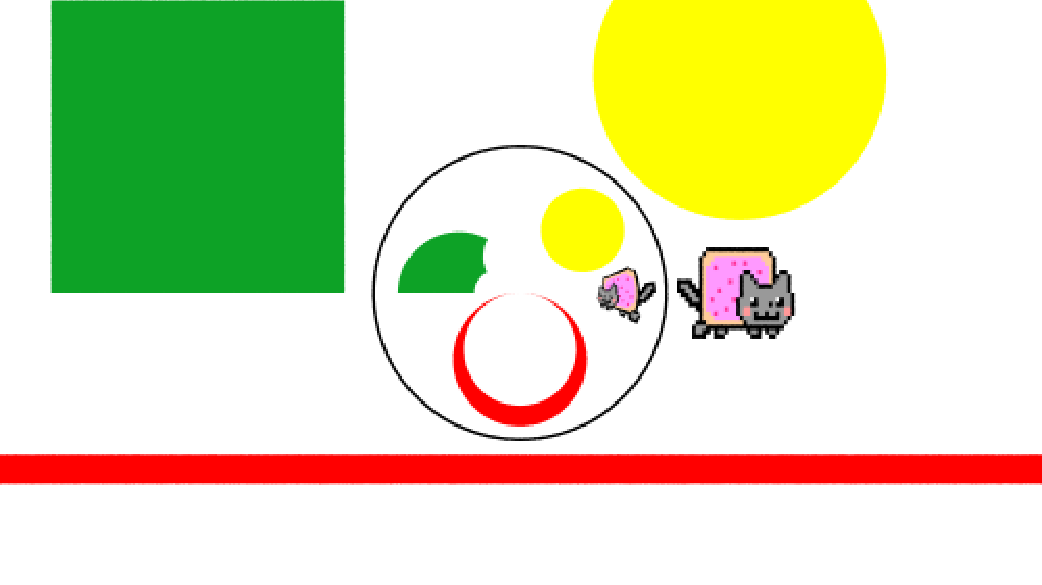
\includegraphics[width=3in, height=3in, keepaspectratio]{../img/klein/circleInversion.pdf}
    \caption{Circle Inversion}
    \label{fig:circleInversion}
 \end{center}
\end{figure}

\subsection{Stereographic Projection}

拡張複素平面はリーマン球面という名の通り, 球面で表すことで全
体をよく見ることができる.
複素平面を球面へと写像するためには, \emph{立体射影}({\it
stereographic projection})と呼ばれる方法がよく使われる.
地図の制作のため, 地球のような球面を平面に投影する方法が様々に考えられて
きたが, その中でも立体射影は角度と円を保つため, メビウス変換と相性が良い.

立体射影は簡単に説明すると以下のように行える.
ある球面上の点を$P$とおくと, $P$を立体射影で移した複素平面上の像は球面の北極
から$P$へと引いた直線と複素平面との交点となる.

図\ref{fig:stereoProject}は立体射影を図示したものである.
赤の円は単位円,青の直線はx軸を表している.
緑の直線において,北極以外の球面上の交点と,平面との交点が立体射影によっ
てお互いに移りあう点である.

Saul Schleimer, Henry Segermanはこれを利用した全天球画像へのエフェクトを
考案している\cite{spherical}.
図\ref{fig:spherical}は正距円筒図法(Equirectangular map)と球の内側からみ
た視点と, 複素平面とリーマン球面を可視化したものである.
このように, 複素平面上での回転は球の回転として表わすことができる.
\footnote{Spherical Droste video: \url{https://www.youtube.com/watch?v=qvh-EAipIUk\&t=4s}}

\begin{figure}[htbp]
 \center
 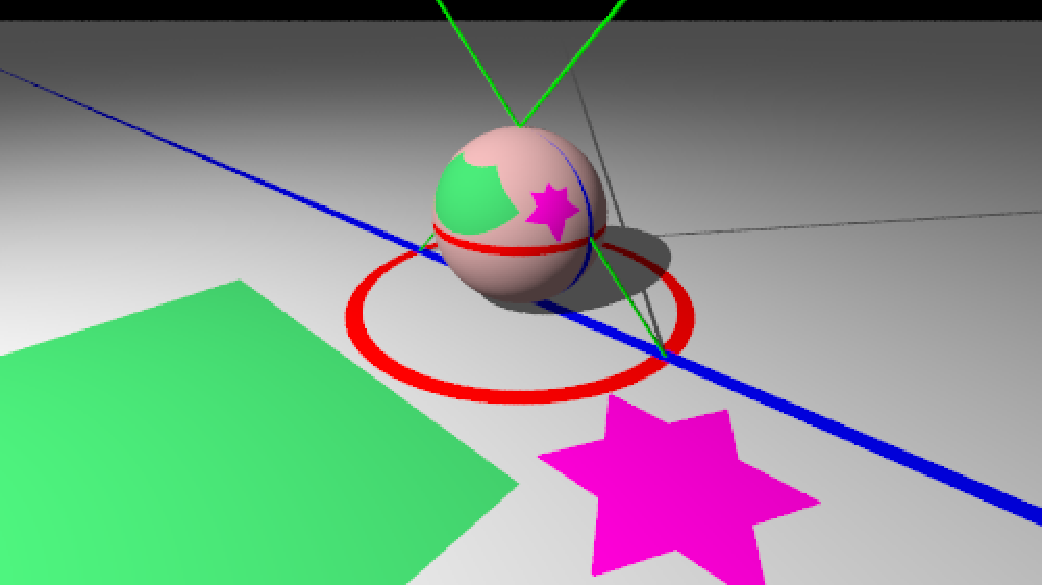
\includegraphics[width=3in, height=3in, keepaspectratio]{../img/klein/stereoProject.pdf}
 \caption{Stereographic Projection}
 \label{fig:stereoProject}
\end{figure}

\begin{figure}[htbp]
 \begin{minipage}{0.5\hsize}
  \center
  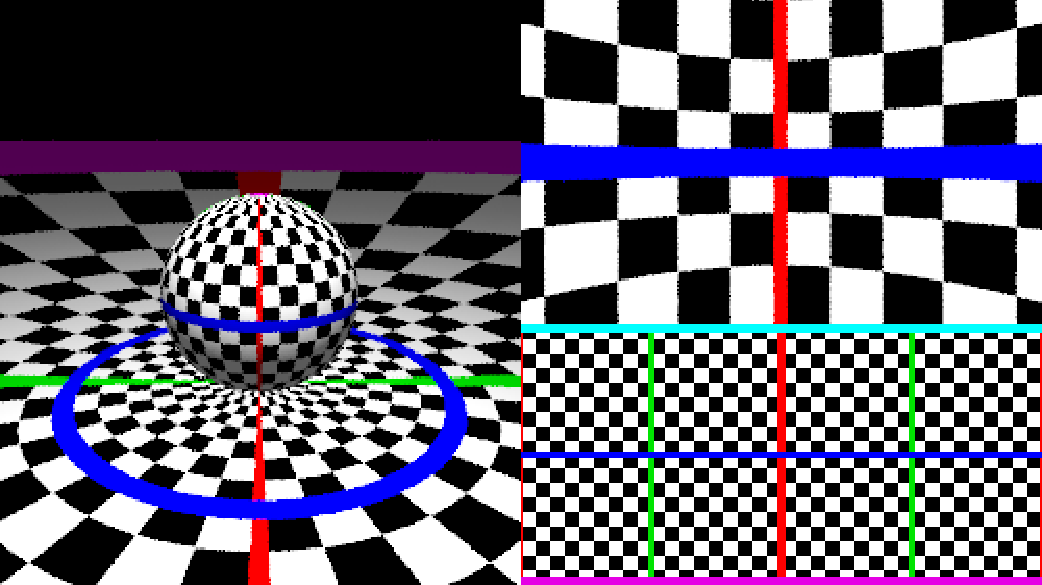
\includegraphics[width=3in, height=3in, keepaspectratio]{../img/klein/spherical.pdf}
  \subcaption{Stereographic }
  \label{fig:sphericalStandard}
 \end{minipage}
 \begin{minipage}{0.5\hsize}
  \center
  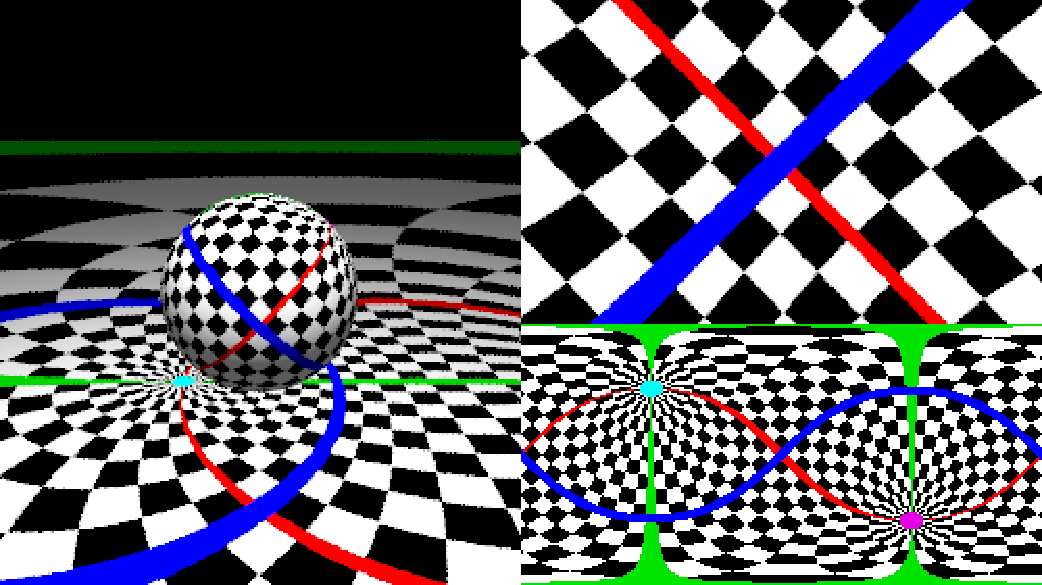
\includegraphics[width=3in, height=3in, keepaspectratio]{../img/klein/sphericalRotation.pdf}
  \subcaption{Rotation}
  \label{fig:sphericalRotation}
 \end{minipage}
 \caption{Spherical image}
 \label{fig:spherical}
\end{figure}

\subsection{Graph Traversal Approach}

この節では木構造の探索によるクライン群の可視化について記述する.
群を構成する変換の全組み合わせを調べるとき,変換の語で構成される木構造を考える.
図\ref{fig:wordTree}のような木はケーリーグラフ(Cayley graph)と呼ばれ4種類の変換の合成の組合せを表わしている.
この木を探索することで得られる合成変換を用いて群の作用を可視化する.
疑似コードを含む詳細な解説は『インドラの真珠』にある.

メビウス変換は4つの複素数で構成されているが, このままでは自由度が高すぎ
るため,群を考えるときにはパラメータ化する.
パラメータ化された式は群の「レシピ」ともよばれる.
例えば, 『インドラの真珠』で使われる「おばあちゃんのレシピ」では, 二つの複素数
$t_a, t_b$をパラメータにとることで, 以下のように2つの生成元を得ることができる.
\begin{enumerate}
 \item 二つの複素数,$t_z, t_b$を選ぶ.
 \item  二次方程式
        $x^2 - t_a t_b x + t_a^2 + t_b^2 = 0 \text{の一方の解}x\text{を
        選び, }t_{ab}= \text{とする. }$
 \item $z_0$を次のように定義する.
       $z_0 = \frac{(t_{ab} -2)t_b}{t_b t_{ab} - 2 t_a + 2it_{ab}}$
 \item 生成元の行列は次のようになる.
        \begin{align*}
       &a = \left(
      \begin{array}{ccc}
       \frac{t_a}{2} & \frac{t_a t_{ab} - 2 t_b + 4i}{(2 t_{ab} + 4)z_0} \\
       \frac{(t_a t_{ab} - 2 t_b -4i)z_0}{2 t_{ab} - 4} & \frac{t_a}{2}
      \end{array}
     \right)\\
 &b = \left(
      \begin{array}{ccc}
       \frac{t_b - 2i}{2} & \frac{t_b}{2} \\
       \frac{t_b}{2} & \frac{t_b + 2i}{2}
      \end{array}
     \right)
        \end{align*}
\end{enumerate}
「おばあちゃんのレシピ」は群を可視化した際に綺麗な図がレンダリングされるように共役によって調整されている.

\begin{figure}[htbp]
 \center
 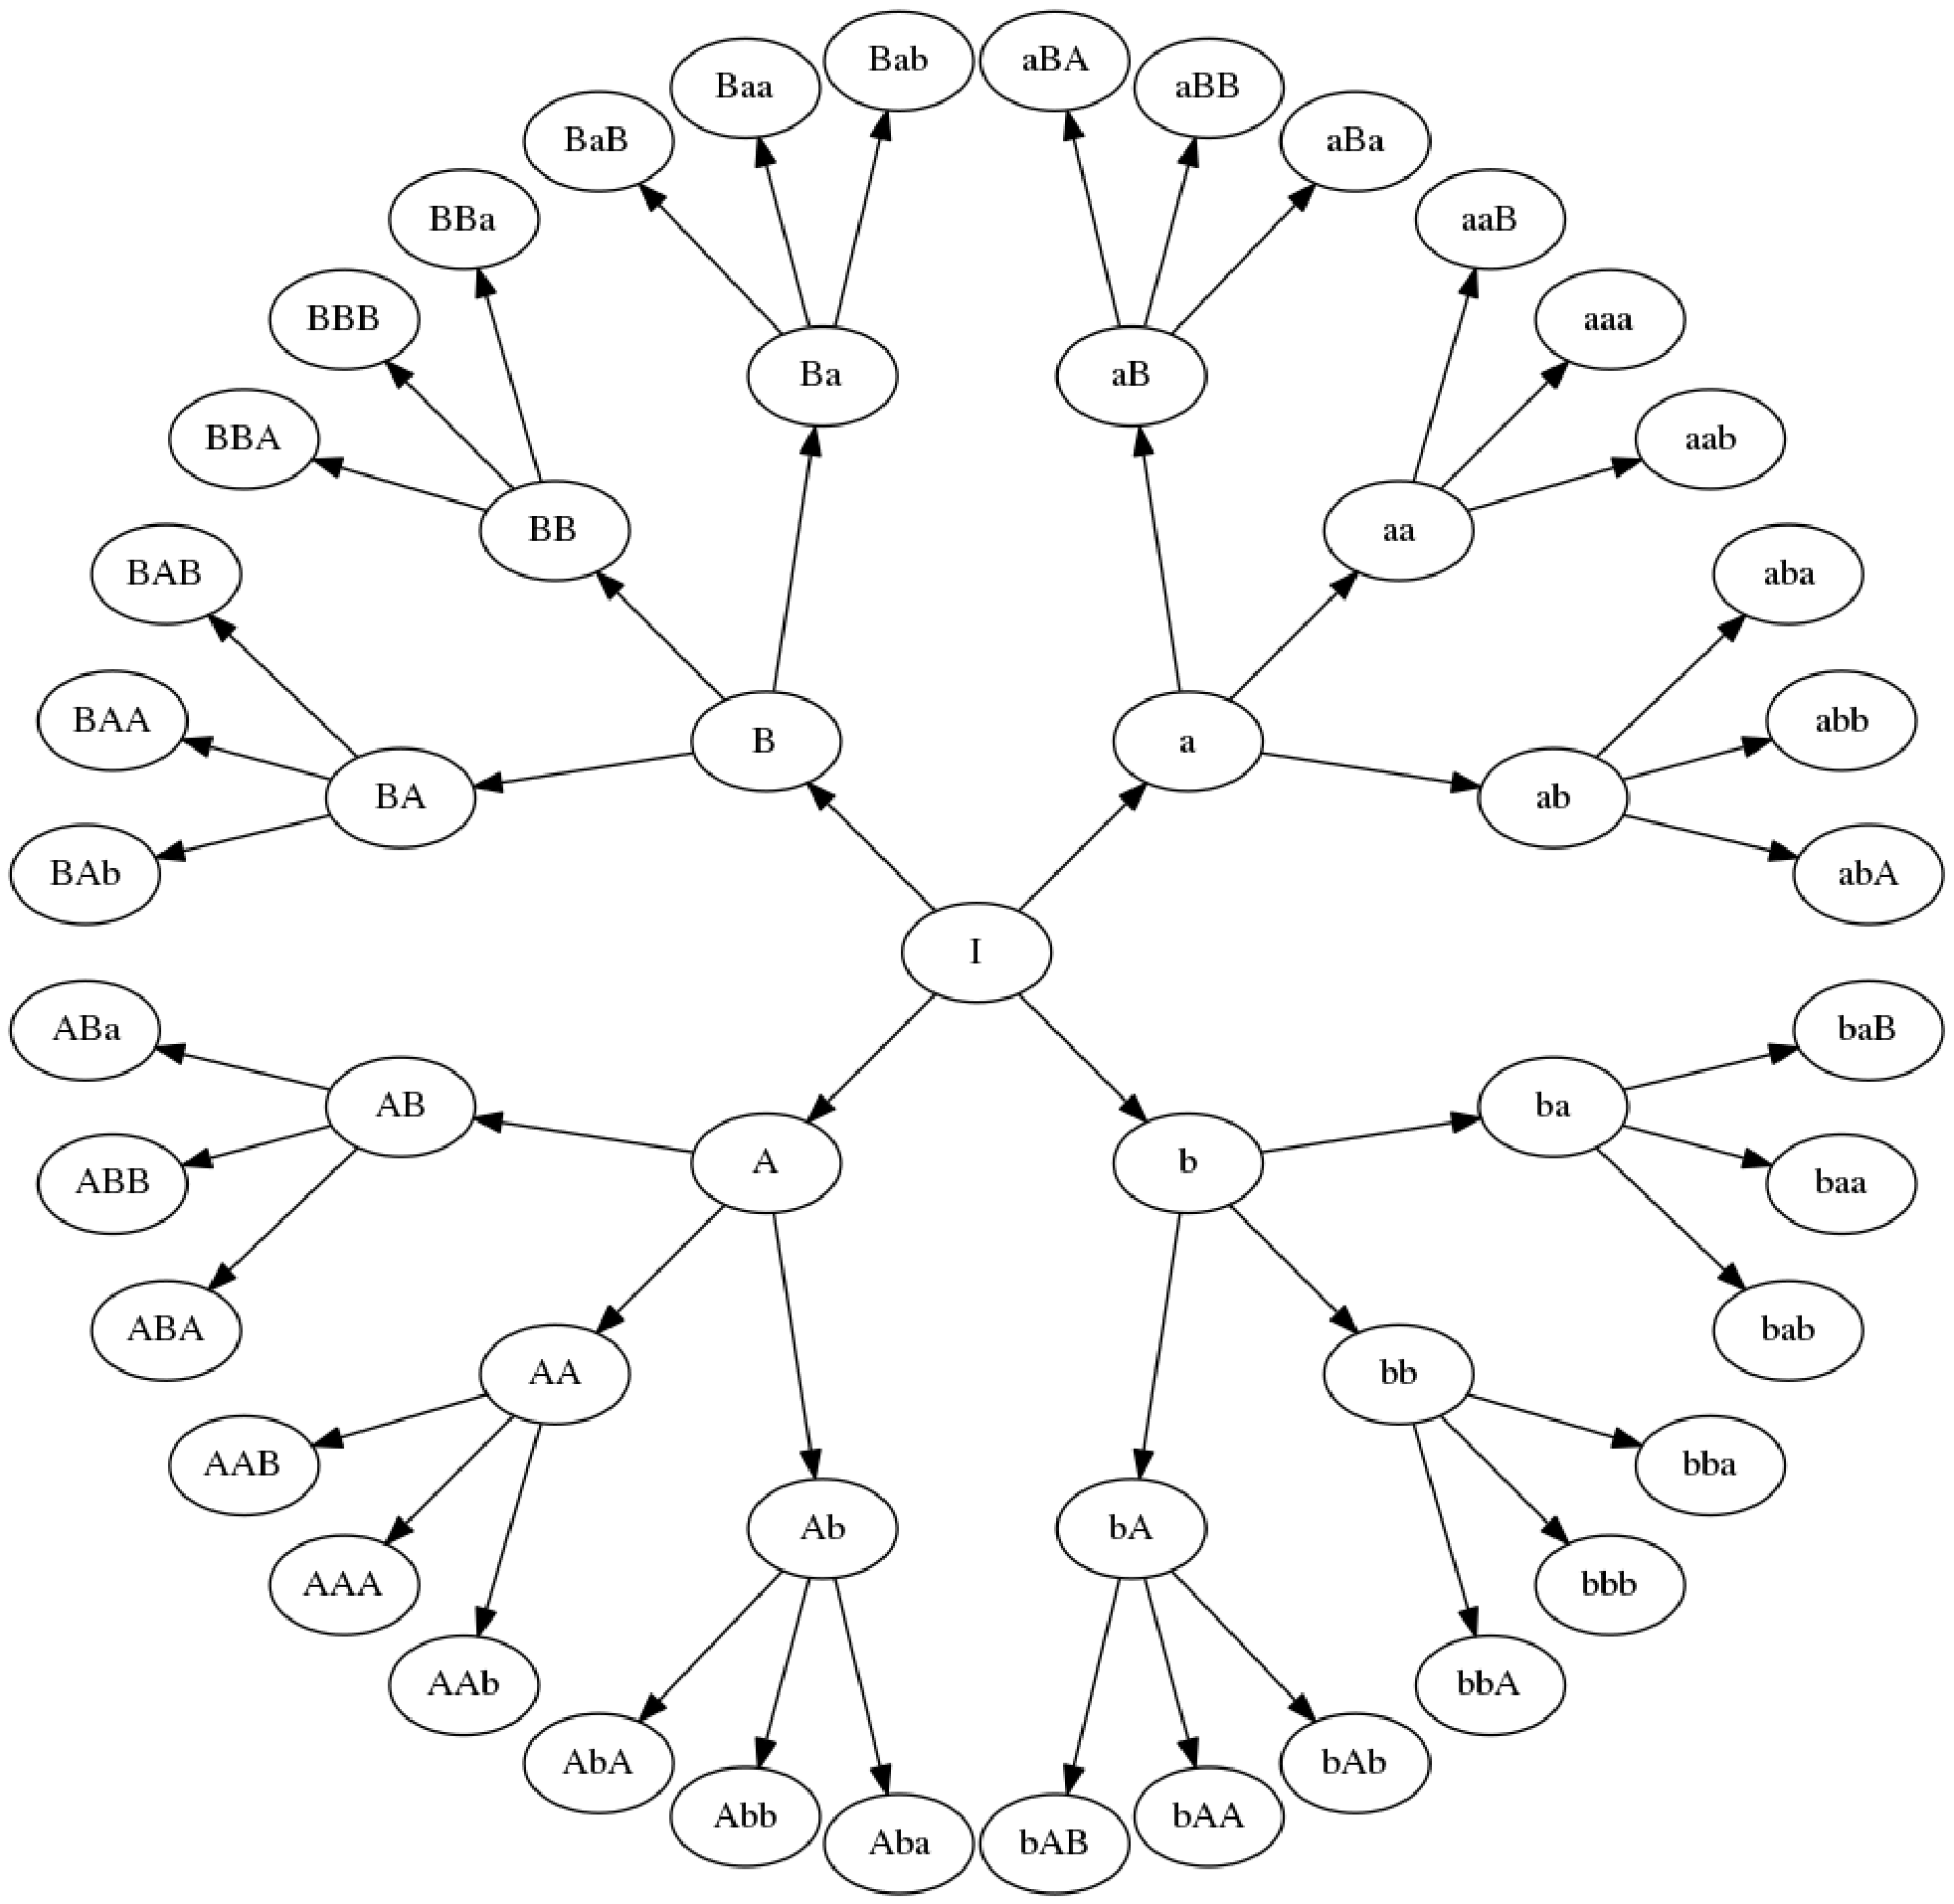
\includegraphics[width=3in, height=3in, keepaspectratio]{../img/klein/wordTree.pdf}
 \caption{Word Tree}
 \label{fig:wordTree}
\end{figure}

\subsubsection{Rendering the Orbit of Transformations}

まず, 円の反転で構成される群を可視化してみよう.
円の反転は変換自体を円という図形で表現できるため, その作用を理解しやすい.
図\ref{fig:schottky}には4つ円の内側にたくさんの円が描かれている.

外側にある4つの大きな円を反転円とよぶ.
それぞれの反転円の反転は自分以外の反転円を自分の内側に移す.
よって,それぞれの反転円に関する反転を行なうと, それぞれの円の内側には3
つの円が移され,合せて12個の小円ができる.
新たにできた小円に対してもその小円が属している反転円以外の反転を適用することで, 小円の下に新たな小円ができる.
このことを繰り返すと,図\ref{fig:schottky}のように,円が入れ子状につらな
る図を得ることができる.
これを反転円の\emph{軌道}とよぶ.
また,円列の極限を極限集合とよぶ.

図\ref{fig:schottky}では反転円の軌道を描いが, 同様にして違う図形の軌道を描くこともできる.
例えば, 図\ref{fig:orbit}は中央に置いた猫の画像を4つ反転円による反転で移した軌道を描いた.

このアルゴリズムは変換で構成される木構造を幅優先探索で探索することに等しい.
例えば, 図\ref{fig:wordTree}の語の木を時計回りに探索すると$a, b, A, B,
aB, aa, ab, ba, bb, ...$の順に合成された変換を得ることができる.
あらかじめ決められた深さまで調べたら, 得られたすべての変換の語を大本とな
る図形(図\ref{fig:orbit}における中央の猫)に対して作用させることで, おお
まかに生成元の作用を調べることができる.

\begin{figure}[htbp]
 \begin{minipage}{0.49\hsize}
  \begin{center}
   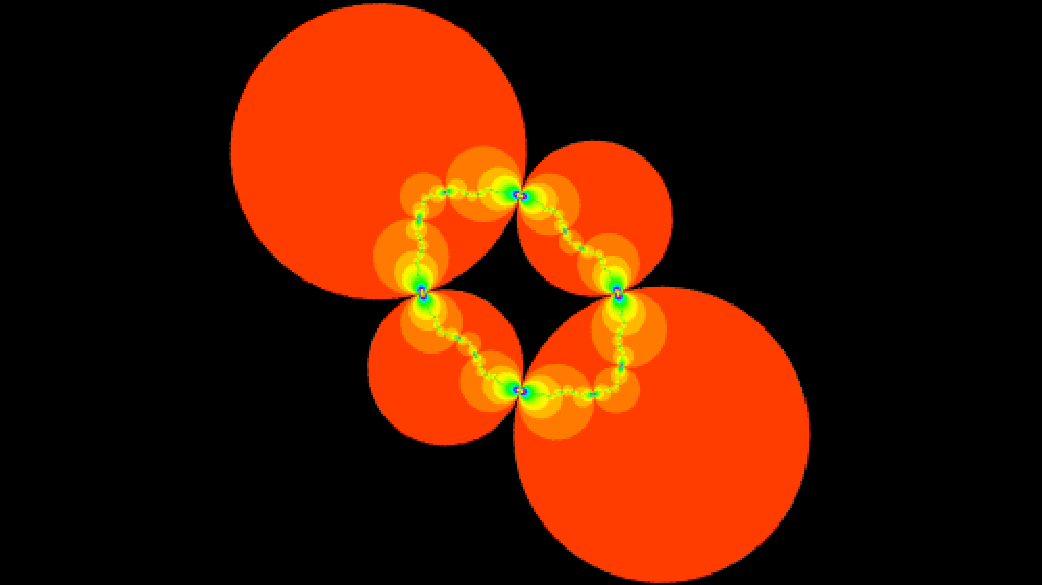
\includegraphics[width=3in, height=3in, keepaspectratio]{../img/klein/schottkyCircles.pdf}
   \caption{Schottky Circles}
   \label{fig:schottky}
  \end{center}
 \end{minipage}
 \begin{minipage}{0.49\hsize}
  \begin{center}
   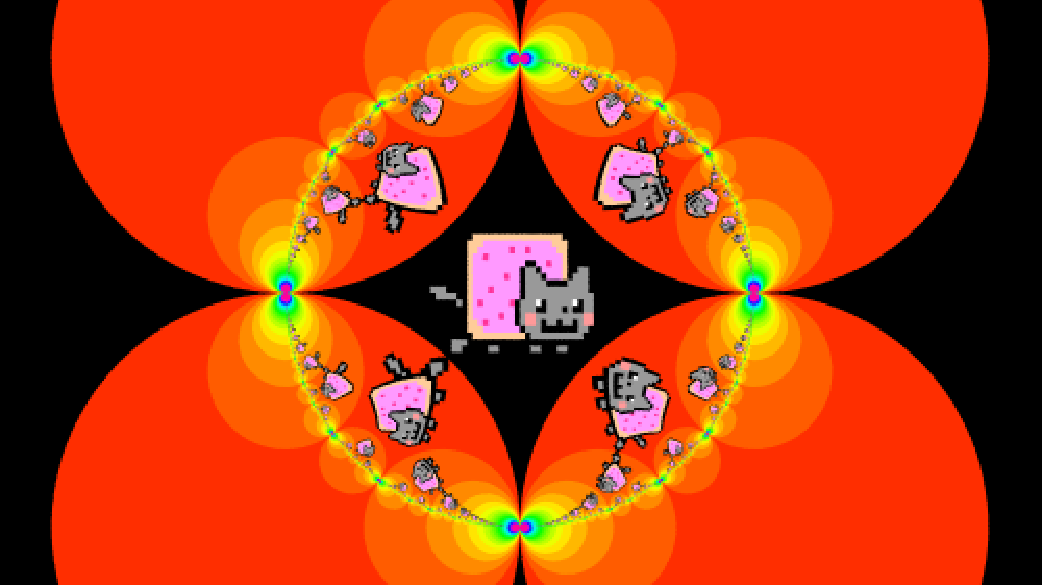
\includegraphics[width=3in, height=3in, keepaspectratio]{../img/klein/circleOrbit.pdf}
   \caption{orbit}
   \label{fig:orbit}
  \end{center}
 \end{minipage}
\end{figure}


\subsubsection{Rendering the Limit Set}

より複雑なメビウス変換群を可視化する際には, 極限集合を直接描く方法が使わ
れる.
極限集合はケーリーグラフにおいて, 無限の深さの語に対応している.
しかし, 現実にそれを求めることは不可能なので, 群の生成元の固定点をある程
度の長さをもった変換の語で移すことで求める.
例えば, 変換$a$の固定点は任意の点に$a$を繰り返し適用した点, つまり
$\overline{a}$を適用した極限点と考えることができる.
例えば, 変換$abbAAb\overline{a}$で表わされる極限点は$a$の固定点を合成変換$abbAAb$で移すことで求めることができる.
この時, $abbAAb$を接頭語と呼ぶ.

図\ref{fig:wordTree}の語の木を時計回りに長さ3までの語を探索すると,$ aBA, aBB, aBa, aaB, ...$という順で接頭語が得られる.
これらの語に, 逆変換をかけないように, 生成元の固定点を与えると極限点を求めることができる.
例えば$aBA$を用いて$\overline{A}, \overline{b}, \overline{B}$の3つの固定点を変換すると互いに近い3つの極限点が得られる.
$aab\overline{a}$と$aaa\overline{a}$のように隣同士の接頭語を持つ極限点や
$aaa\overline{a}$と$aaa\overline{b}$のような同じ接頭語を持つ極限点同士は
近い.
そのため, 得られた点同士を順番に結ぶと図のようなフラクタル構造を持つ曲線を得ることができる.
実際に実装する場合には, 得られた点同士の距離によってより深い語への探索の打ち切りと継続を決める.

図\ref{fig:apr}はP.Nylander氏による作品\footnote{bugman123.com Fractals:
\url{http://bugman123.com/Fractals/index.html}}を参考に描画した.
中央右側の蝶をおばあちゃんのレシピで得られた群の生成元で移した.
虹色の曲線は極限集合である.
どちらの図も図形の軌道は最終的に極限集合へと収束していくことがわかる.

ただし, 綺麗に描画するには様々な工夫が必要となる.
まず, 放物型変換は固定点への収束に時間がかかため, 放物型変換の固定点付近
をうまく描画するためには, 放物型の生成元のための特別な処理が必要である.
図\ref{fig:apr}の右端をよく見ると直線で結ばれていることがわかる.
ここには放物型変換の固定点が存在しており, 収束が遅いため, この近辺の極限点を得るためには, より長い接頭語が必要となっている.
インドラの真珠では特殊語アルゴリズムと呼ばれるアルゴリズムでこの問題に対処する.

また, ある変換に対してその逆変換をかけてしまうと元にもどってしまうことは
自明であるが, 特定の変換の組み合わせが逆戻りを生み出してしまうことがある.
例えば, 先に述べた平行移動の例において,abABという変換は点を一周させて元の場所に戻してしまう.
このような変換をもたない群を\emph{自由群}と呼ぶ.
効率よく描画するためには,逆戻りを生み出す元を取り除く必要がある.
そのためには有限オートマトンが使われる.
有限オートマトンに関する書籍には『Word Processing In Groups』\cite{wordProcessing}がある.

先に述べたように,メビウス変換の群すべてがクライン群になるわけではない.
群の中には描画すると極限集合が収束せず,図\ref{fig:non-discrete}のように
乱れるものがある.
このような群は\emph{非離散群}と呼ばれ,クライン群ではない.
この離散と非離散のパラメータ領域を描画した図は\emph{スライス}と呼ばれ,
スライスの離散と非離散の境界もフラクタル形状となる.
境界付近のパラメータを用いて描画するとしばしば極限集合が興味深い形になる.
山下靖氏のページ\footnote{Discreteness Locus:
\url{http://vivaldi.ics.nara-wu.ac.jp/~yamasita/Slice/}}では様々なスライ
スを見ることができる.
どのようなパラメータが離散的であるか,すなわちクライン群となるかを調べることがクライン群の研究テーマの一つとなる.

\begin{figure}[htbp]
 \begin{minipage}{0.5\hsize}
  \center
  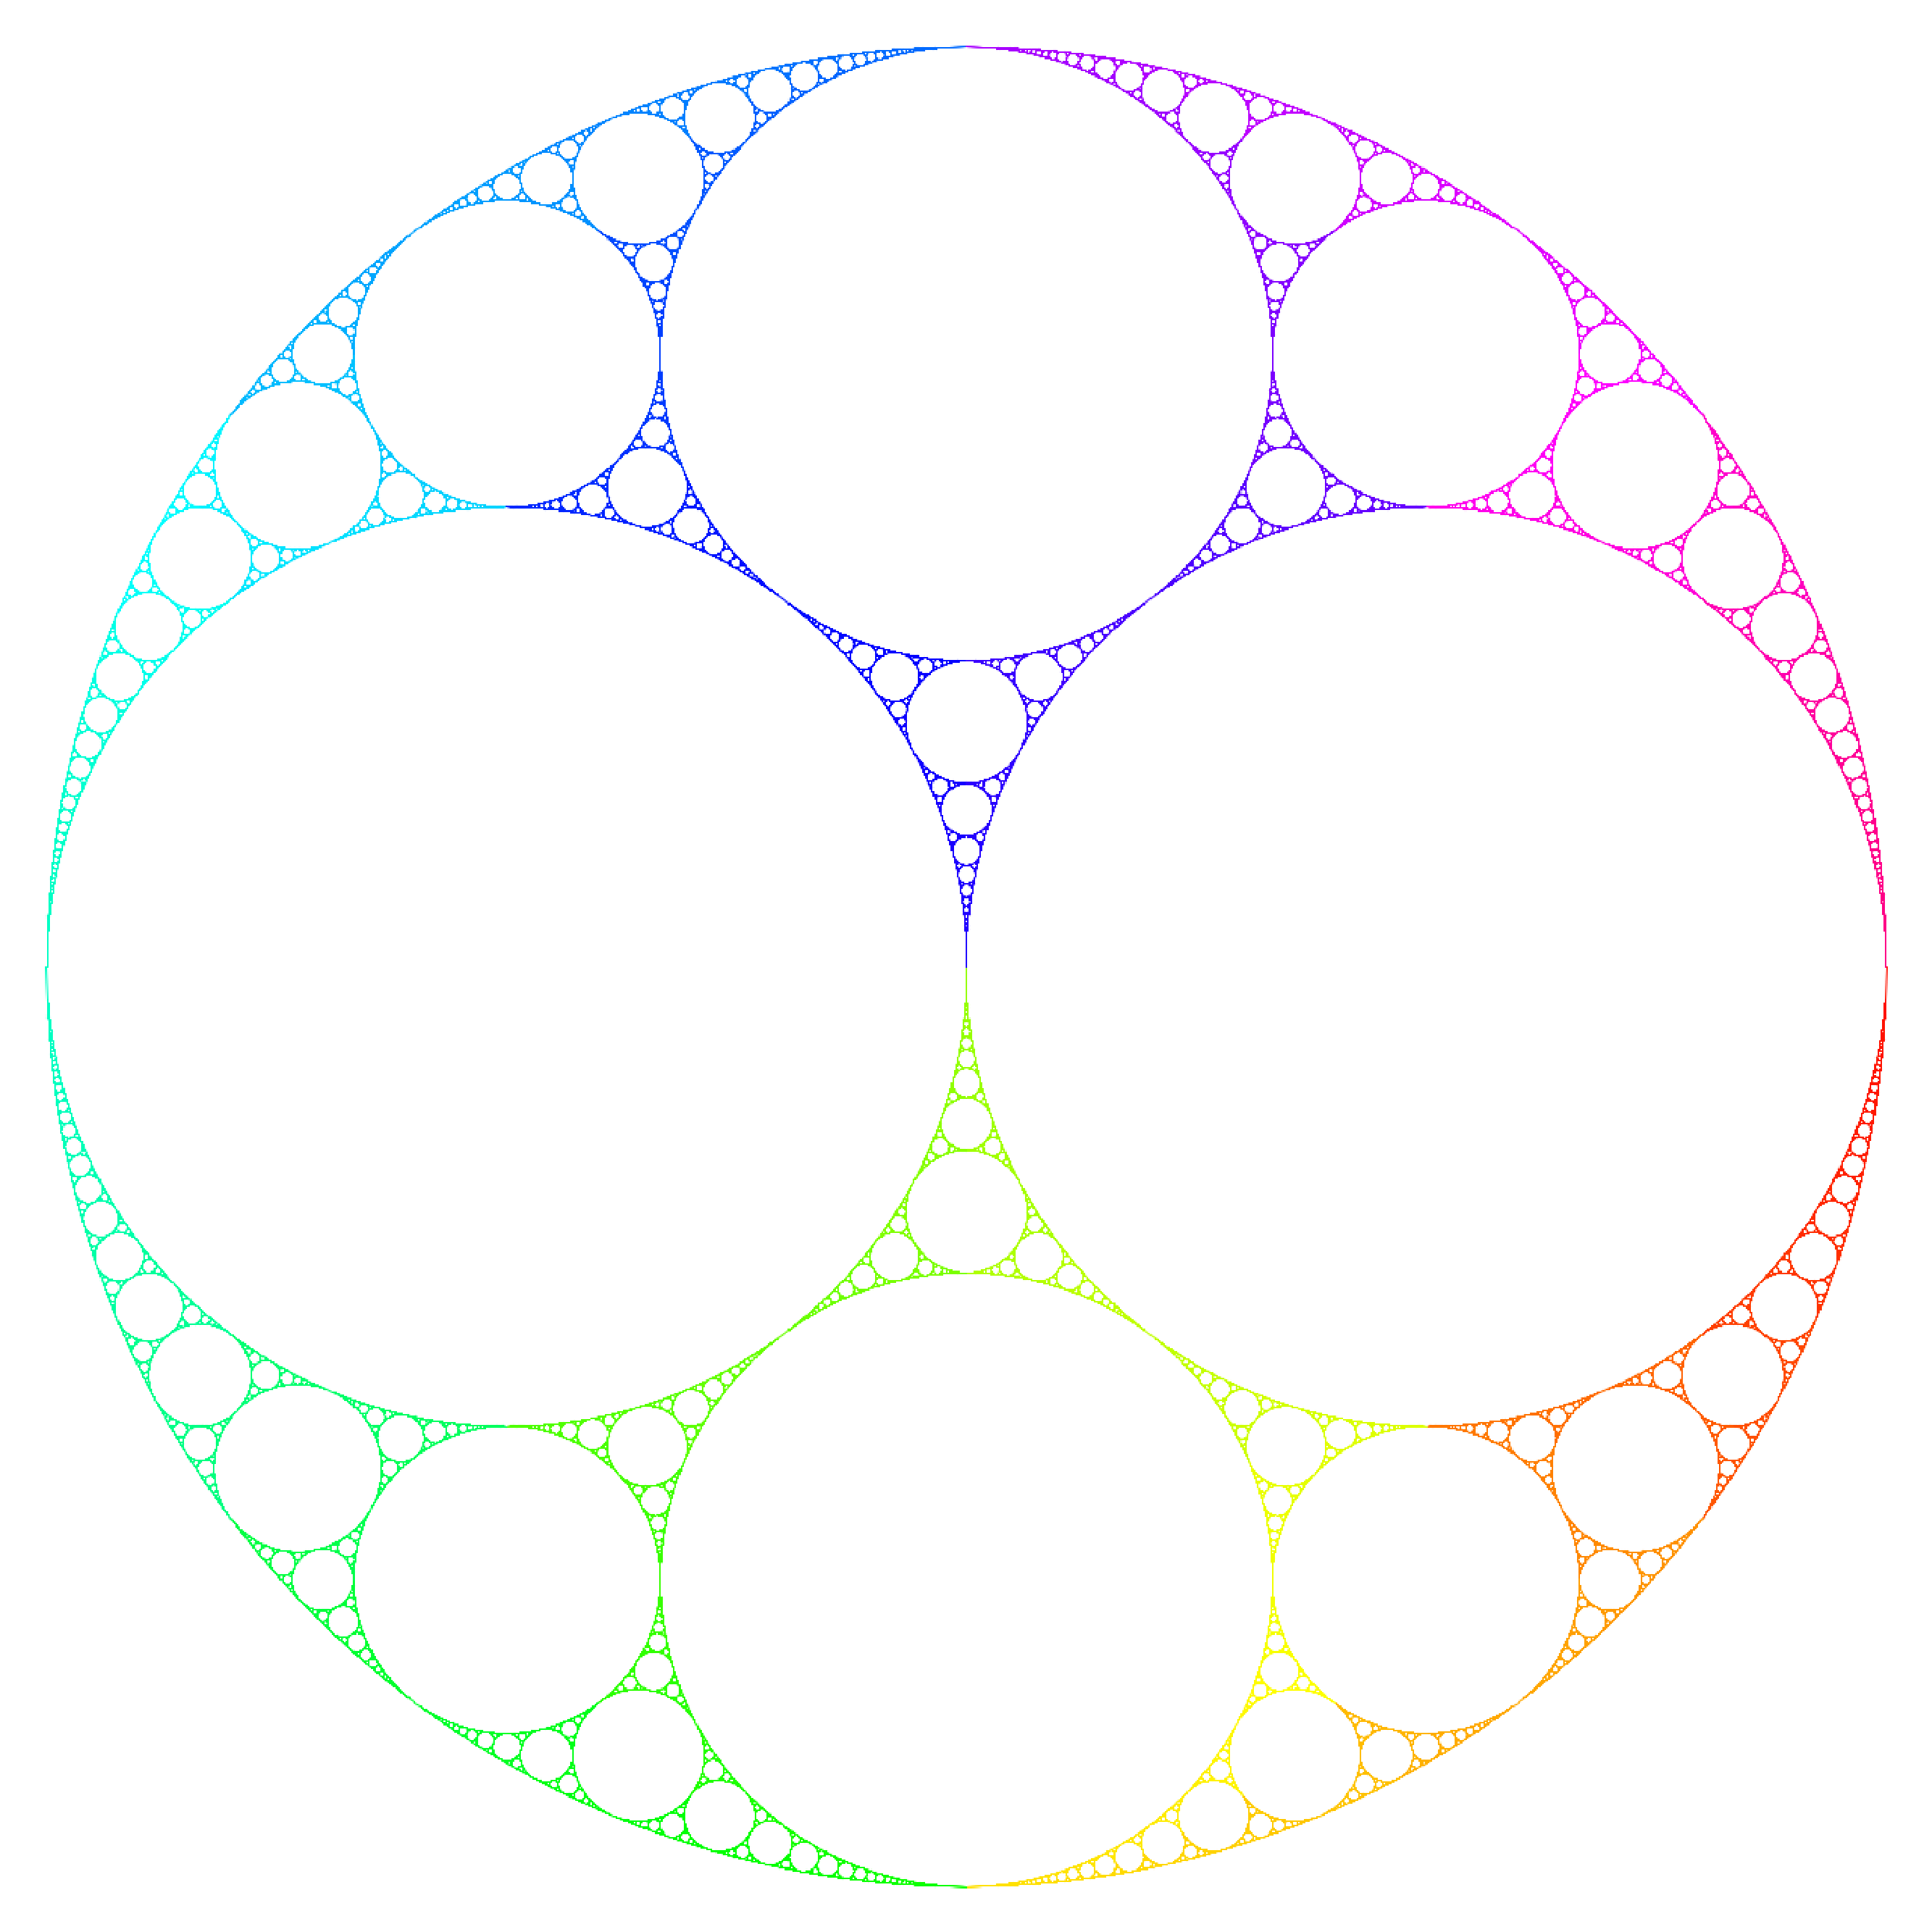
\includegraphics[ height=2.5in, keepaspectratio]{../img/klein/limitset/limit1.pdf}
  \subcaption{}
 \end{minipage}
 \begin{minipage}{0.5\hsize}
  \center
  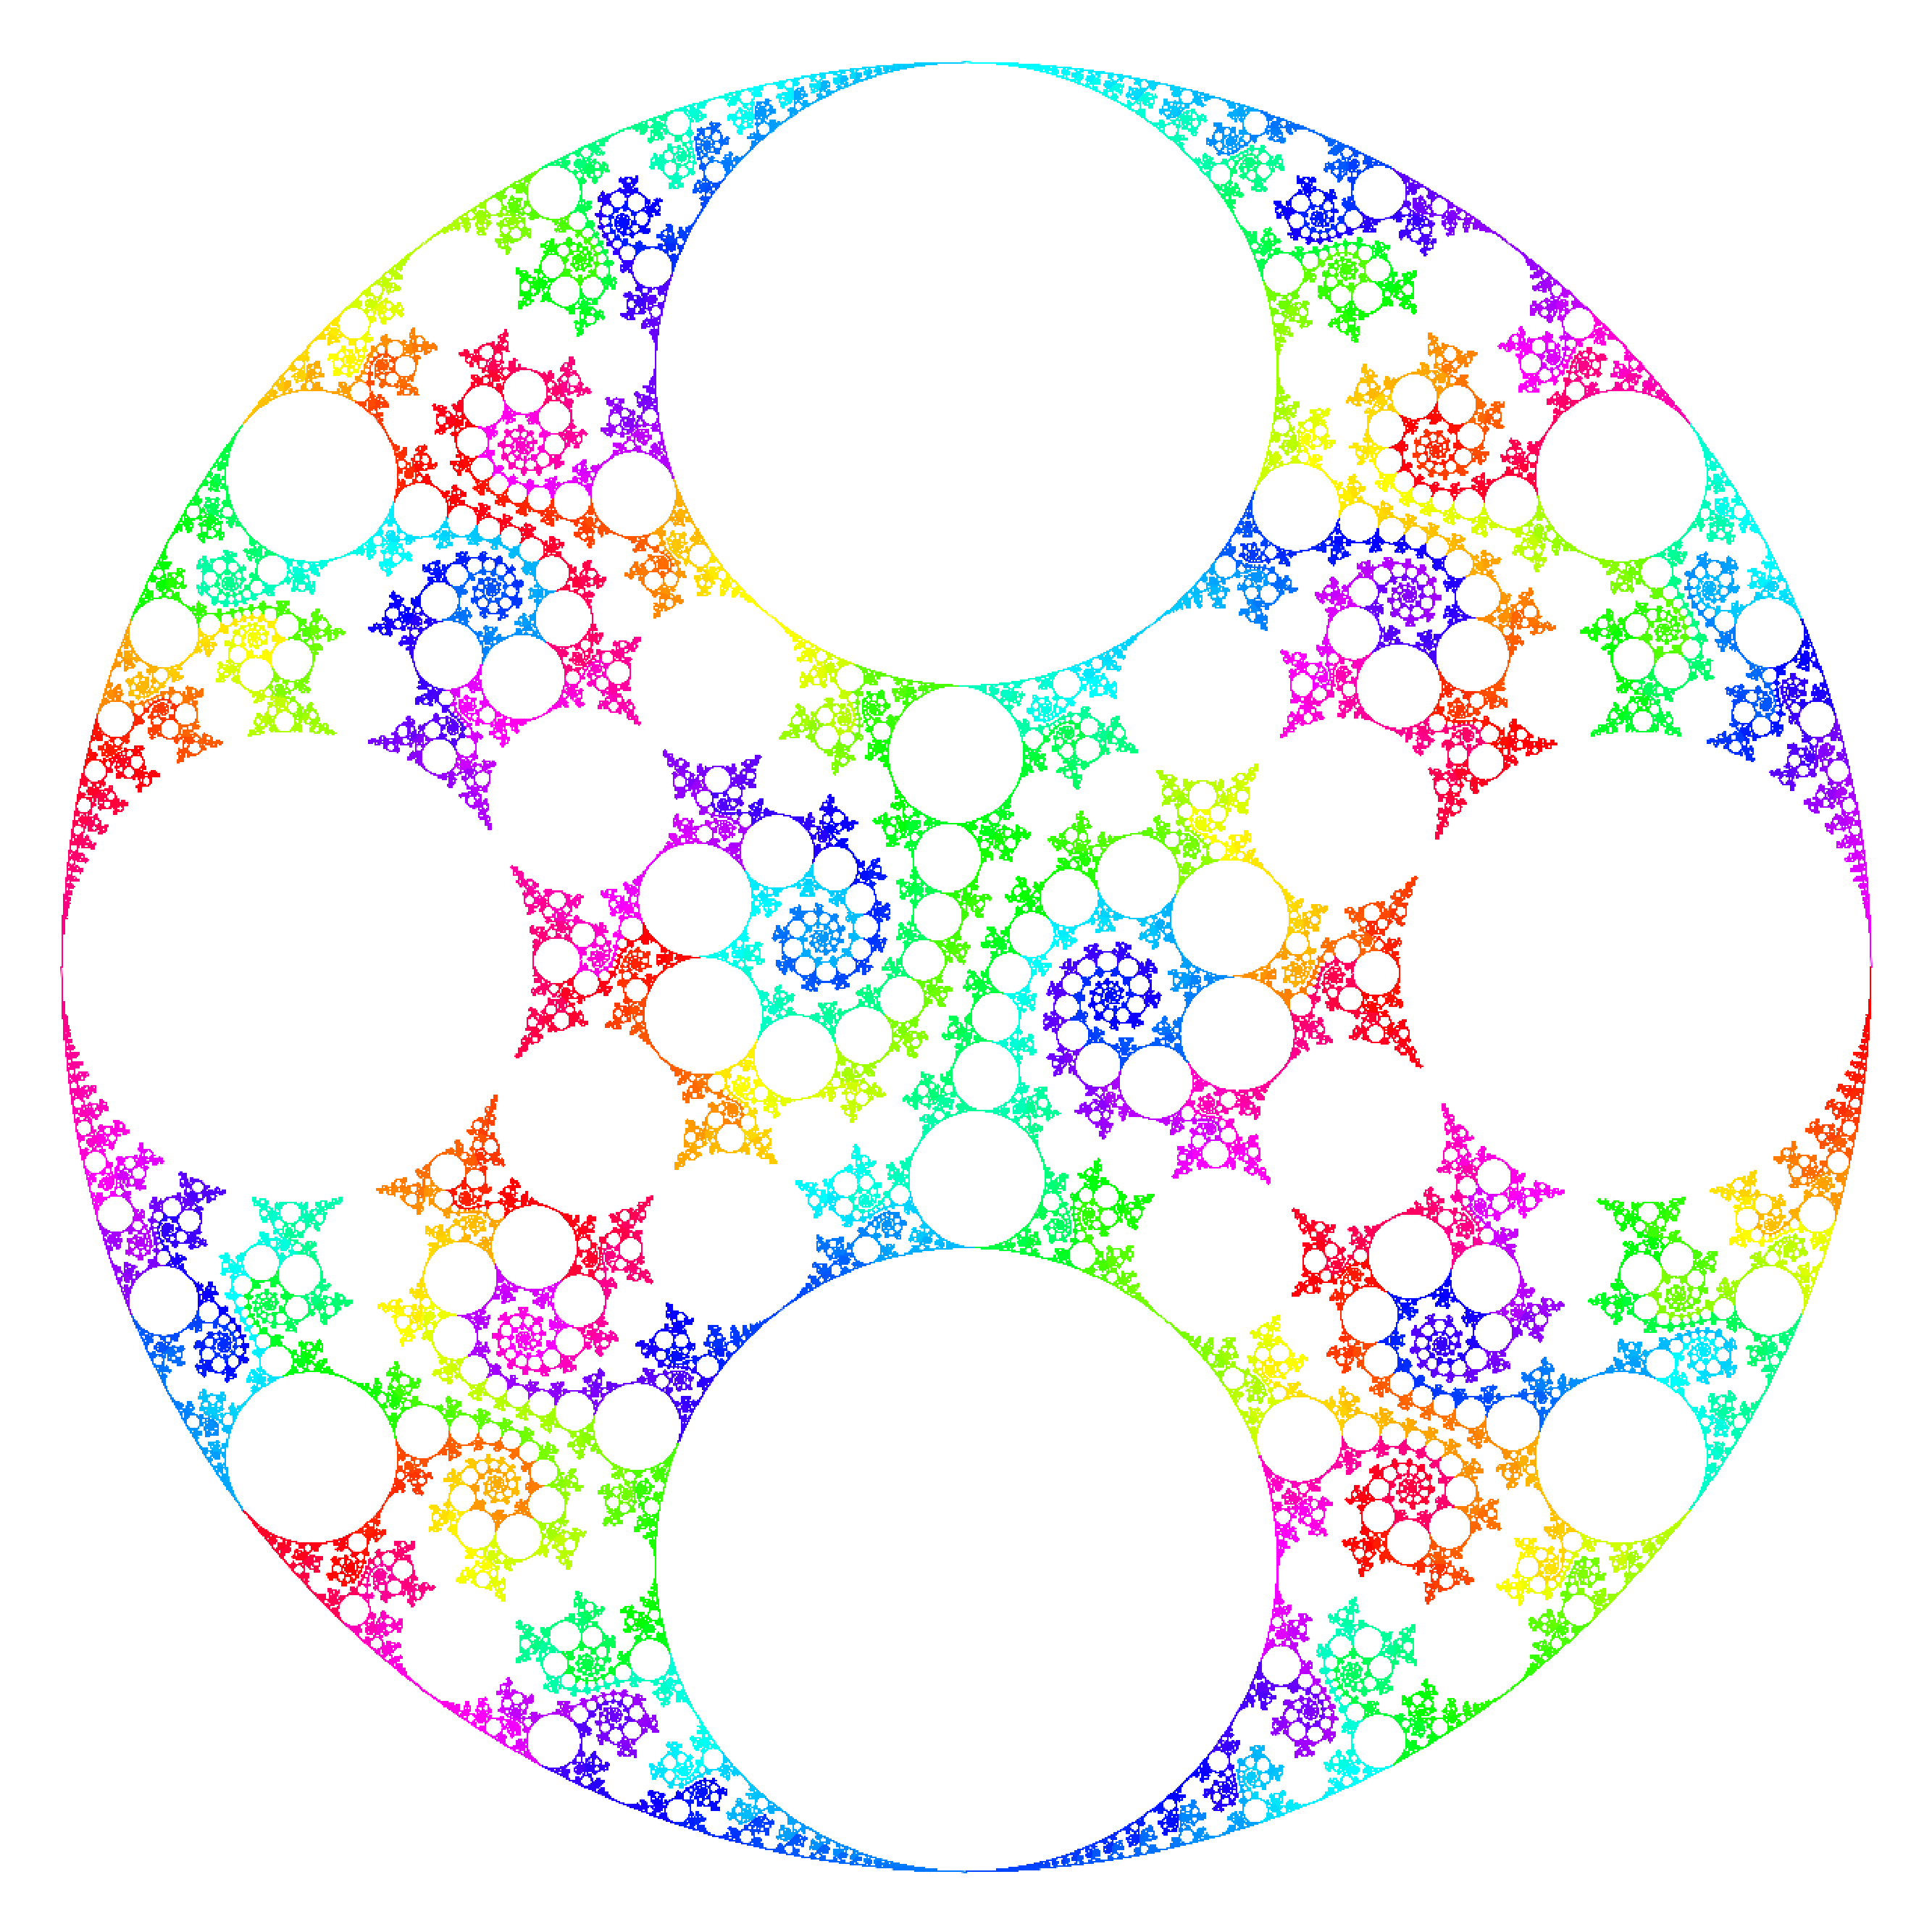
\includegraphics[ height=2.5in, keepaspectratio]{../img/klein/limitset/limit2.pdf}
  \subcaption{}
 \end{minipage}
 \begin{minipage}{0.5\hsize}
  \center
  
\includegraphics[ height=2.5in, keepaspectratio]{../img/klein/limitset/limit3.pdf}
  \subcaption{}
 \end{minipage}
 \begin{minipage}{0.5\hsize}
  \center
  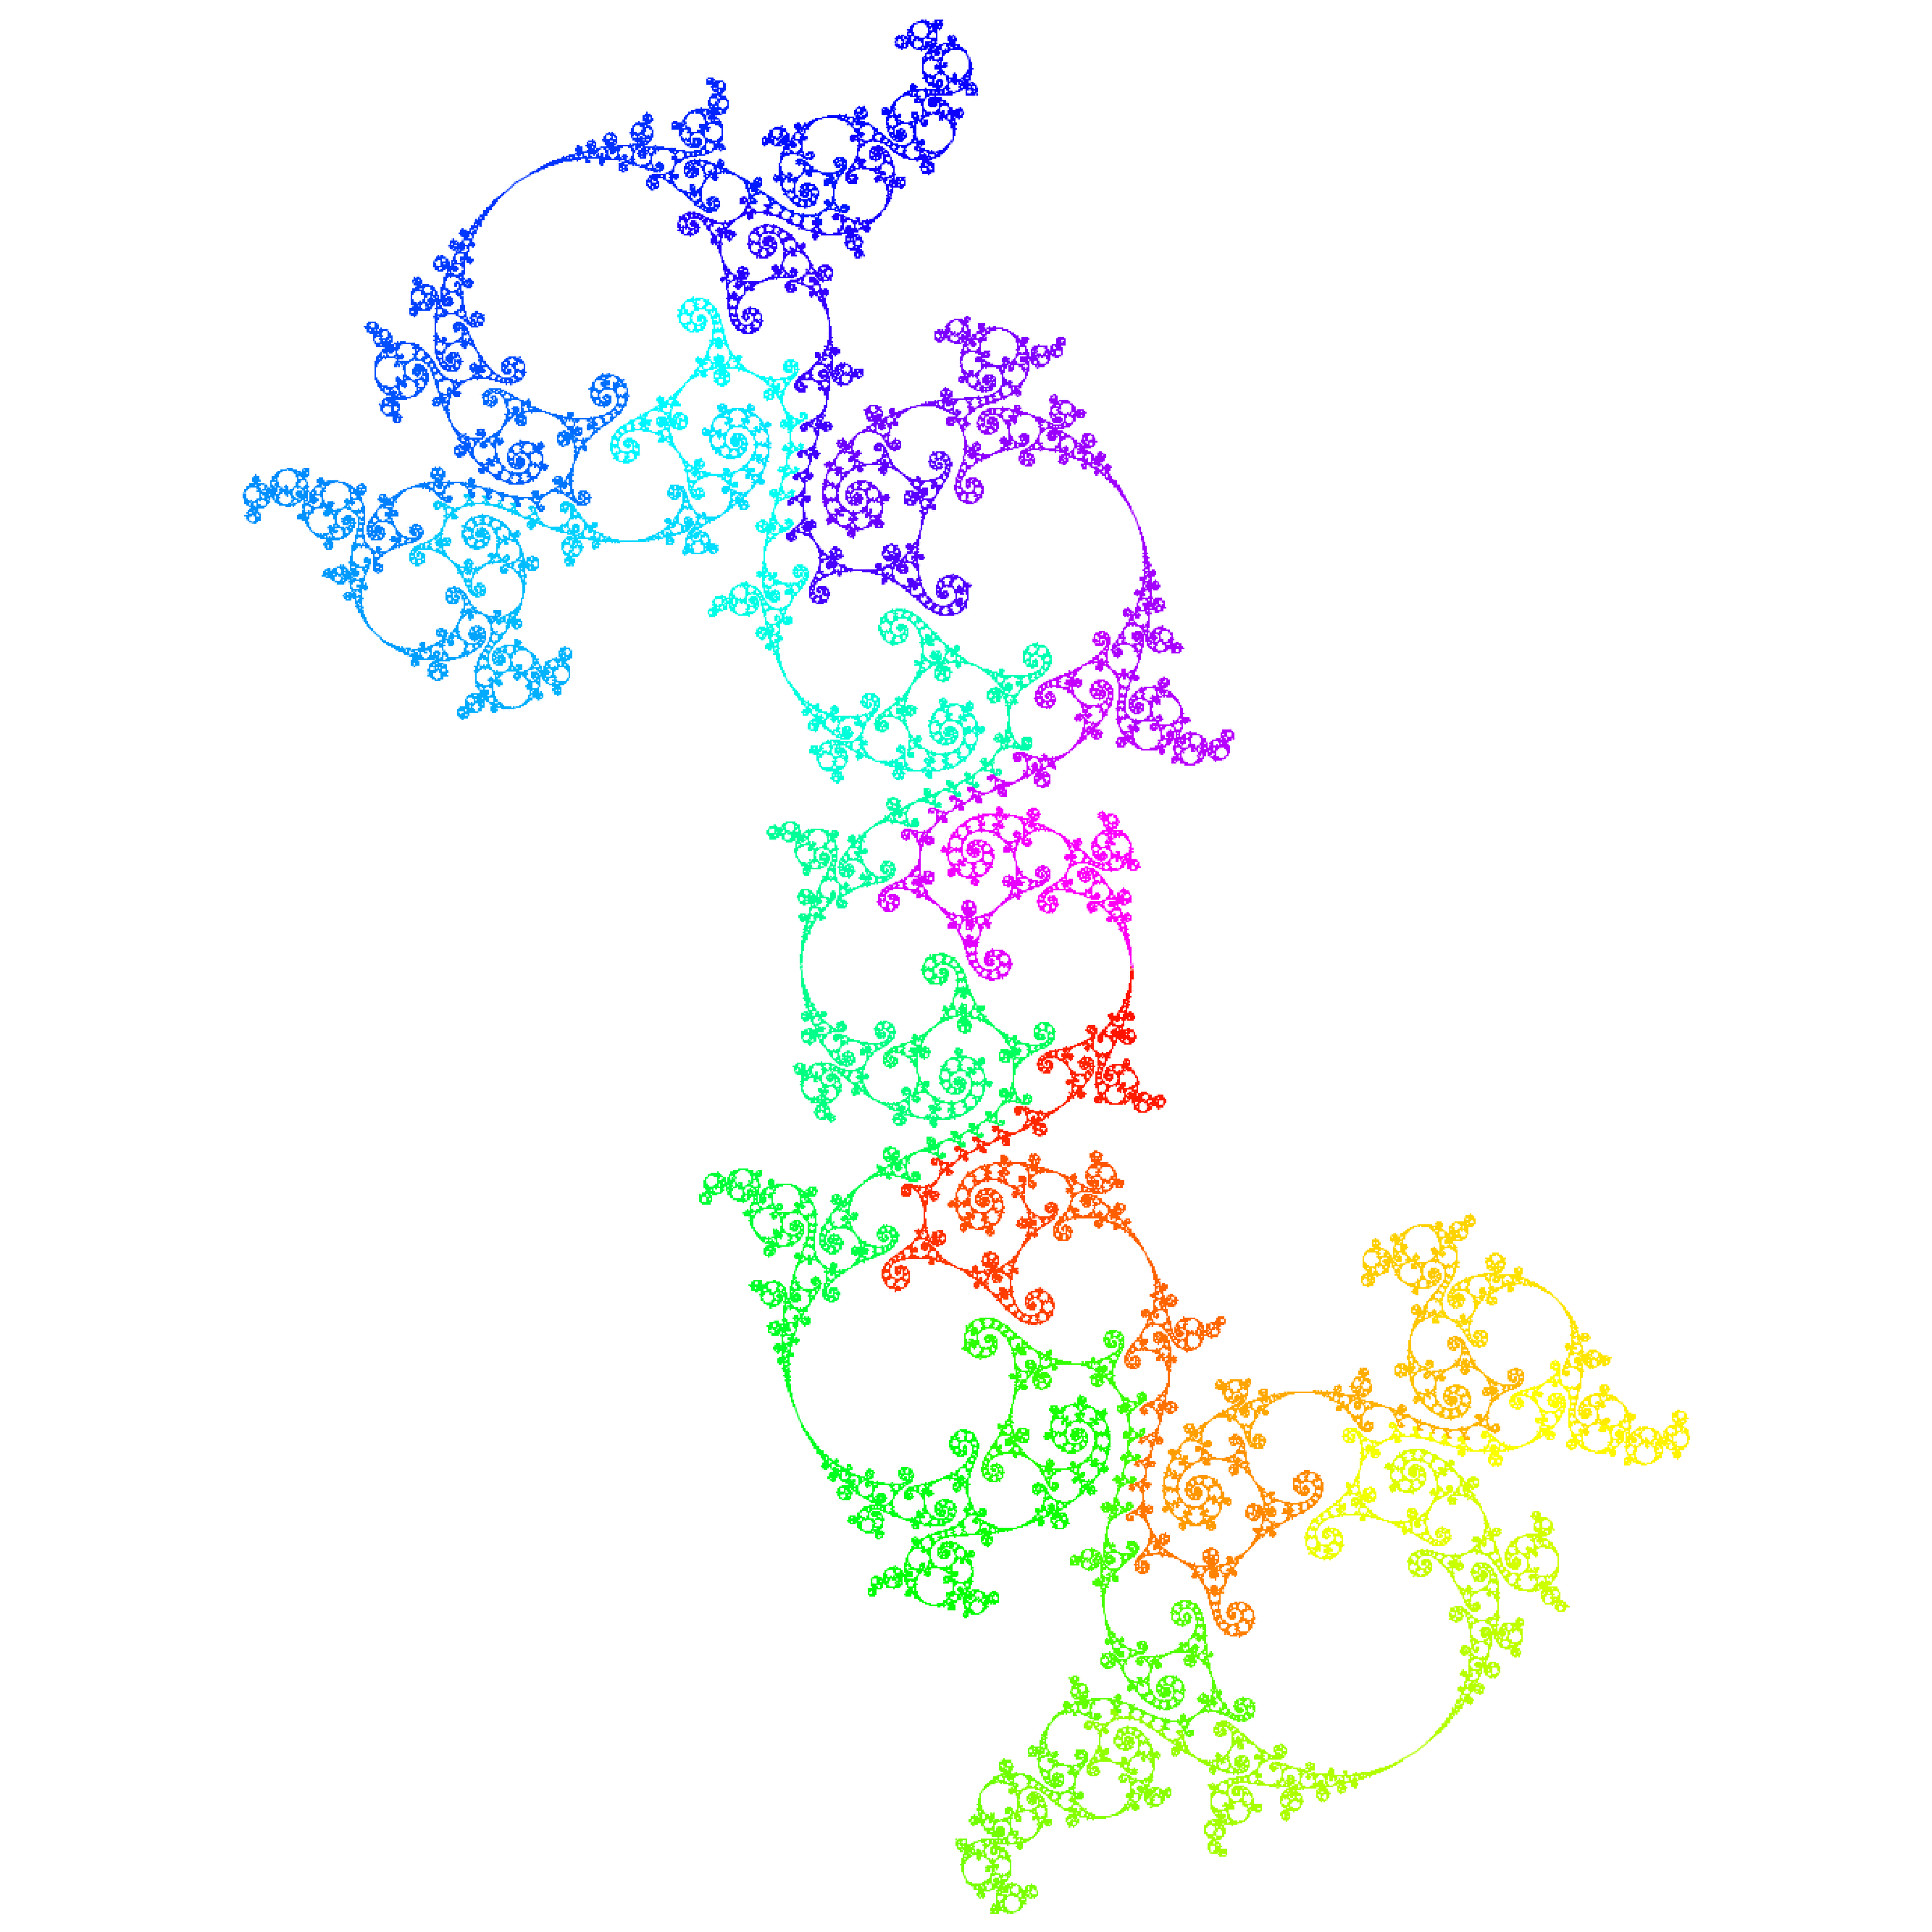
\includegraphics[ height=2.5in, keepaspectratio]{../img/klein/limitset/limit4.pdf}
  \subcaption{}
 \end{minipage}
 \caption{The limit set of Kleinian groups}
\end{figure}

\begin{figure}[htbp]
 \begin{minipage}{0.5\hsize}
  \center
  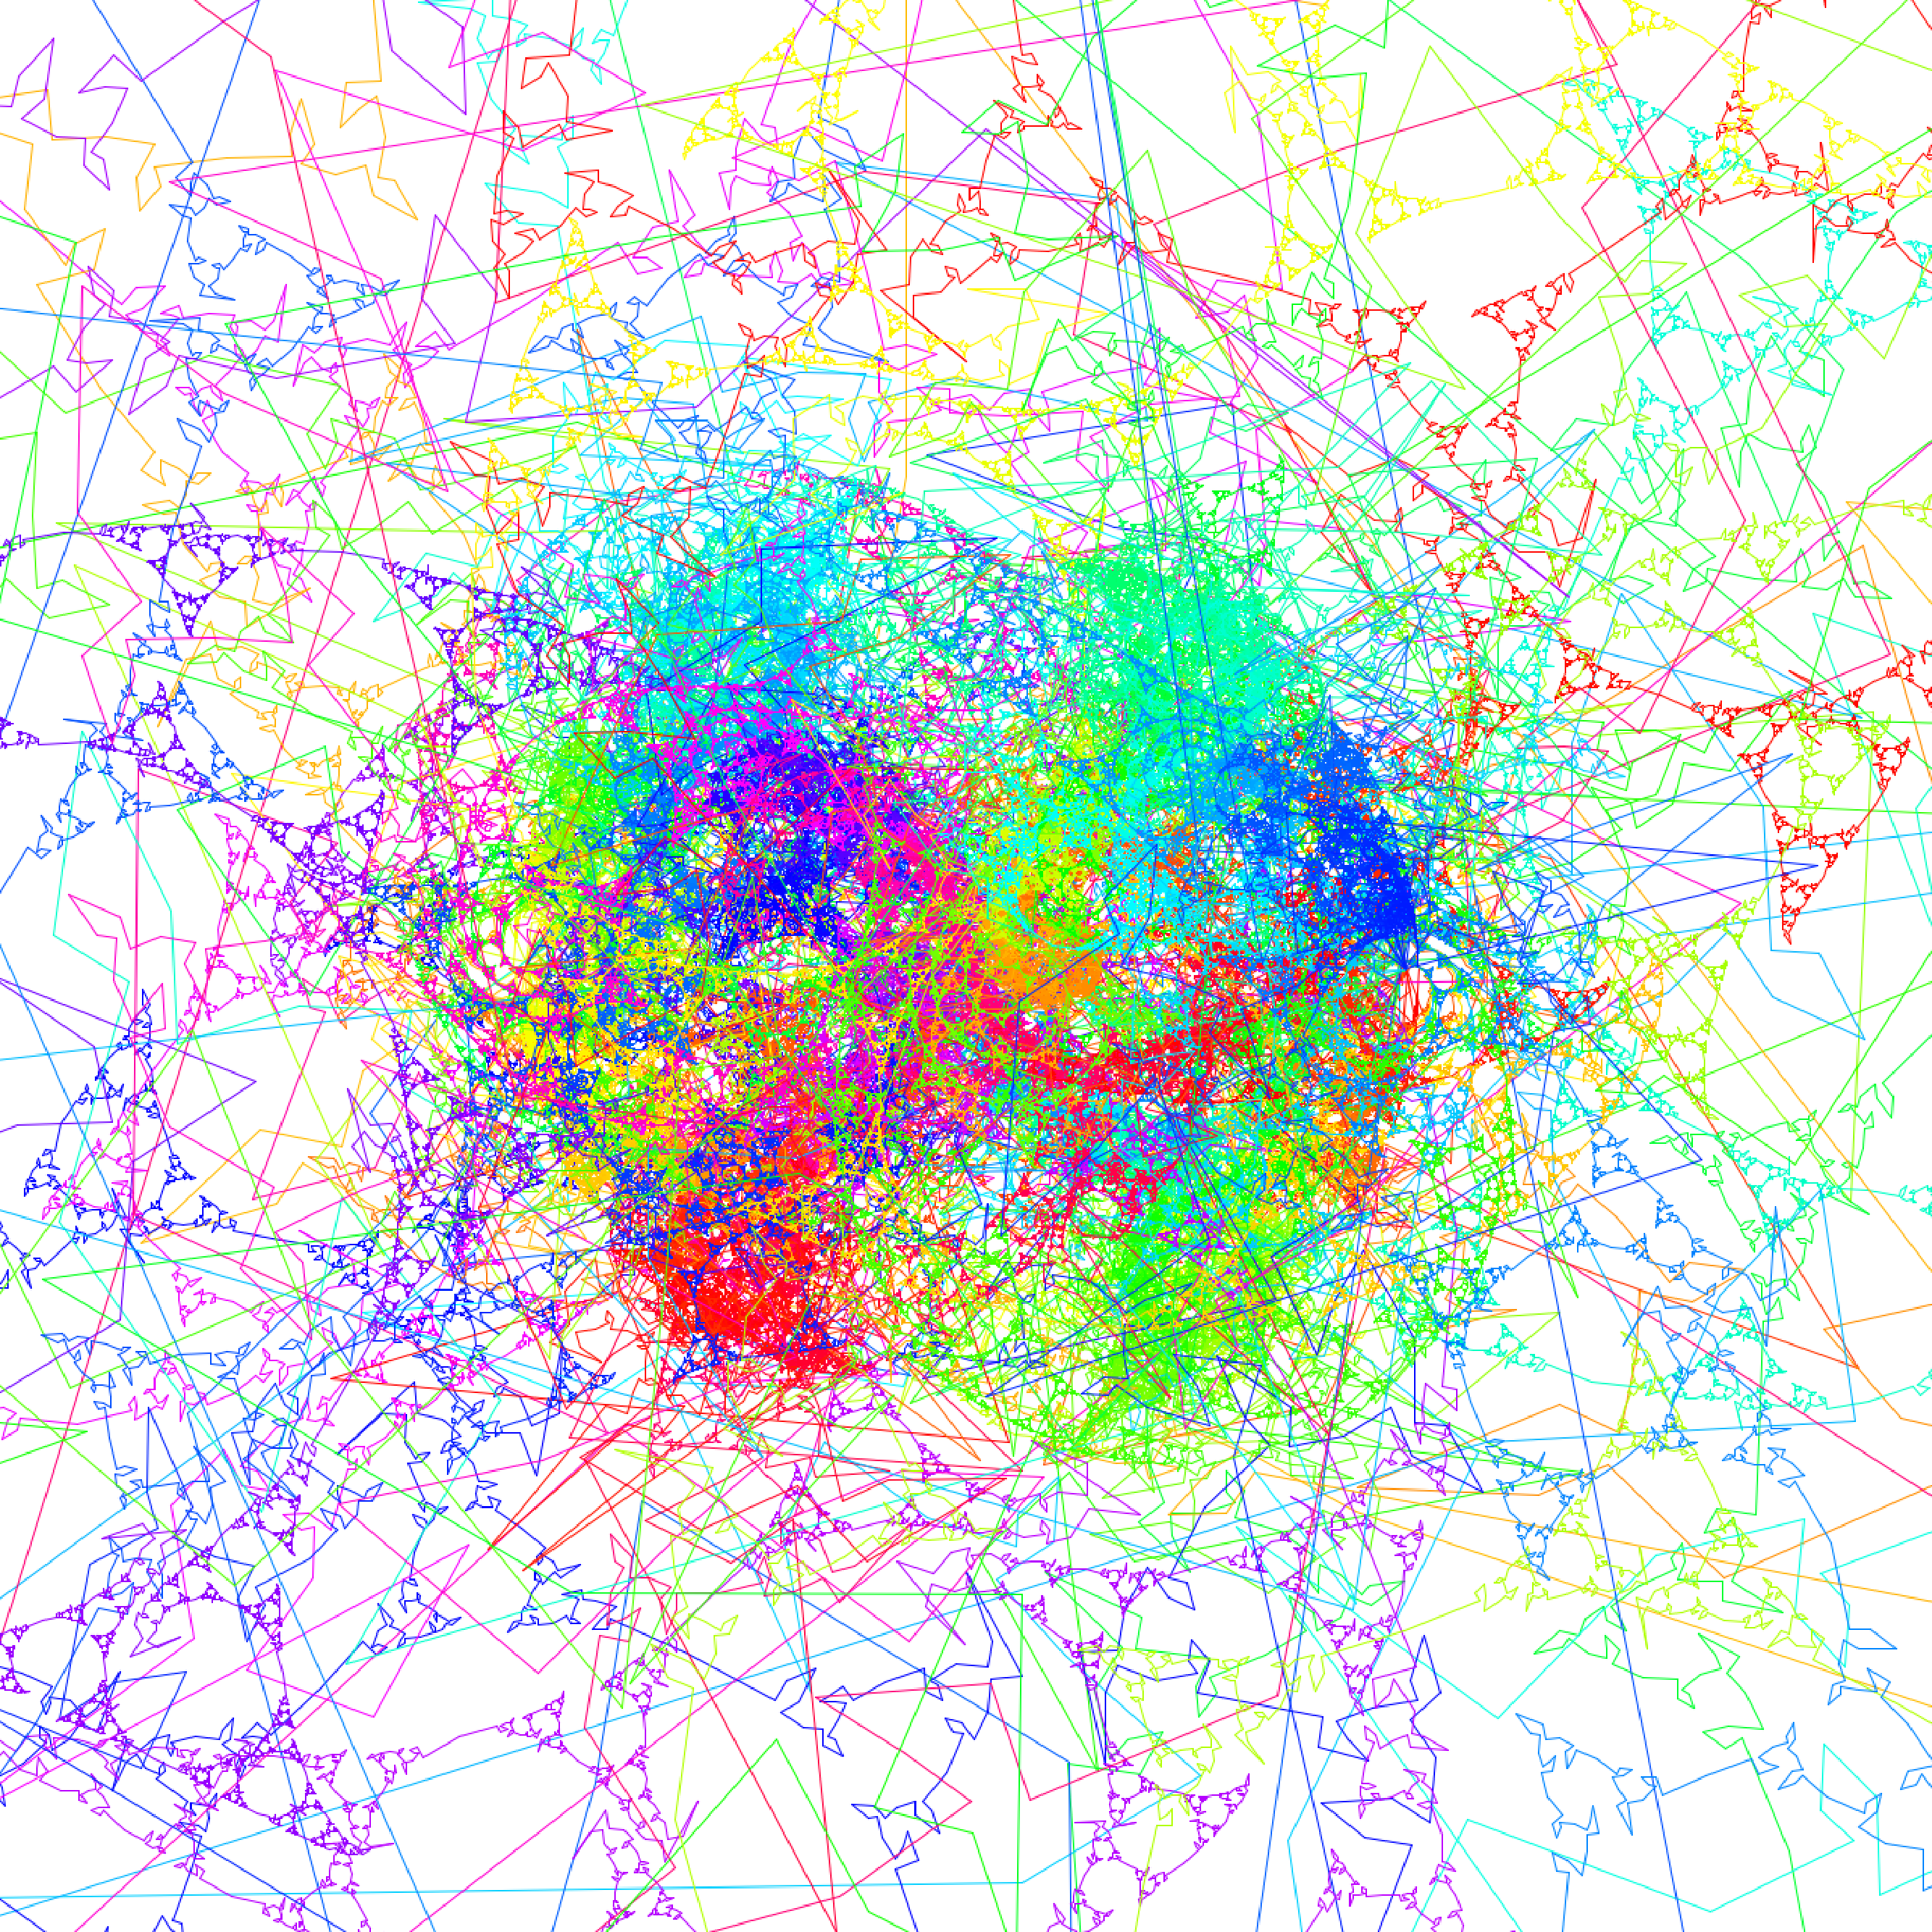
\includegraphics[ height=2.5in, keepaspectratio]{../img/klein/limitset/non-discrete1.pdf}
  \subcaption{}
 \end{minipage}
 \begin{minipage}{0.5\hsize}
  \center
  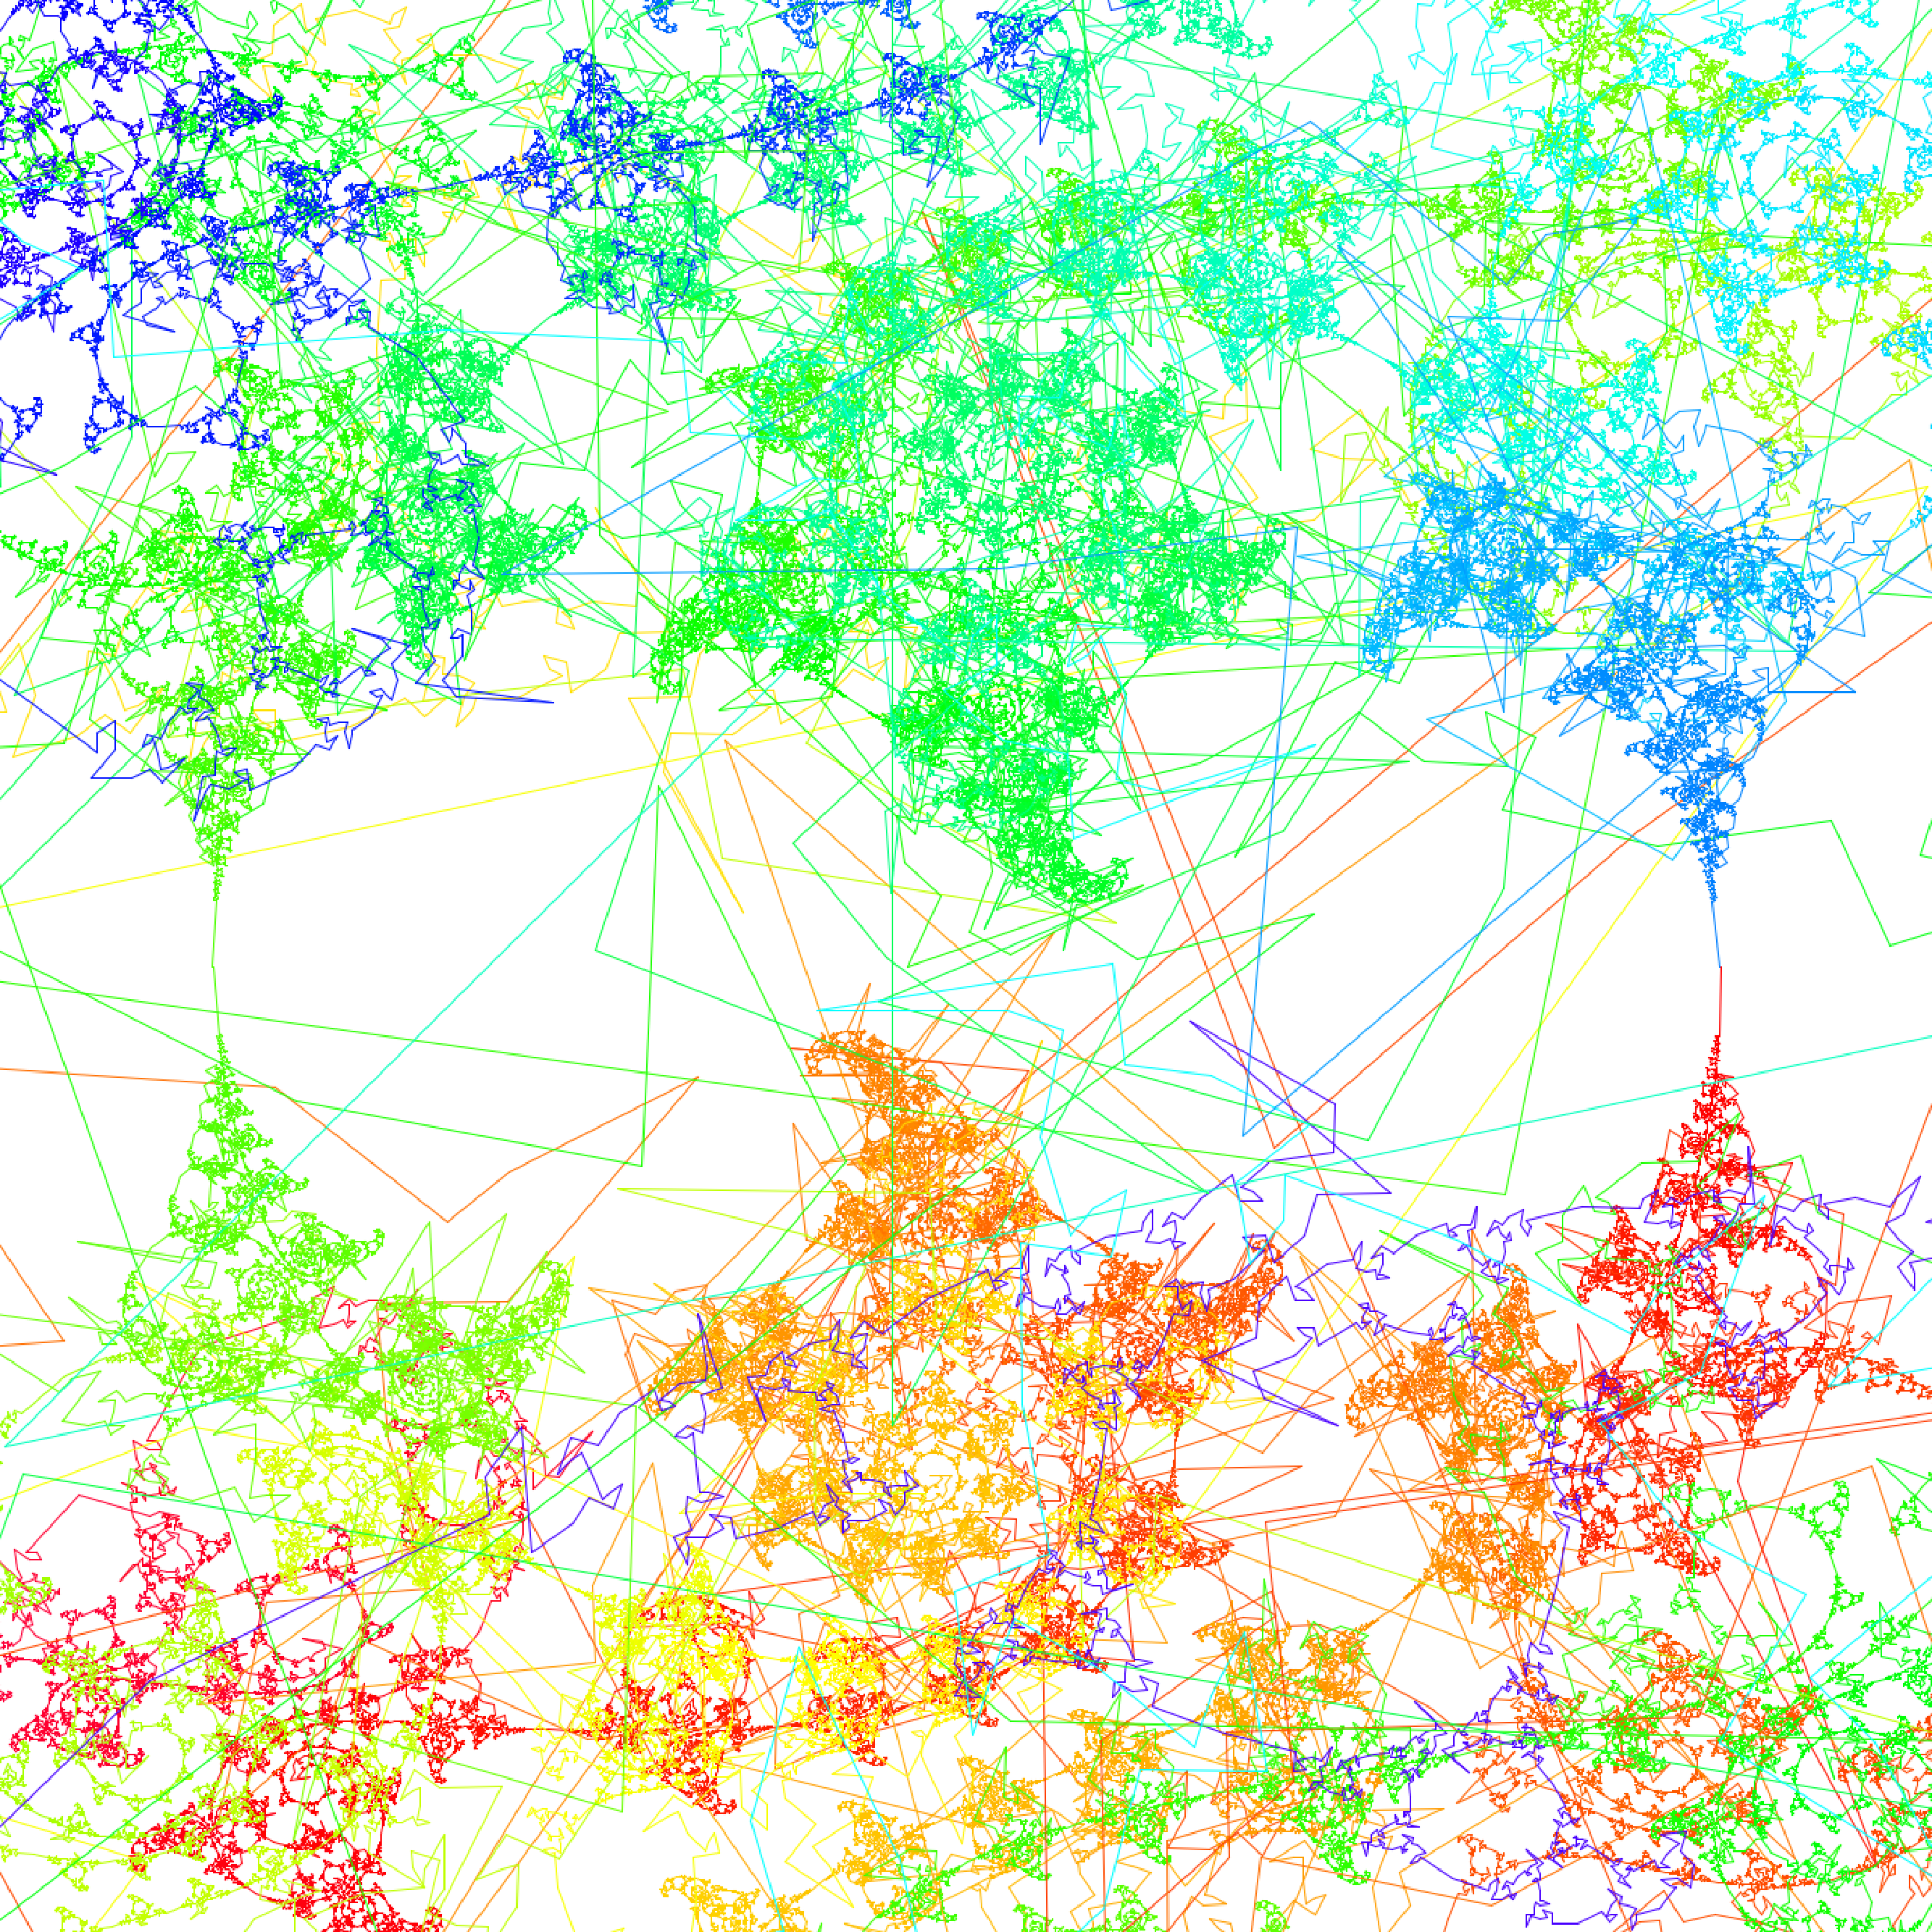
\includegraphics[ height=2.5in, keepaspectratio]{../img/klein/limitset/non-discrete2.pdf}
  \subcaption{}
 \end{minipage}
 \caption{The limit set of non-discrete groups}
\end{figure}

\subsubsection{Faults of Graph Traversal Approach}

グラフを探索する方法にはいくつかの欠点がある.
まず, 生成元や,探索を深くするごとに指数オーダーで計算量が増えてしまう.
また, 部分的に拡大したい場合に無駄な部分を計算しないといった処理にも手間
がかかる.
さらに木構造の探索は並列化に向かないため, 高速化が難しい.
そのため, 木構造の探索に頼らない方法がいくつか考案されている.

しかしながら, 最近のOpenCLやCUDAといった並列計算プラットフォームでは
Dynamic Parallelismという機能を用いることで,木構造探索の並列計算を行う
ことが可能である.
ただし, 最新のハードウェアに依存した機能のため, どの計算機環境でも使えるわけではない.

\subsection{Iterated Inversion System}

筆者らは, 1章でみたシェーダを用いたフラクタルのレンダリングアルゴリズム
に着想を得て, 円や球の反転で構成される群の軌道を高速に描画するためのアル
ゴリズム, \textit{Iterated Inversion System (IIS)}\cite{iis}を開発した.
円や球の座標と半径を直接計算するこれまでのアプローチに対して,このアルゴ
リズムは任意の点が属する円や球の深さを特定する.
これはスクリーンスペースのピクセルそれぞれに対して独立に計算することがで
きるので,シェーダによる並列計算,描画を行うことができる.

アルゴリズム自体は非常にシンプルである.
先にみた4つの反転円による群を考える.
このとき,黒い領域を基本領域とよぶ.
ある点がいずれかの反転円に属している時にその反転円に関する反転を行なうという操作を
反転後の点がすべての円の外側である基本領域に移されるまで繰り返す.
最終的に, 行なった反転の回数が, その点が属している円盤の深さとなる.
図\ref{fig:iis-orb}では青い点の軌道を描いている.
この点は二回反転が行なわれているので, 下から二番目の円に属している.
実際にこのアルゴリズムを用いてすべての点を基本領域へと移動させるためには,
無限回の反転が必要である. そのため, あらかじめ最大の反転回数を決めておく.
それぞれの計算はピクセルごとに行なうことができるため, 最大の反転回数と,円の数の
多項式時間で描画することができる.

このアルゴリズムをより一般化した擬似コードをアルゴリズム\ref{iis2d}に示す.
後に我々は単純な円の反転以外の生成元を導入する.
そこで,基本領域にある点に対しては恒等写像で, その他の点に対しては反転の合成を
適用する写像$G$を考え,これを反転の代わりに用いることとする.

 \begin{algorithm}
  \caption{Iterated Inversion System (IIS)}
  \label{iis2d}
  \begin{algorithmic}
   \REQUIRE count $= 0$ and coordinates $=$ position determined by
   pixel
   \FOR{$i=0$ to MAX\_INVERSION}
   \STATE inFundamentalDomain $\leftarrow$ \TRUE
   \FOR{ each map $G$ in Maps }
   \IF{$G$ is available to coordinates}
   \STATE coordinates $\leftarrow$ $G(\text{coordinates})$
   \STATE INCREMENT count
   \STATE inFundamentalDomain $\leftarrow$ \FALSE
   \ENDIF
   \ENDFOR
   \IF {inFundamentalDomain}
   \STATE BREAK for
   \ENDIF
   \ENDFOR
   \STATE RETURN count
  \end{algorithmic}
 \end{algorithm}

\begin{figure}[htbp]
 \center
 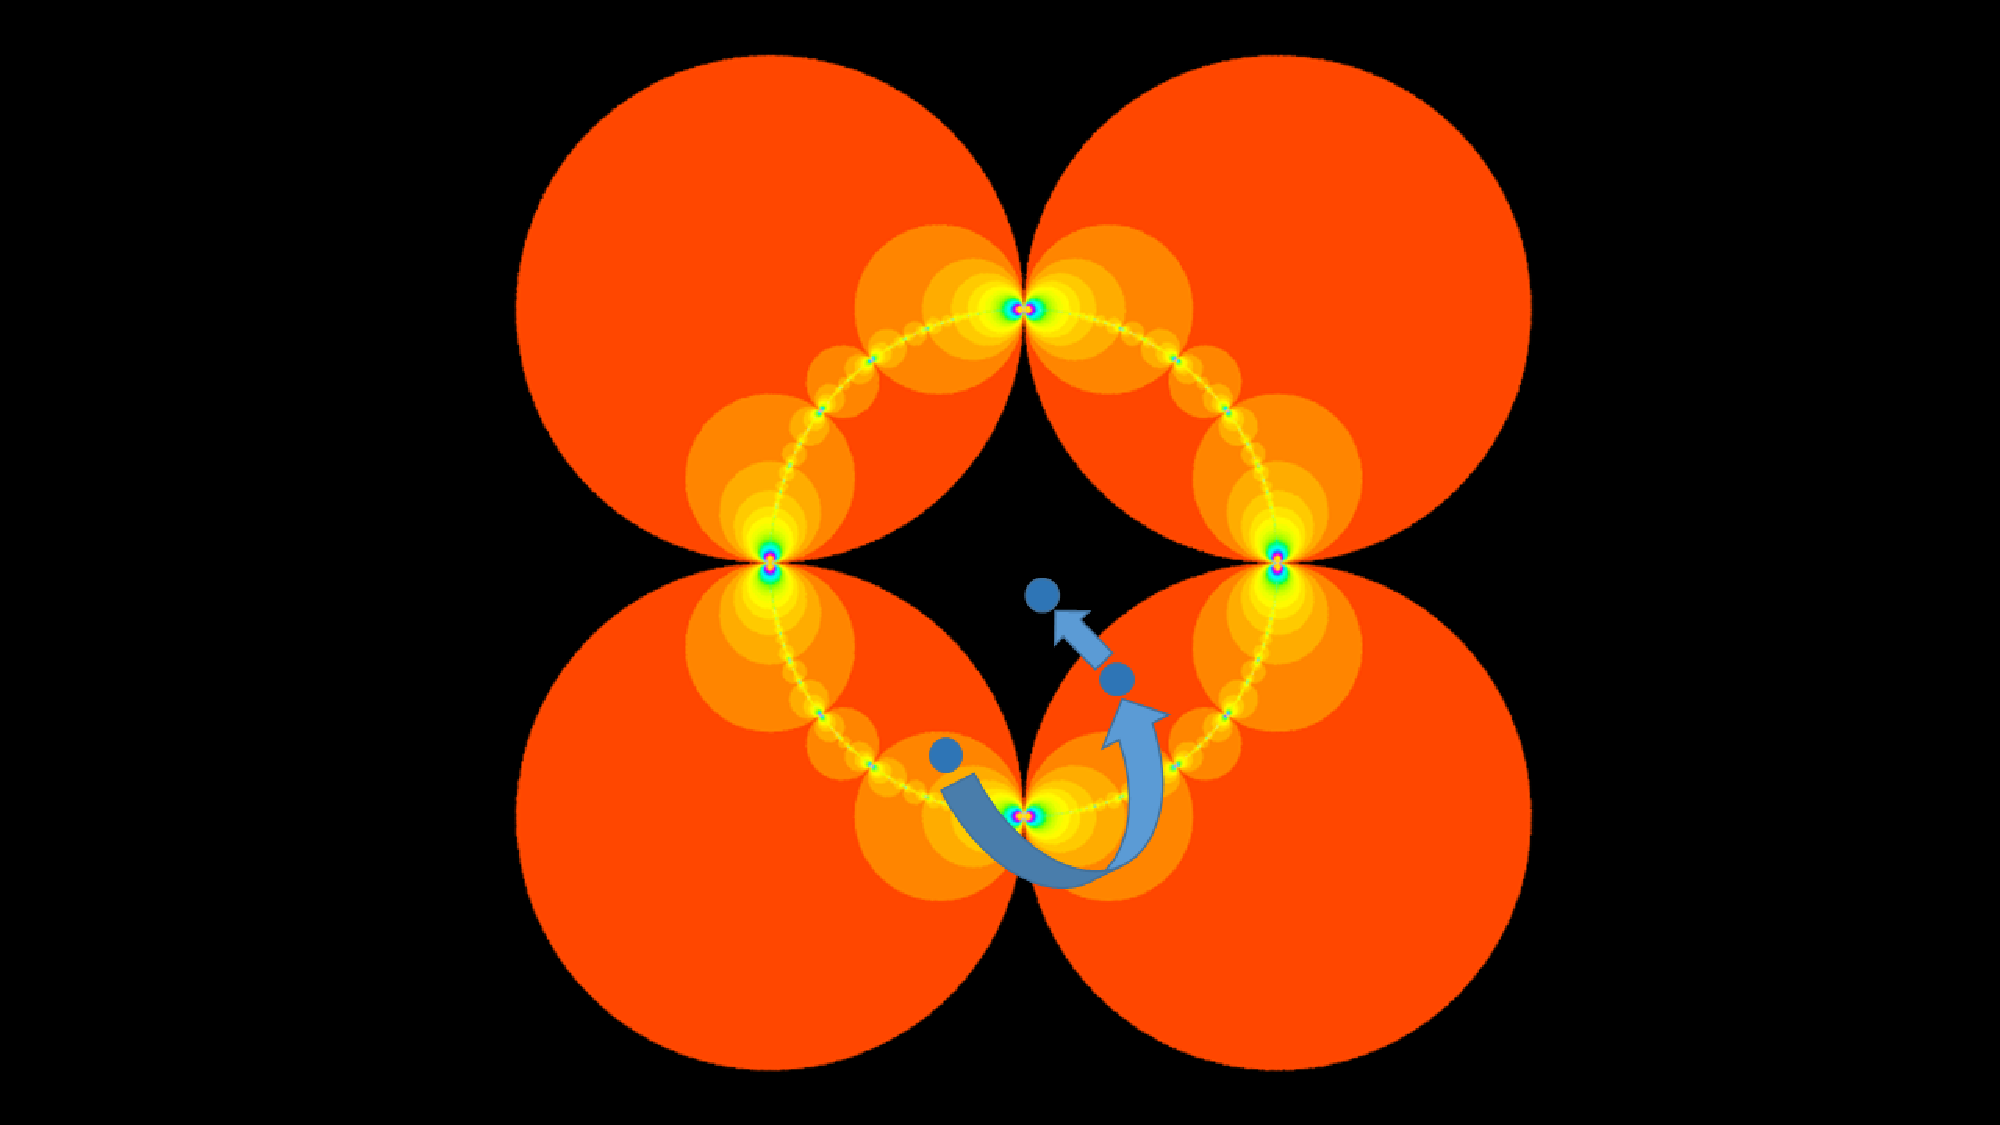
\includegraphics[ height=1.5in, keepaspectratio]{../img/klein/orb.pdf}
 \caption{Orbit}
 \label{fig:iis-orb}
\end{figure}

このアルゴリズムは三次元空間における球の反転に対しても用いることができる.
しかし,反転球の軌道は球の内側に入り込むため,二次元の場合と同様に描画するには手間がかかる.
そこで我々は軌道の元となる球を用意し, その球を反転球の反転の組み合わせで移した軌道を描画する.
これはレイマーチングとDistance Estimationを用いることで高速に描画することができる.

図\ref{fig:simpleGen3d}における灰色の球を\emph{反転球},緑色の球を\emph{基本球}とよぶ.
基本球をすべての反転球の反転の組合わせで移すと図\ref{fig:simpleOrb3d}のよう
な形状が得られる.
基本球の数を増やすことも可能である. 図\ref{fig:3baseSphere}は3つの基本球
の軌道を描画した.

レイマーチングに用いる距離関数を求めるため,
ここで簡単のために, 図\ref{fig:iis-orb}のXY平面での断面を考えることにする.
これを図\ref{fig:xySlice}に示した.
橙色の円列はショットキー球の軌道, 水色の円が基本球の軌道である.
緑色の点$P2$をレイの先端であるとすると最も近い球は$S2$となる.
しかし, $S2$の位置と半径は分からない.
そこで我々は変換のヤコビアンを用いて, 基本球である$S1$の位置と半径から距離を逆算する.

反転球の中心を$S$その半径を$R$,半径を適用する前の点を$P$とおくと
球の反転のヤコビアンは以下のように計算できる.
$ Jacobian = R^2 / distance(P, S)^2 $
また, 半径が無限大の球の反転のヤコビアンは1であることに注意する.

距離関数では,レイの先端にIISを作用させ,
球の反転のヤコビアンを反転をおこなう毎にかけあわせていく.
最終的に基本領域上の点と基本球との距離をヤコビアンの積で割ることで近似された距離を求めることができる.

この近似は荒いため, もう一つ考慮すべき事がある.
レイの先端が極限集合より外側にあるとき, その点は球の反転によって外側に移さ
れるため, 距離関数が正しく機能せず,大きな距離を返してしまい,
レイは予期せずしてオブジェクトを突きぬけてしまう.
よってオブジェクトの前面が正しくレンダリングされずに,
図\ref{fig:artifact}のような乱れを生みだす.

このような不具合を避けるため, 算出された距離を縮小する方法をとった.
距離の縮小率は球の大きさによって実験的に決められる.

基本球の大きさを変更することで, 形状を変形することができる.
図\ref{fig:limitSetOnSphere}は基本球の大きさを極限集合と同じ大きさにしたものである.
球の上に極限集合が描画されていることがわかる.

一般化した擬似コードはアルゴリズム\ref{iis3d}に示した.

\begin{figure}[htbp]
 \begin{minipage}[b]{0.5\hsize}
  \begin{minipage}[]{0.49\hsize}
   \center
   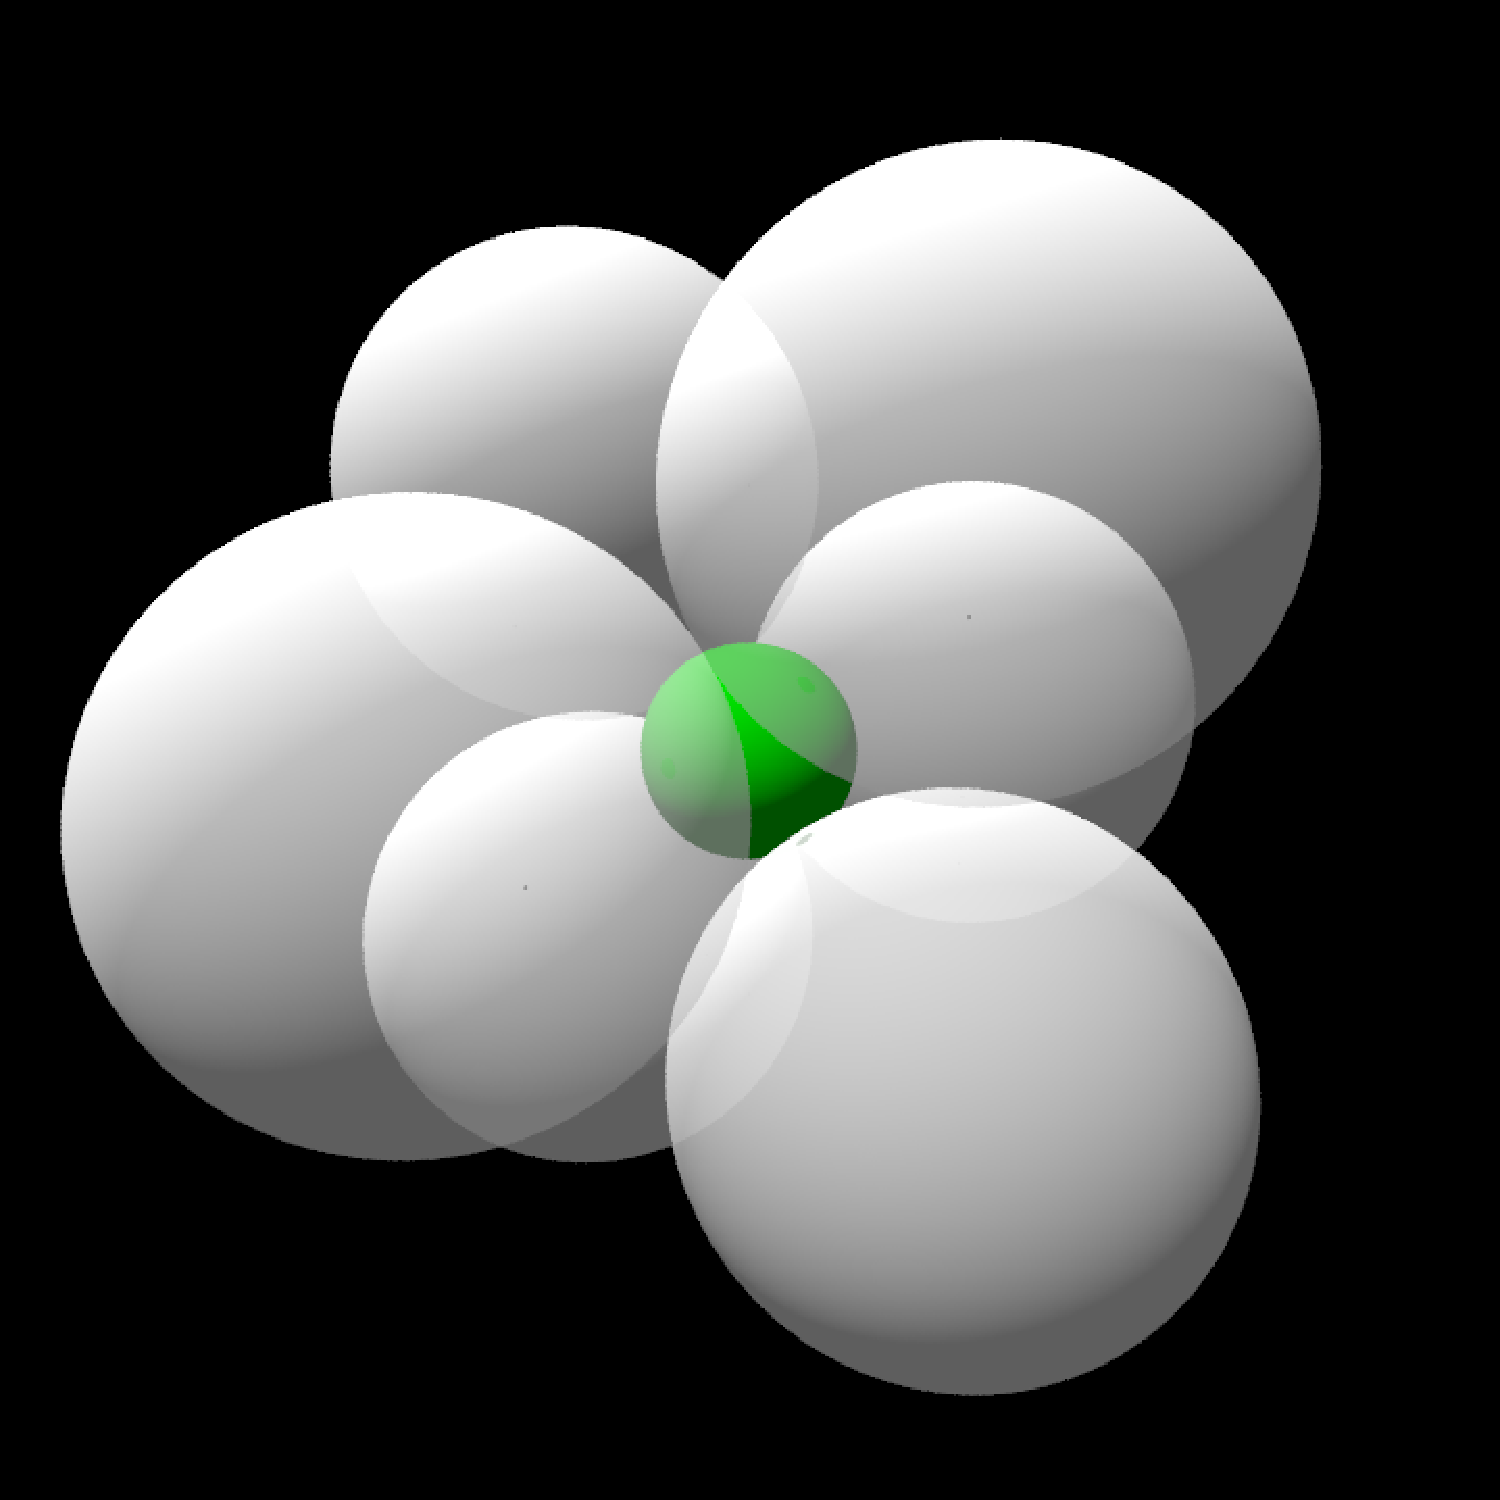
\includegraphics[ height=1.5in, keepaspectratio]{../img/klein/simpleGen.pdf}
   \subcaption{Generator}
   \label{fig:simpleGen3d}
  \end{minipage}
  \begin{minipage}[]{0.49\hsize}
   \center
   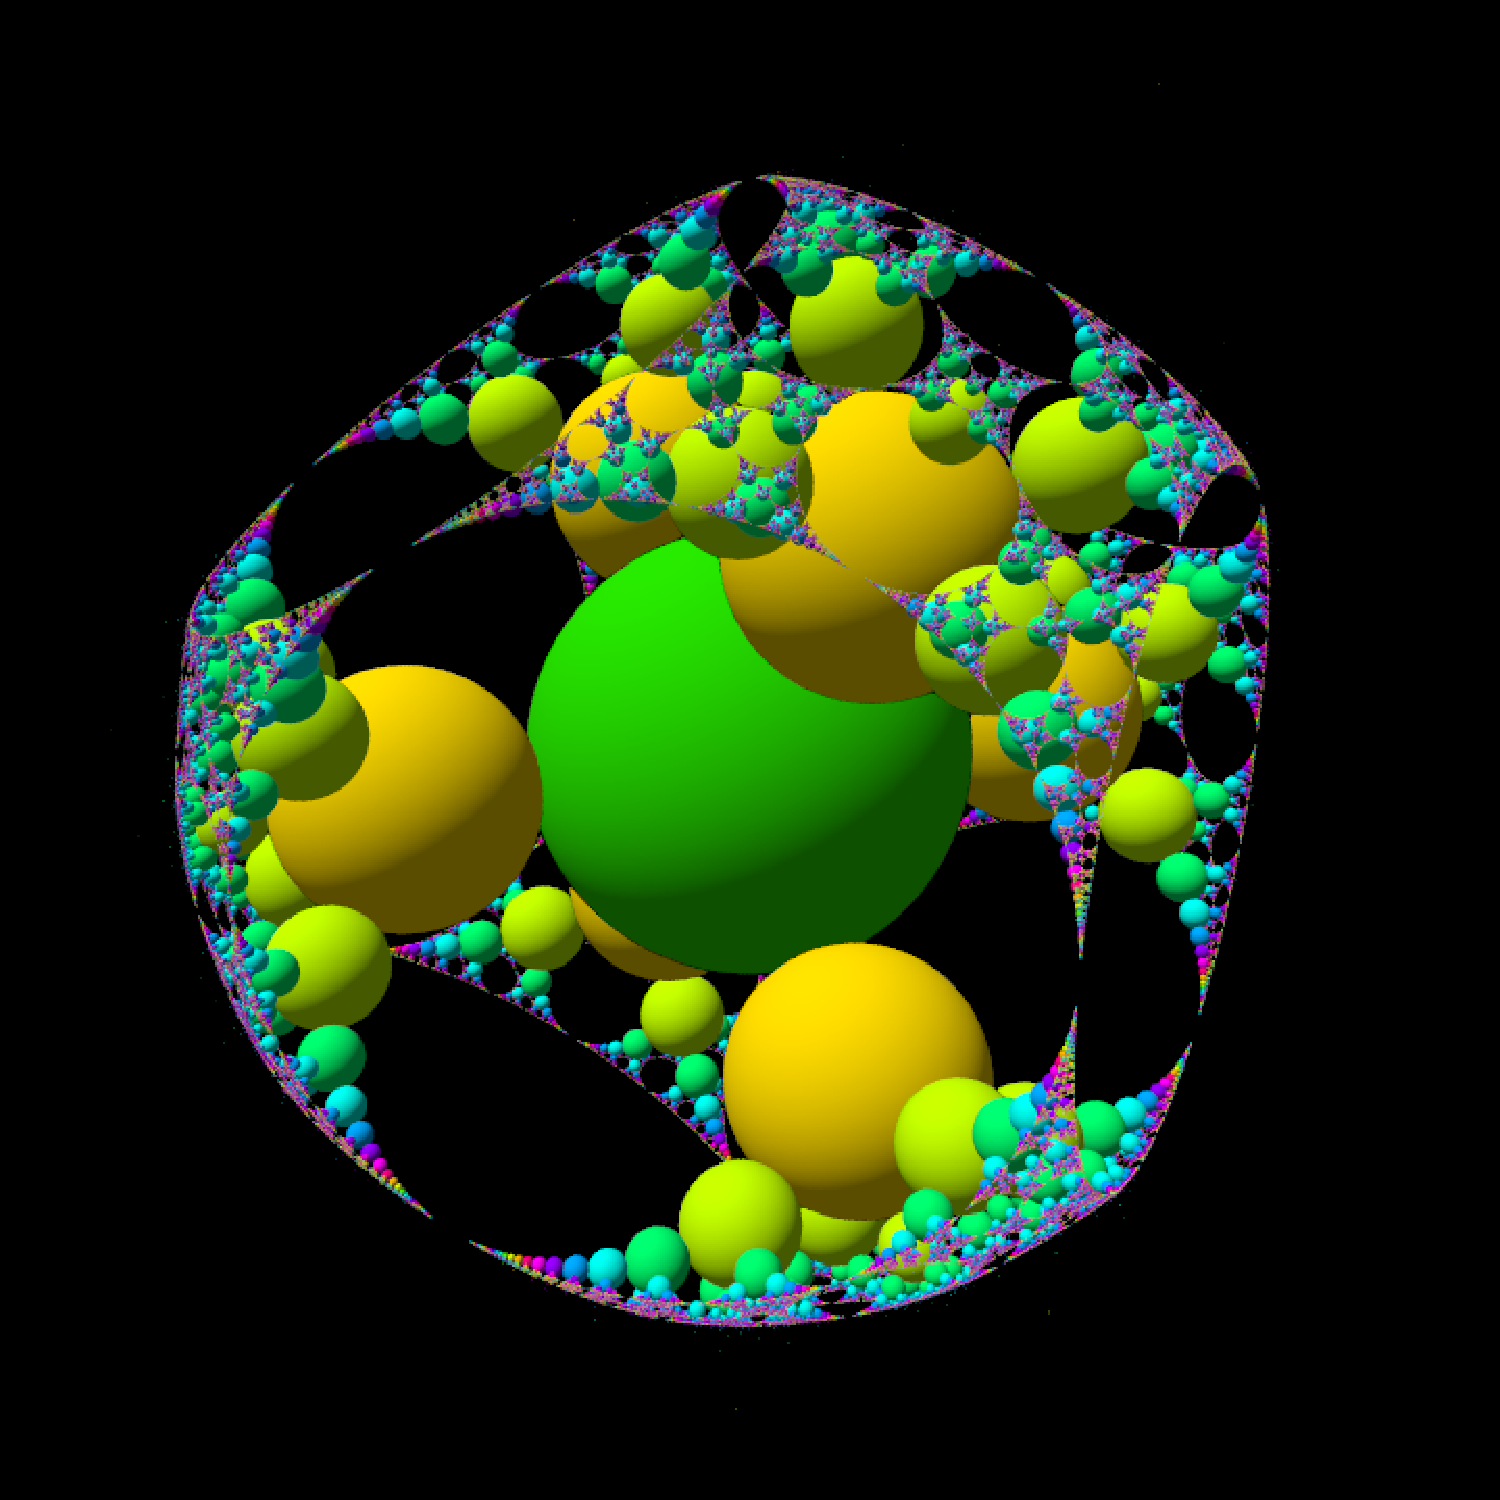
\includegraphics[ height=1.5in, keepaspectratio]{../img/klein/simpleOrbit.pdf}
   \subcaption{Orbit}
   \label{fig:simpleOrb3d}
  \end{minipage}
  \caption{The orbit of the green sphere}
  \label{fig:iis-orb}
 \end{minipage}
 \begin{minipage}[b]{0.5\hsize}
  \center
  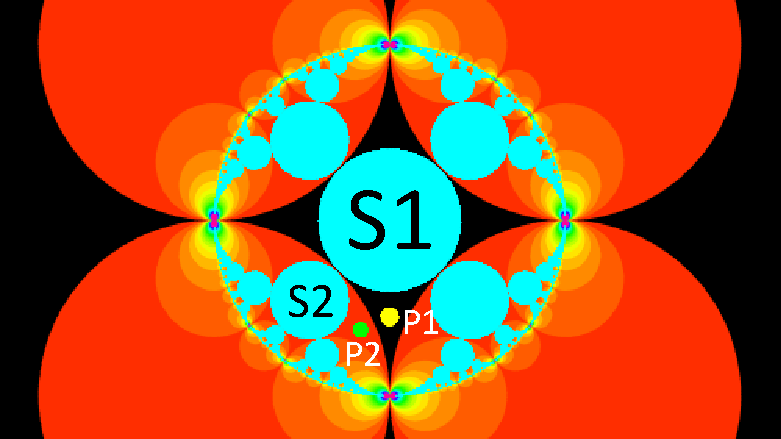
\includegraphics[ height=1.5in, keepaspectratio]{../img/klein/xySlice.pdf}
  \caption{XY-slice image of Figure \ref{fig:iis-orb}}
  \label{fig:xySlice}
 \end{minipage}
\end{figure}

\begin{figure}[htbp]
 \begin{minipage}{0.5\hsize}
  \center
  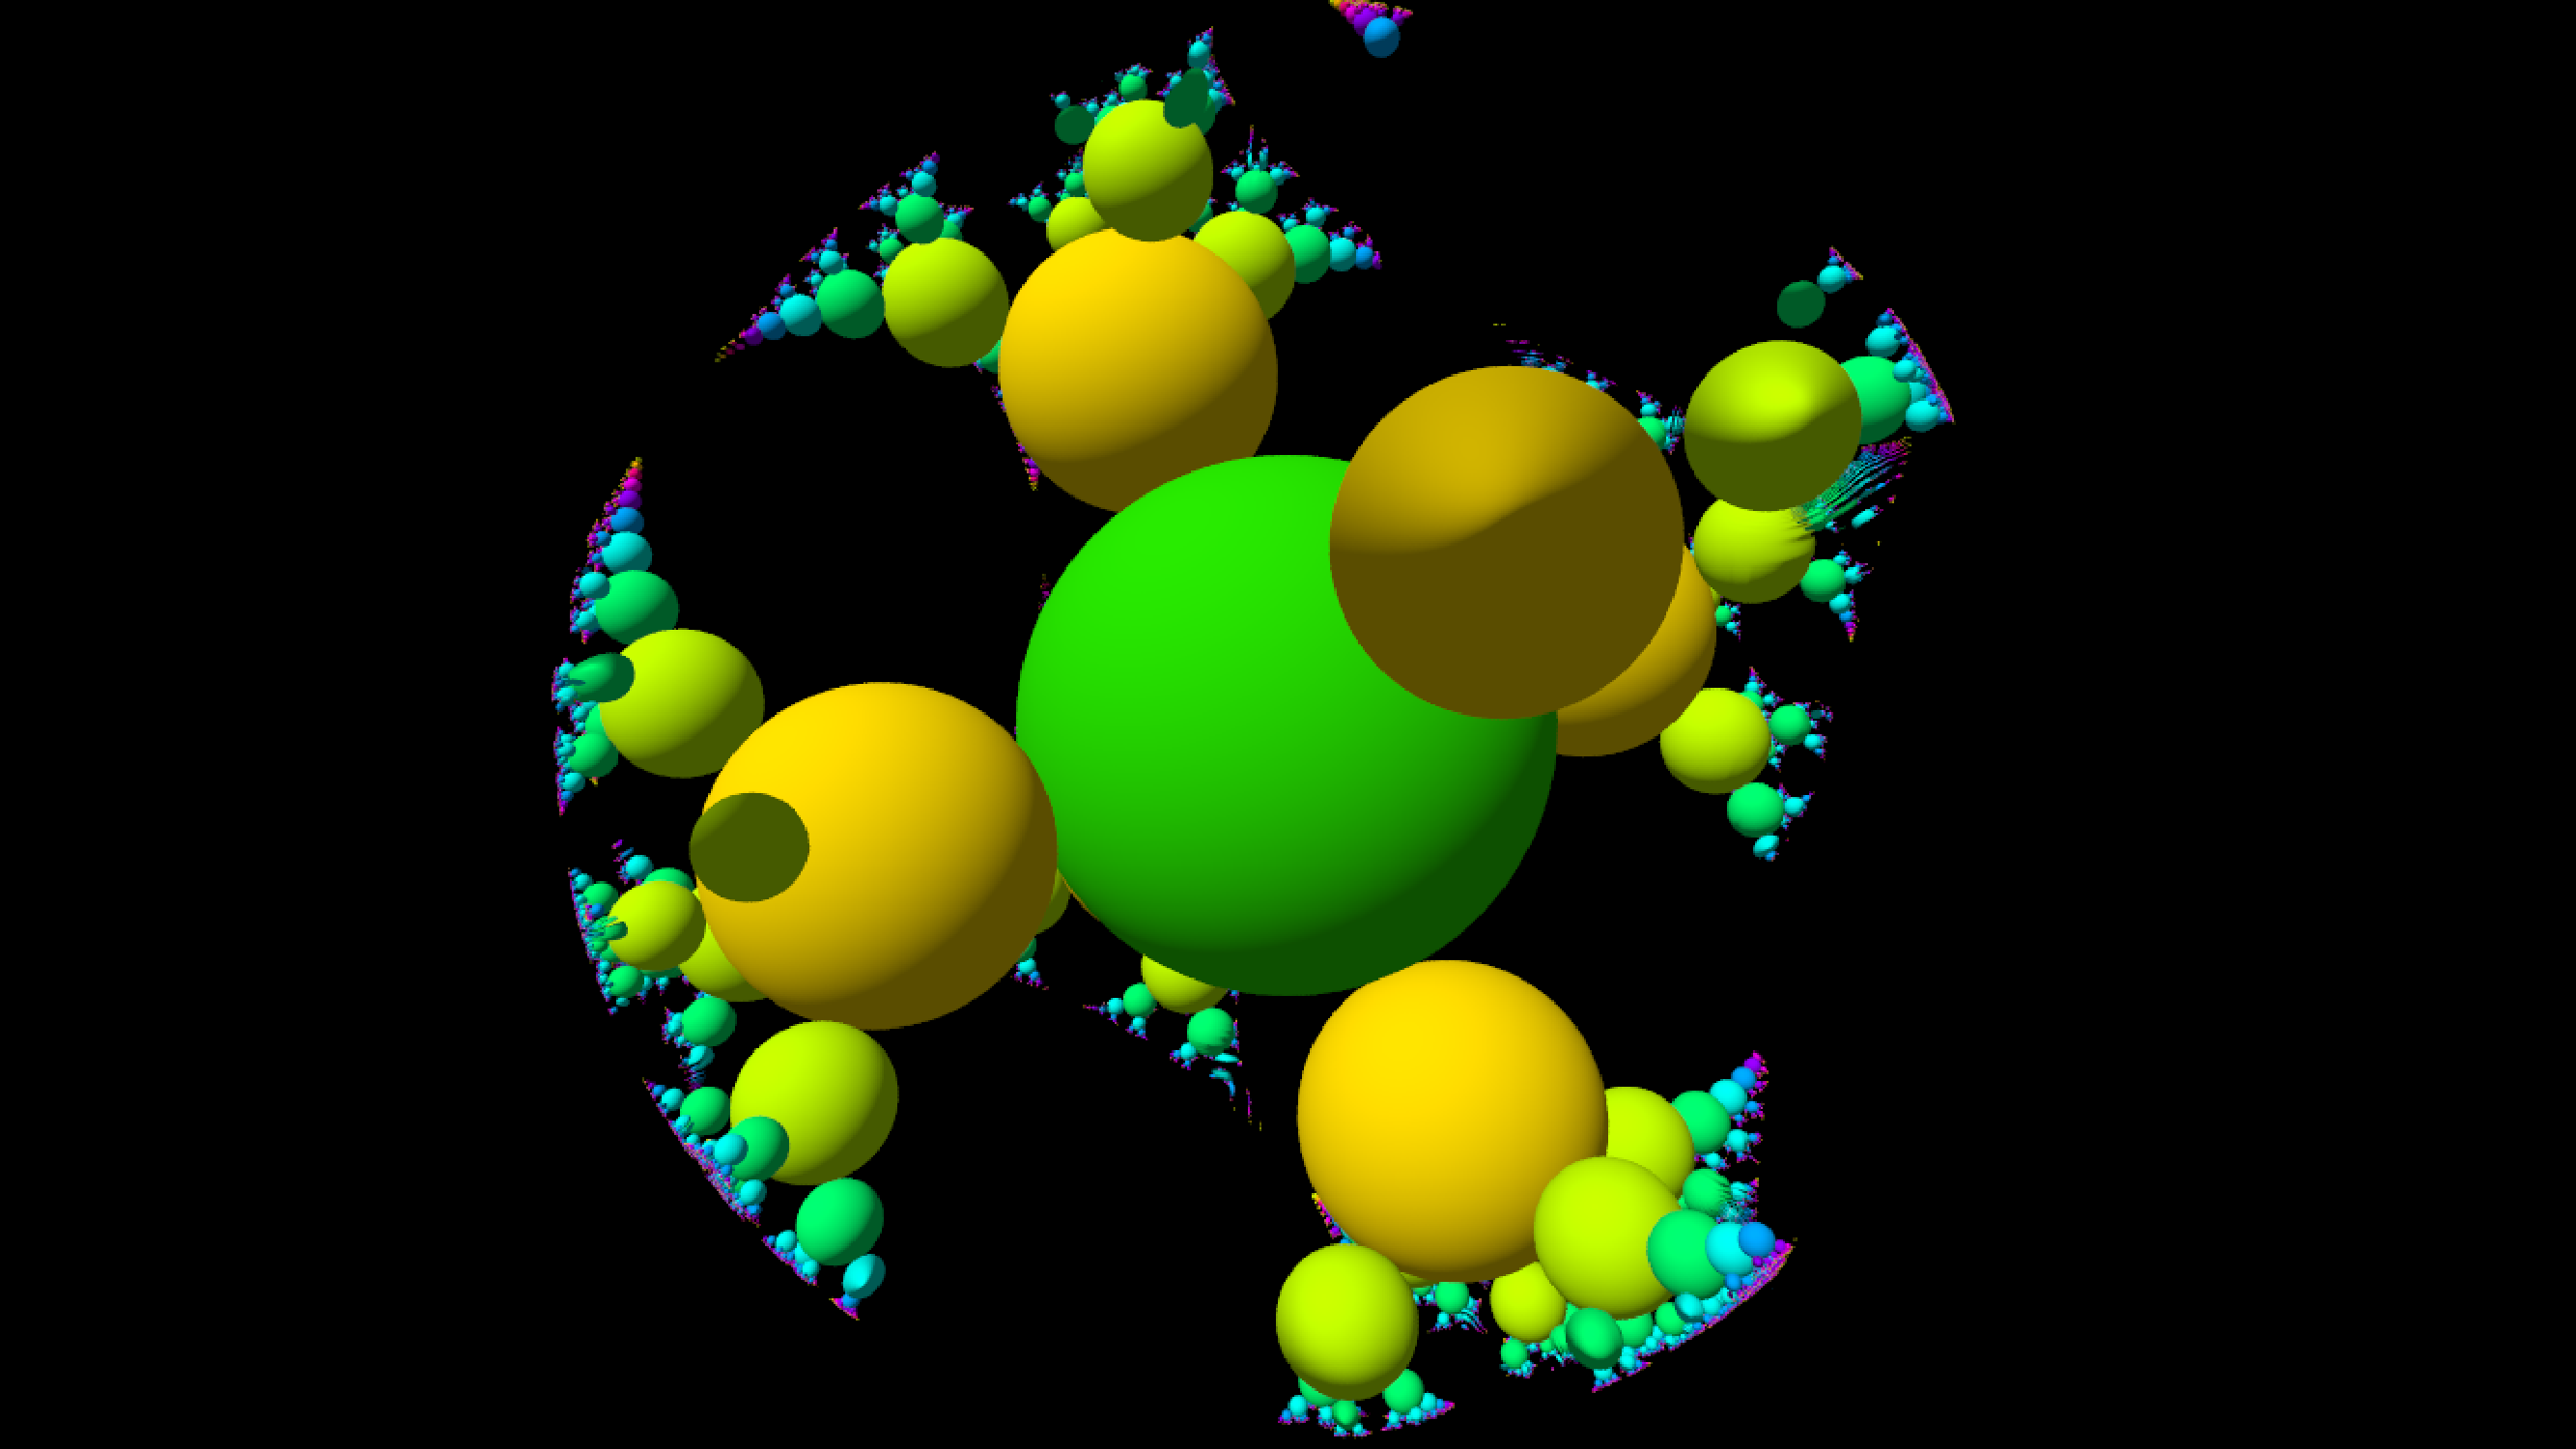
\includegraphics[ height=1.5in, keepaspectratio]{../img/klein/artifact.pdf}
  \caption{The Artifact}
  \label{fig:artifact}
 \end{minipage}
 \begin{minipage}{0.5\hsize}
  \center
  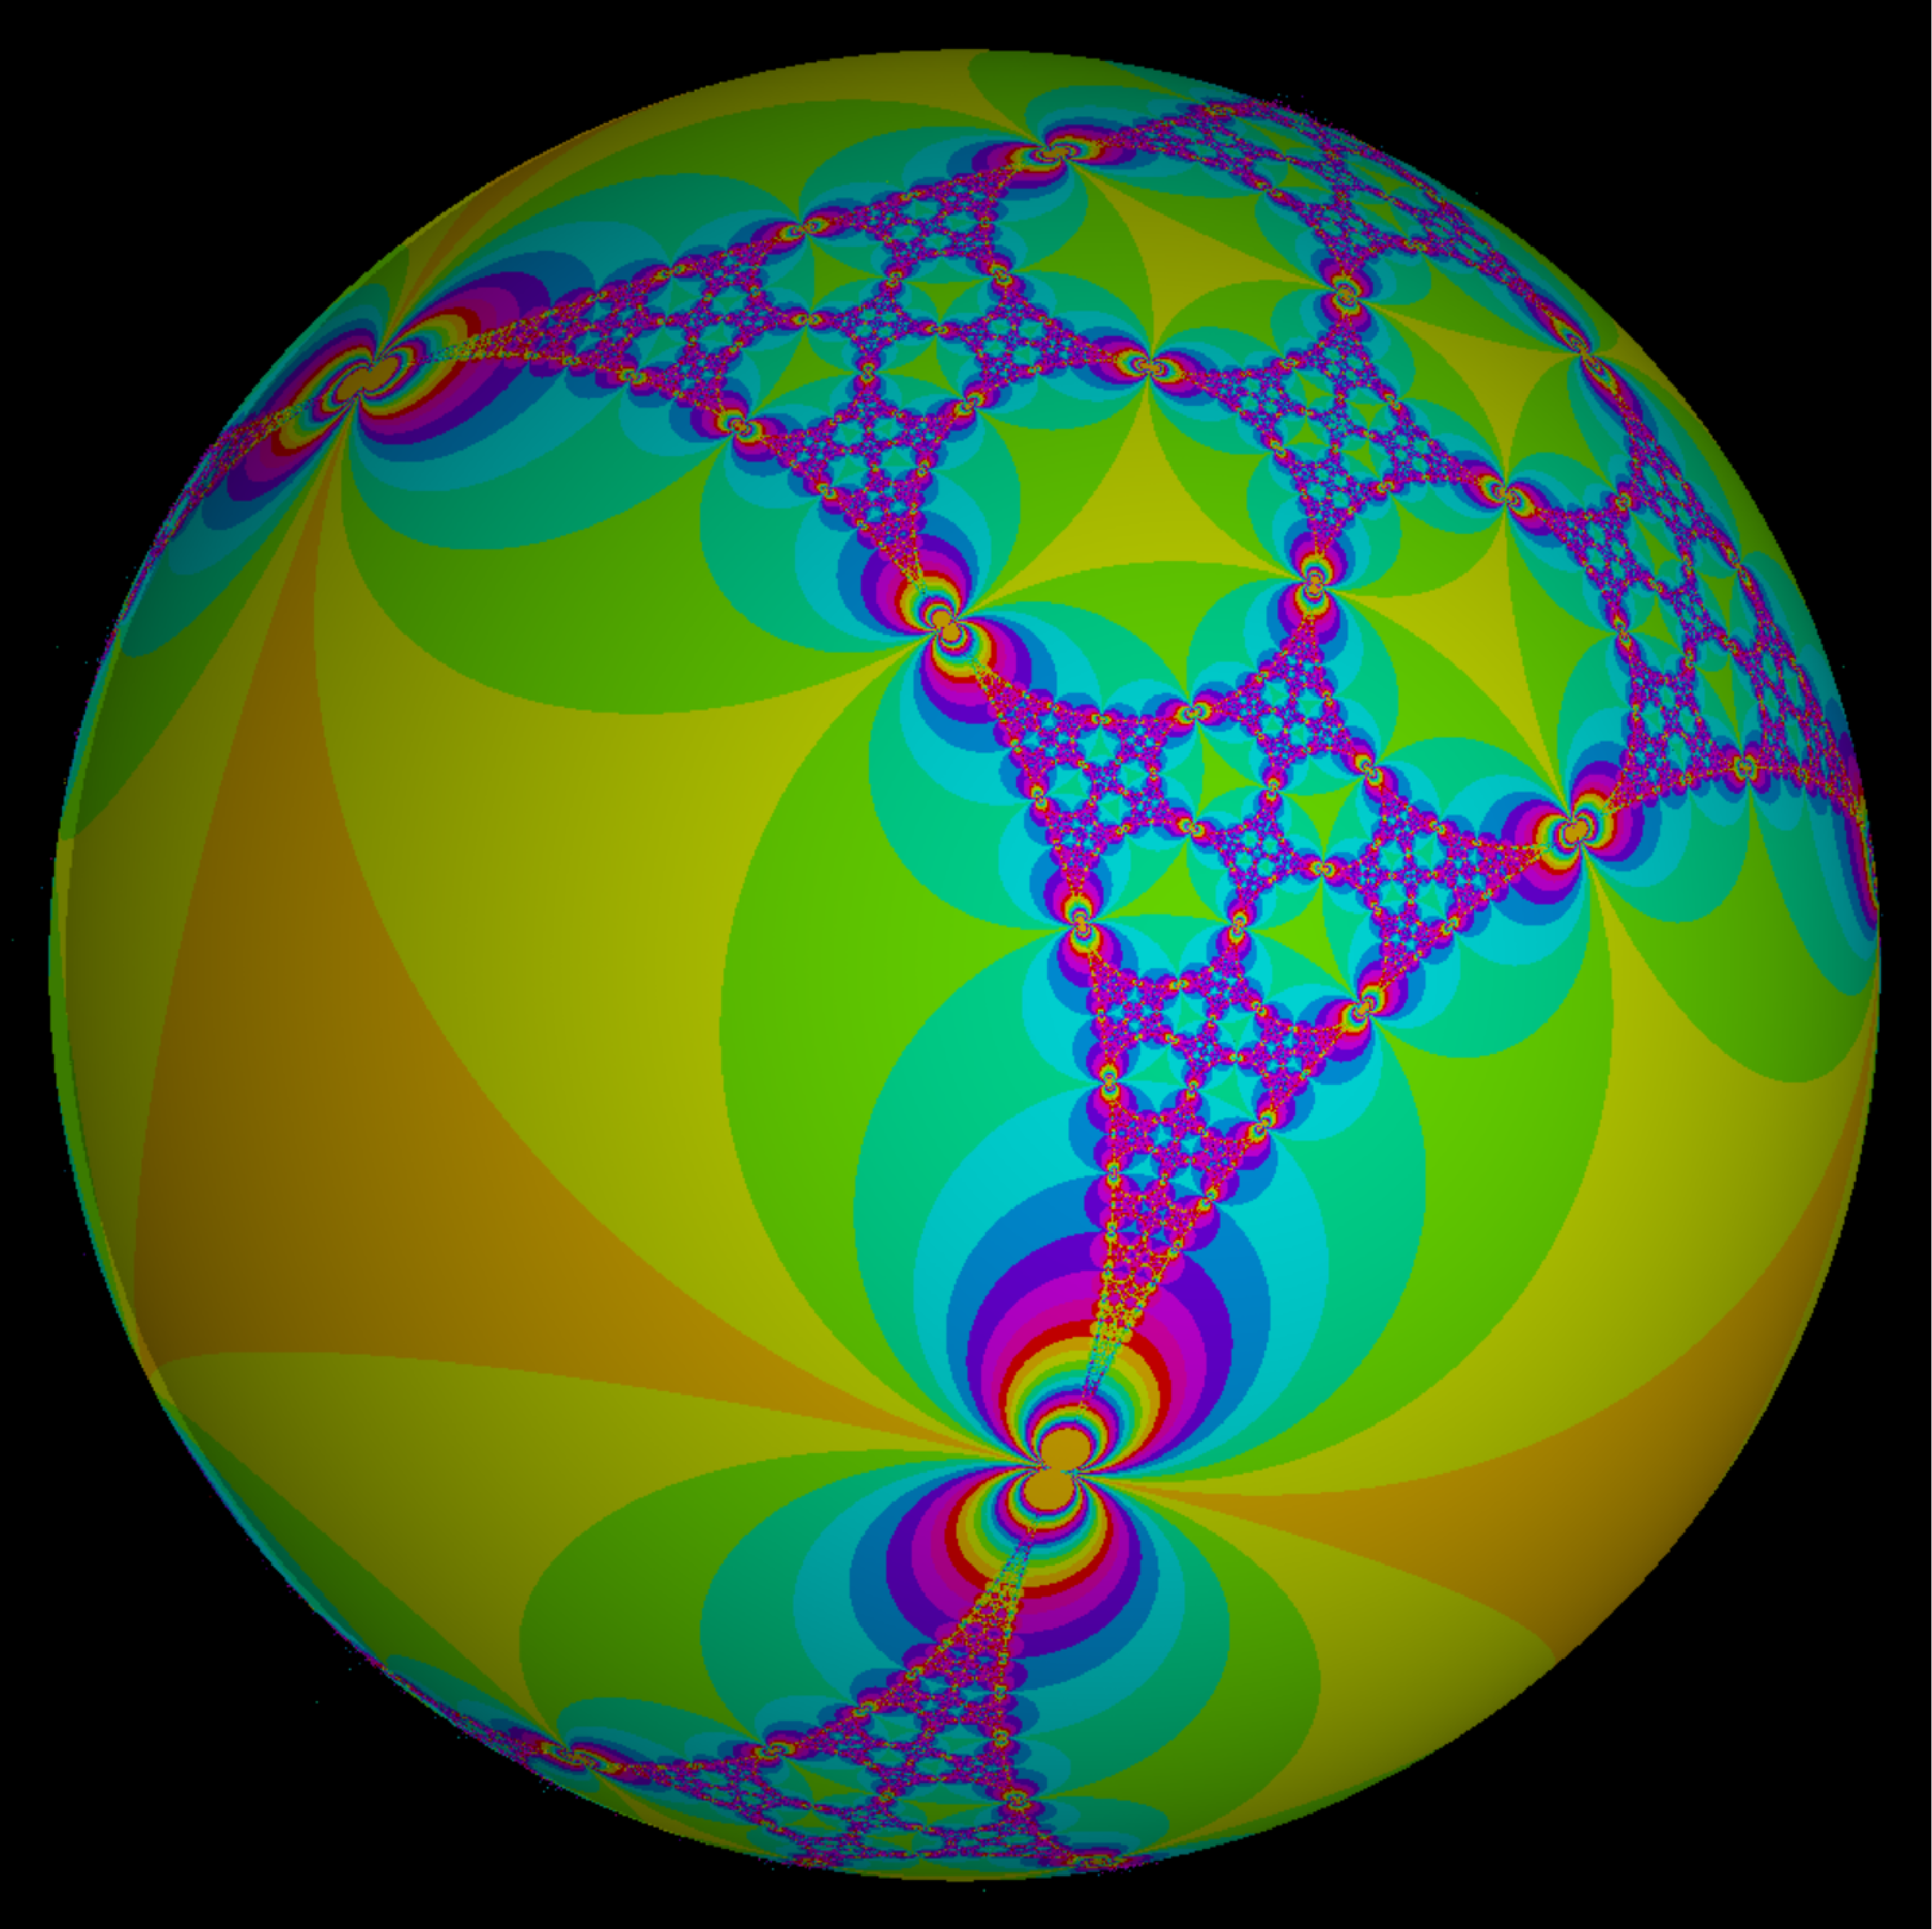
\includegraphics[ height=1.5in, keepaspectratio]{../img/klein/3dLimitSet.pdf}
  \caption{The Limit set on the sphere}
  \label{fig:limitSetOnSphere}
 \end{minipage}
\end{figure}

\begin{figure}[htbp]
 \begin{minipage}{0.5\hsize}
  \center
  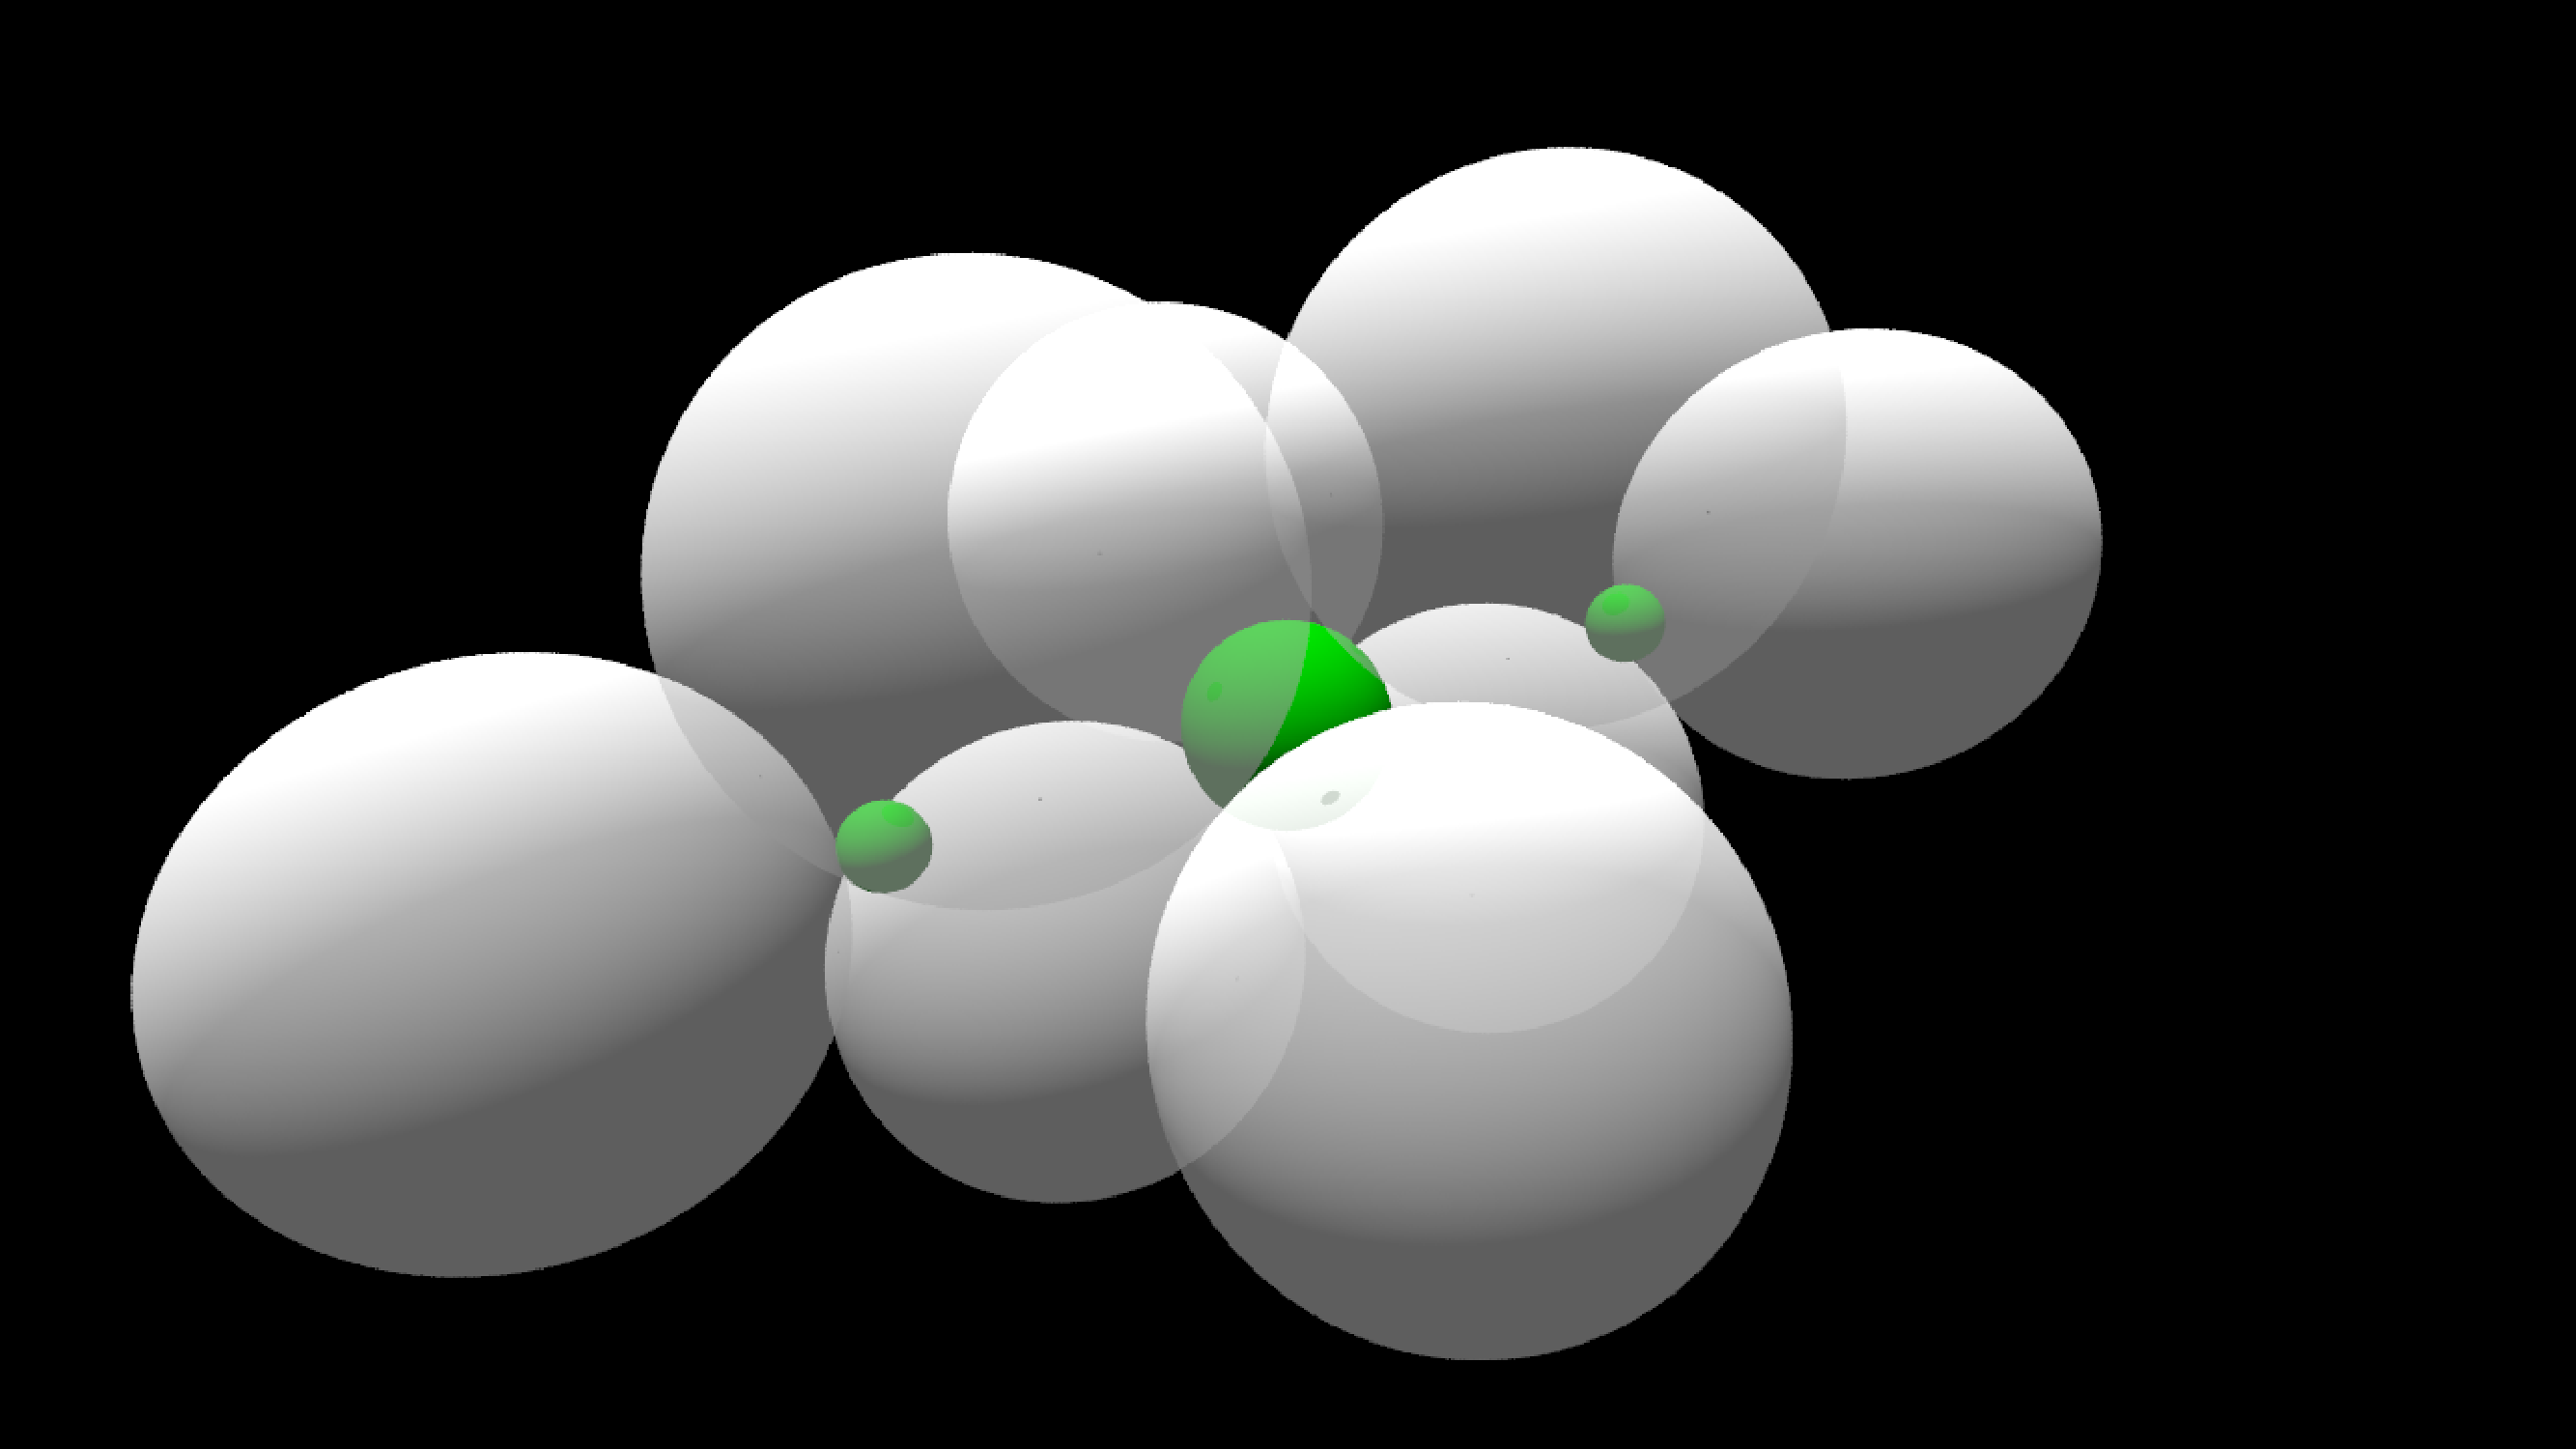
\includegraphics[ height=1.5in, keepaspectratio]{../img/klein/3baseGen.pdf}
  \subcaption{Generator}
  \label{fig:}
 \end{minipage}
 \begin{minipage}{0.5\hsize}
  \center
  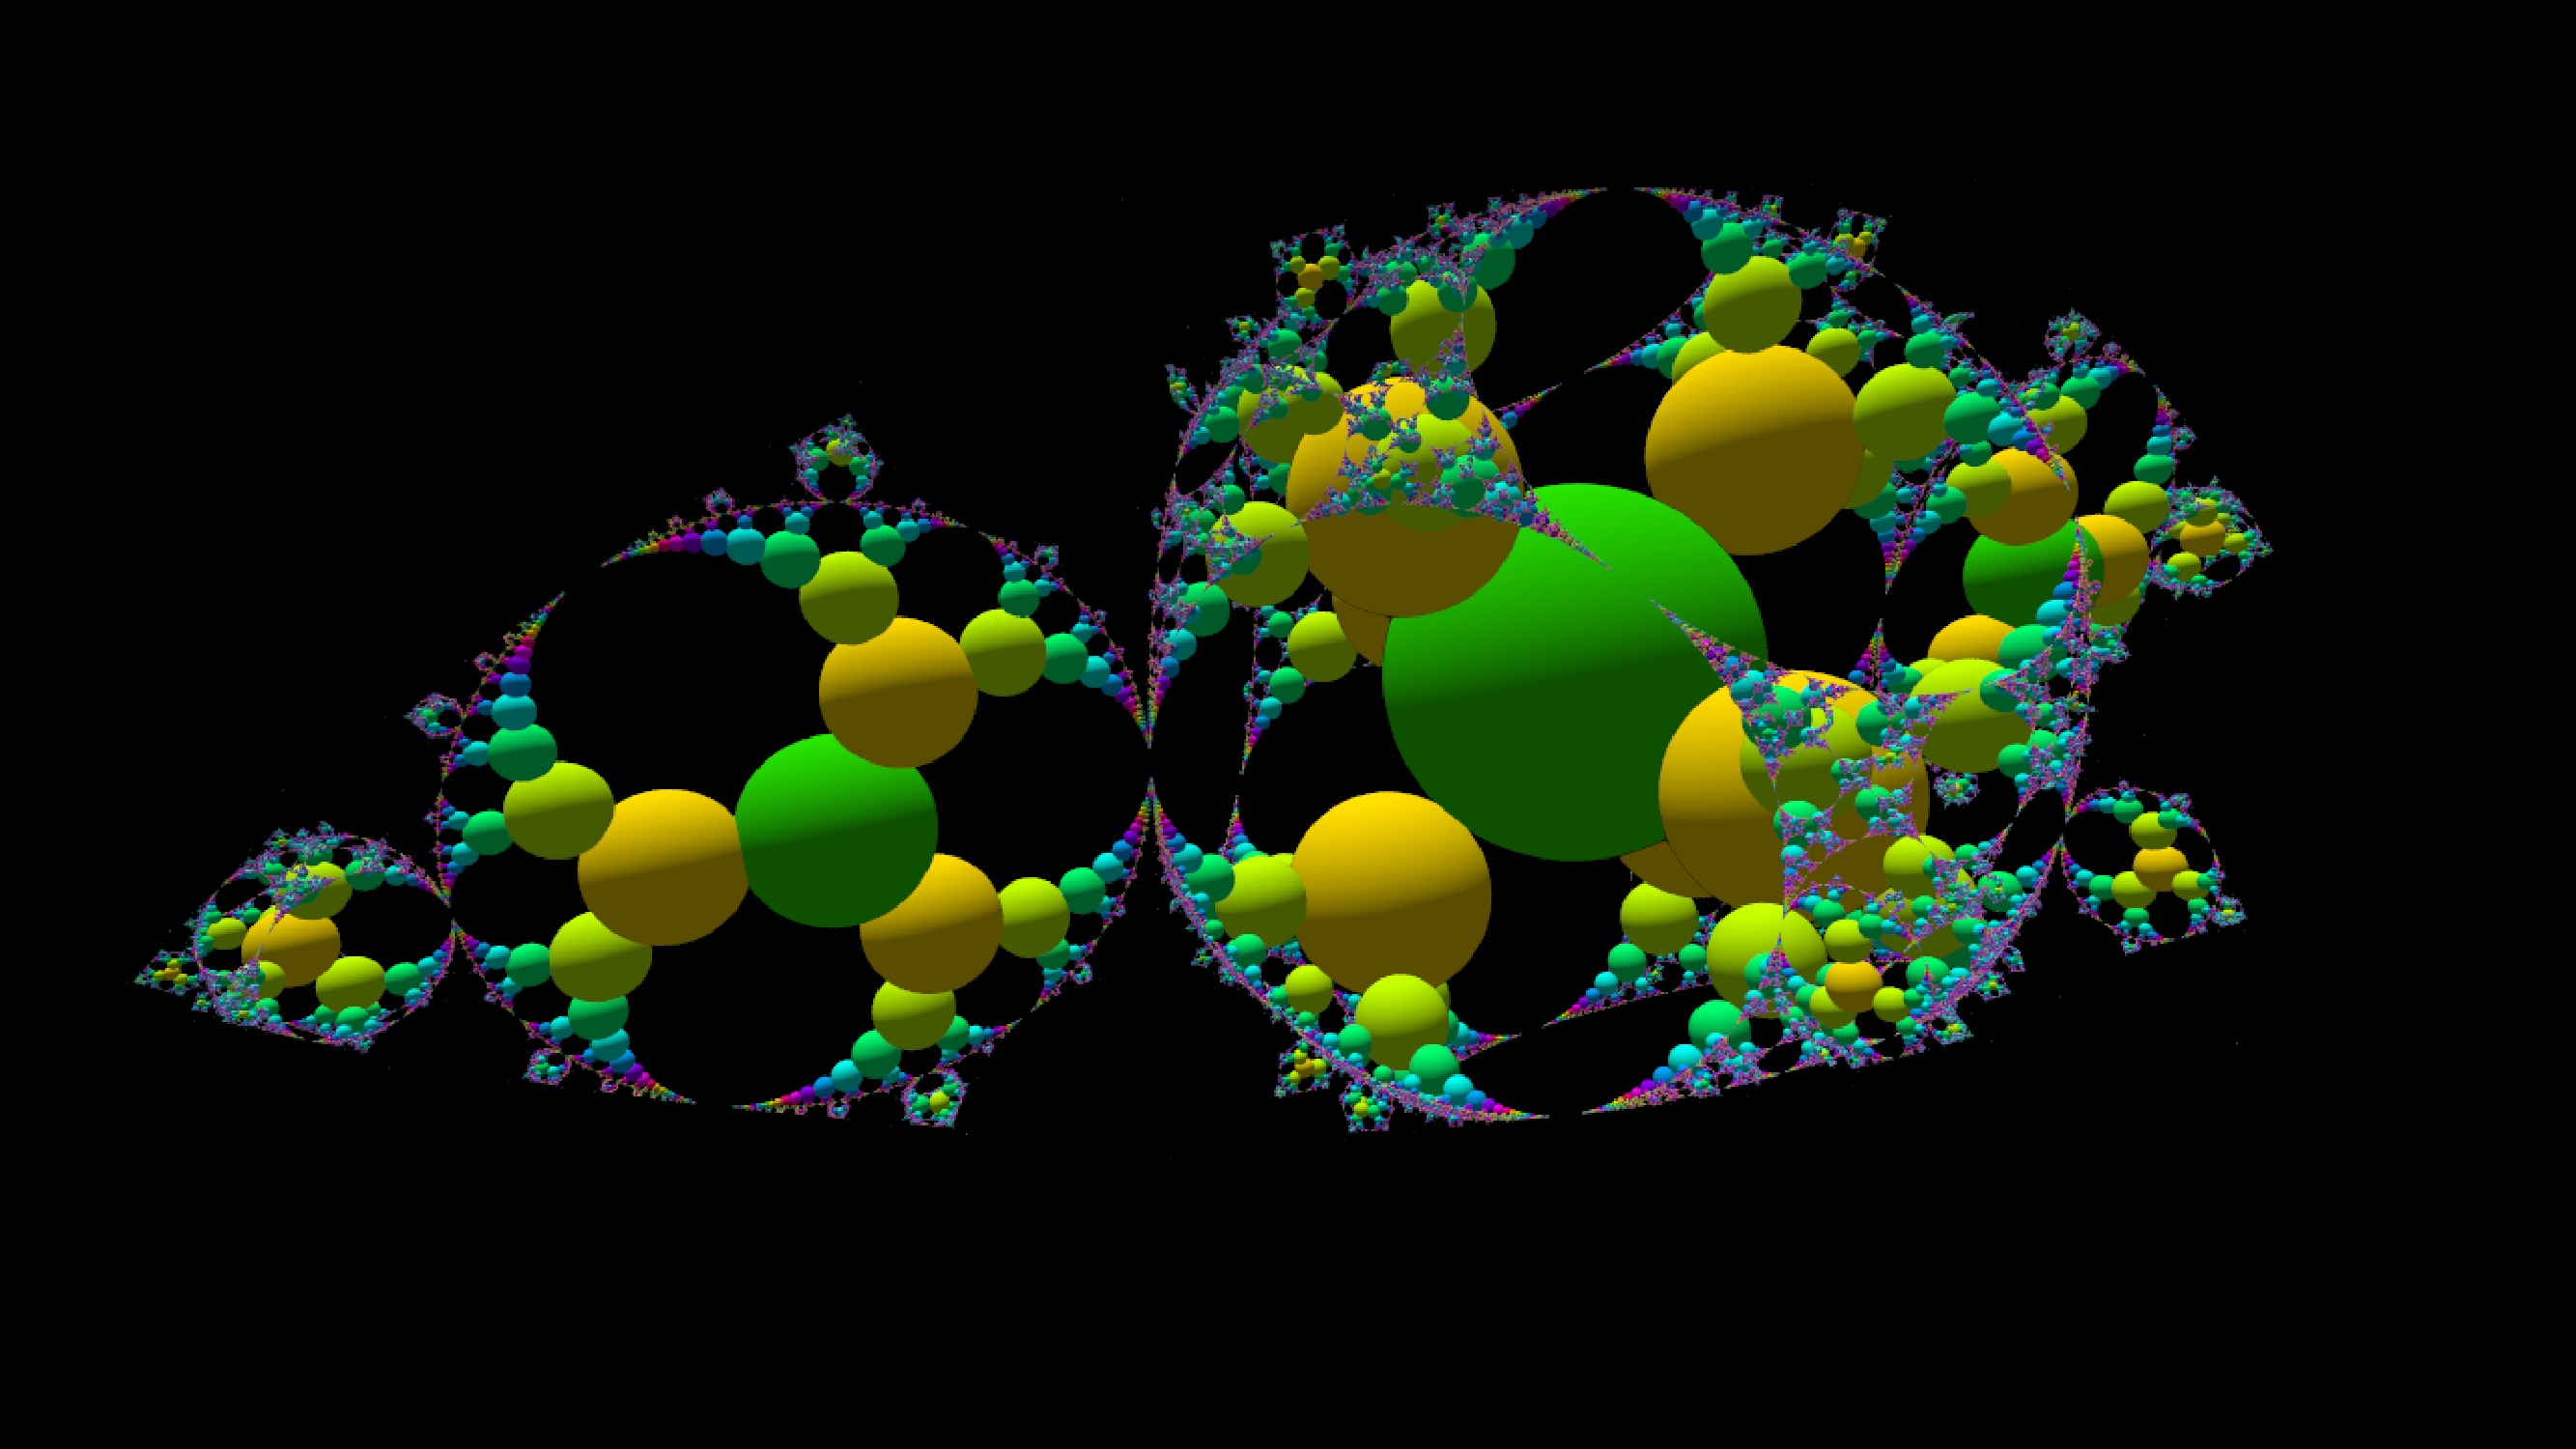
\includegraphics[ height=1.5in, keepaspectratio]{../img/klein/3baseOrb.pdf}
  \subcaption{Orbit}
  \label{fig:}
 \end{minipage}
 \caption{The orbit of 3 base spheres}
 \label{fig:3baseSphere}
\end{figure}

\begin{algorithm}
 \caption{Distance function}
 \label{iis3d}
 \begin{algorithmic}
  \REQUIRE count $= 0$, $d$ = MAX\_DISTANCE, $dr = 1.0$, and coordinates $=$ tipping
  point of the ray
  \FOR{$i=0$ to MAX\_INVERSION}
  \STATE inFundamentalDomain $\leftarrow$ \TRUE
  \FOR{ each Map $G$ in Maps}
  \IF{$G$ is available to coordinates}
  \STATE coordinates $\leftarrow$ $G(\text{coordinates})$
  \STATE $dr \leftarrow dr * $ (Jacobian of $G(\text{coordinates})$)
  \STATE INCREMENT count
  \STATE inFundamentalDomain $\leftarrow$ \FALSE
  \ENDIF
  \ENDFOR
  \IF {isInFundamentalDomain}
  \STATE BREAK for
  \ENDIF
  \ENDFOR
  \FOR{ each BaseSphere $S$ in BaseSpheres}
  \STATE $d \leftarrow$ min($d$, scalingFactor * (distance(coordinates, $S$.center) $-$
  $S$.radius) $/$ (absolute value of $dr$))
  \ENDFOR
  \RETURN $d$
 \end{algorithmic}
\end{algorithm}

\subsection{Geometrical Representation of M\"obius Transformations}

木構造を用いて群を可視化する際には,変換を行列で考えたが,行列表現でメビ
ウス変換を操作することは直観が得にくい.
例えば,行列による変換の表現から変換の作用を推測することは非常に難しい.

また,三次元空間に作用するメビウス変換を考えることで,高次元のクライン群を作ることができる.
図は四次元クライン群の極限集合を可視化したものである.
このように,三次元上での捩じれをもつ非常に興味深い形状が得られる.
しかし,このような群を構成するメビウス変換は,
四元数行列で表現されるため,さらに複雑な代数計算が必要となる.

そこで筆者はすべてのメビウス変換を円や球の反転で構成し,その軌道を描くことを考えた.
円や球を用いることで,幾何学的な直観が働き,生成元と可視化される図形の間の関係性を
容易に理解することができる.
それに加え,IISを用いることで複雑な生成元をもつ群もリアルタイムに可視化
することができる.
このことは,研究者や学習者だけでなく,フラクタルアーティストにも有益なも
のになる.
筆者は円や球の反転で構成される群をインタラクティブに構成するウェブアプリケーション,
{\it Schottky Link} \footnote{Schottky Link:
\url{https://schottky.jp}}を開発している.

\subsubsection{2D Generators}

\noindent\textbf{Simple Inversion}
先に述べたように, 円に関する反転は複素平面の向きを変えるので, メビウス変
換ではない.
ふたつの反転円がペアとなってはじめてメビウス変換となる.
しかし, ここでは簡単のためにメビウス変換の元として扱う.

\noindent\textbf{Inversion of a Circle with Infinite Radius}
無限の半径をもつ円に関する反転は直線に関する反転で表される.
図\ref{fig:infCircle}では右側の反転円が左側の半径無限の円の内側に反転で移されていることがわ
かる.

\noindent\textbf{Rotation}
二つの交差する直線の反転の組み合わせは回転を表わす. 回転角は二直線のなす
角の二倍である. 図\ref{fig:rotation}では90度回転を示した. また, 軌道となる円同士がお互いに
重なりあわないようにするためには, 回転角は有理角である必要がある.

\noindent\textbf{Parallel Translation}
平行な二直線による反転の組は平行移動を表す.
図\ref{fig:translation2d}では二つの無限の半径をもつ円が向かい合っている.
これらの円の反転によって,中央の4つの反転円はx軸方向に移されている.
平行移動の固定点は無限遠点であり,これは放物型変換である.

\noindent\textbf{Composition of Two Circles}
二つの同心円をもちいることで, 双曲型変換である単純な拡縮を表わすことがで
きる.
図\ref{fig:scaling2d}における赤い円を$C1$,緑の円を$C2$, そして青い円を$C1'$とよぶ.
$C1'$は$C1$を$C2$による反転で移した像である.
図\ref{fig:scaling2d}では, 白い縁をもつ二つの円の軌道を描いている.
固定点は円の中心と無限遠点である.
写像$G$は以下のように定義される.
また,ここで接頭辞$I$は反転を表わす.
例えば, $I_{C1}$は$C1$による反転を表わす.
\begin{align*}
 G =
  \begin{cases}
   I_{C2} \circ I_{C1} & (\text{The point is inside of } C1) \\
   I_{C1} \circ I_{C2} & (\text{The point is outside of } C1')
  \end{cases}
\end{align*}
$G$を点に繰り返し作用させることで基本領域へと移動させることができる.
この種類の生成元の基本領域は青と緑の領域である.
完全な円の軌道をIISを用いて描くには, 反転円をこの領域内に配置す
る必要がある.

次に$C1$を少し動かすと, 図\ref{fig:hyperbolic2d}のような軌道が得られる.
無限遠点の固定点は有限の点に移り,有限の固定点は, $C1$の内部で移動する.
二つの円が交差しない限り, これも双曲型変換である.

$C1$と$C2$が接触する時, 図\ref{fig:parabolic2d}のように,固定点はその交点で重なりあい, 放物型変換となる.

\noindent\textbf{Loxodromic}
上記の生成元の軌道は実数による拡縮と共役であった.
この生成元にさらに二つの反転を加えることで軌道に捻りを加えることができる.
図\ref{fig:loxodromic2d}における$C1$と$C2$の中心を通る白い直線を$L$,
黄色の円を$C3$, そして水色の点を$P$とよぶ.
$P$は制御点であり, $C3$は$P$とその$C1$と$C2$による反転の像である$P'$と
$P''$の三点から定義される.
$L$と$C3$の反転の組み合わせは回転を表し,これが軌道に捻りを加える.

写像$G$は以下のようになる.
\begin{align*}
G =
\begin{cases}
 (I_{C2} \circ I_{C1}) \circ (I_{C3} \circ I_L) & (\text{The point is inside of } C1) \\
 (I_L \circ I_{C3}) \circ (I_{C1} \circ I_{C2}) & (\text{The point is outside of }C1')
\end{cases}
\end{align*}
また, 二つの固定点からこの種類の生成元を得ることもできる.

\begin{figure}[h!tbp]
 \begin{minipage}[t]{0.3\hsize}
  \center
   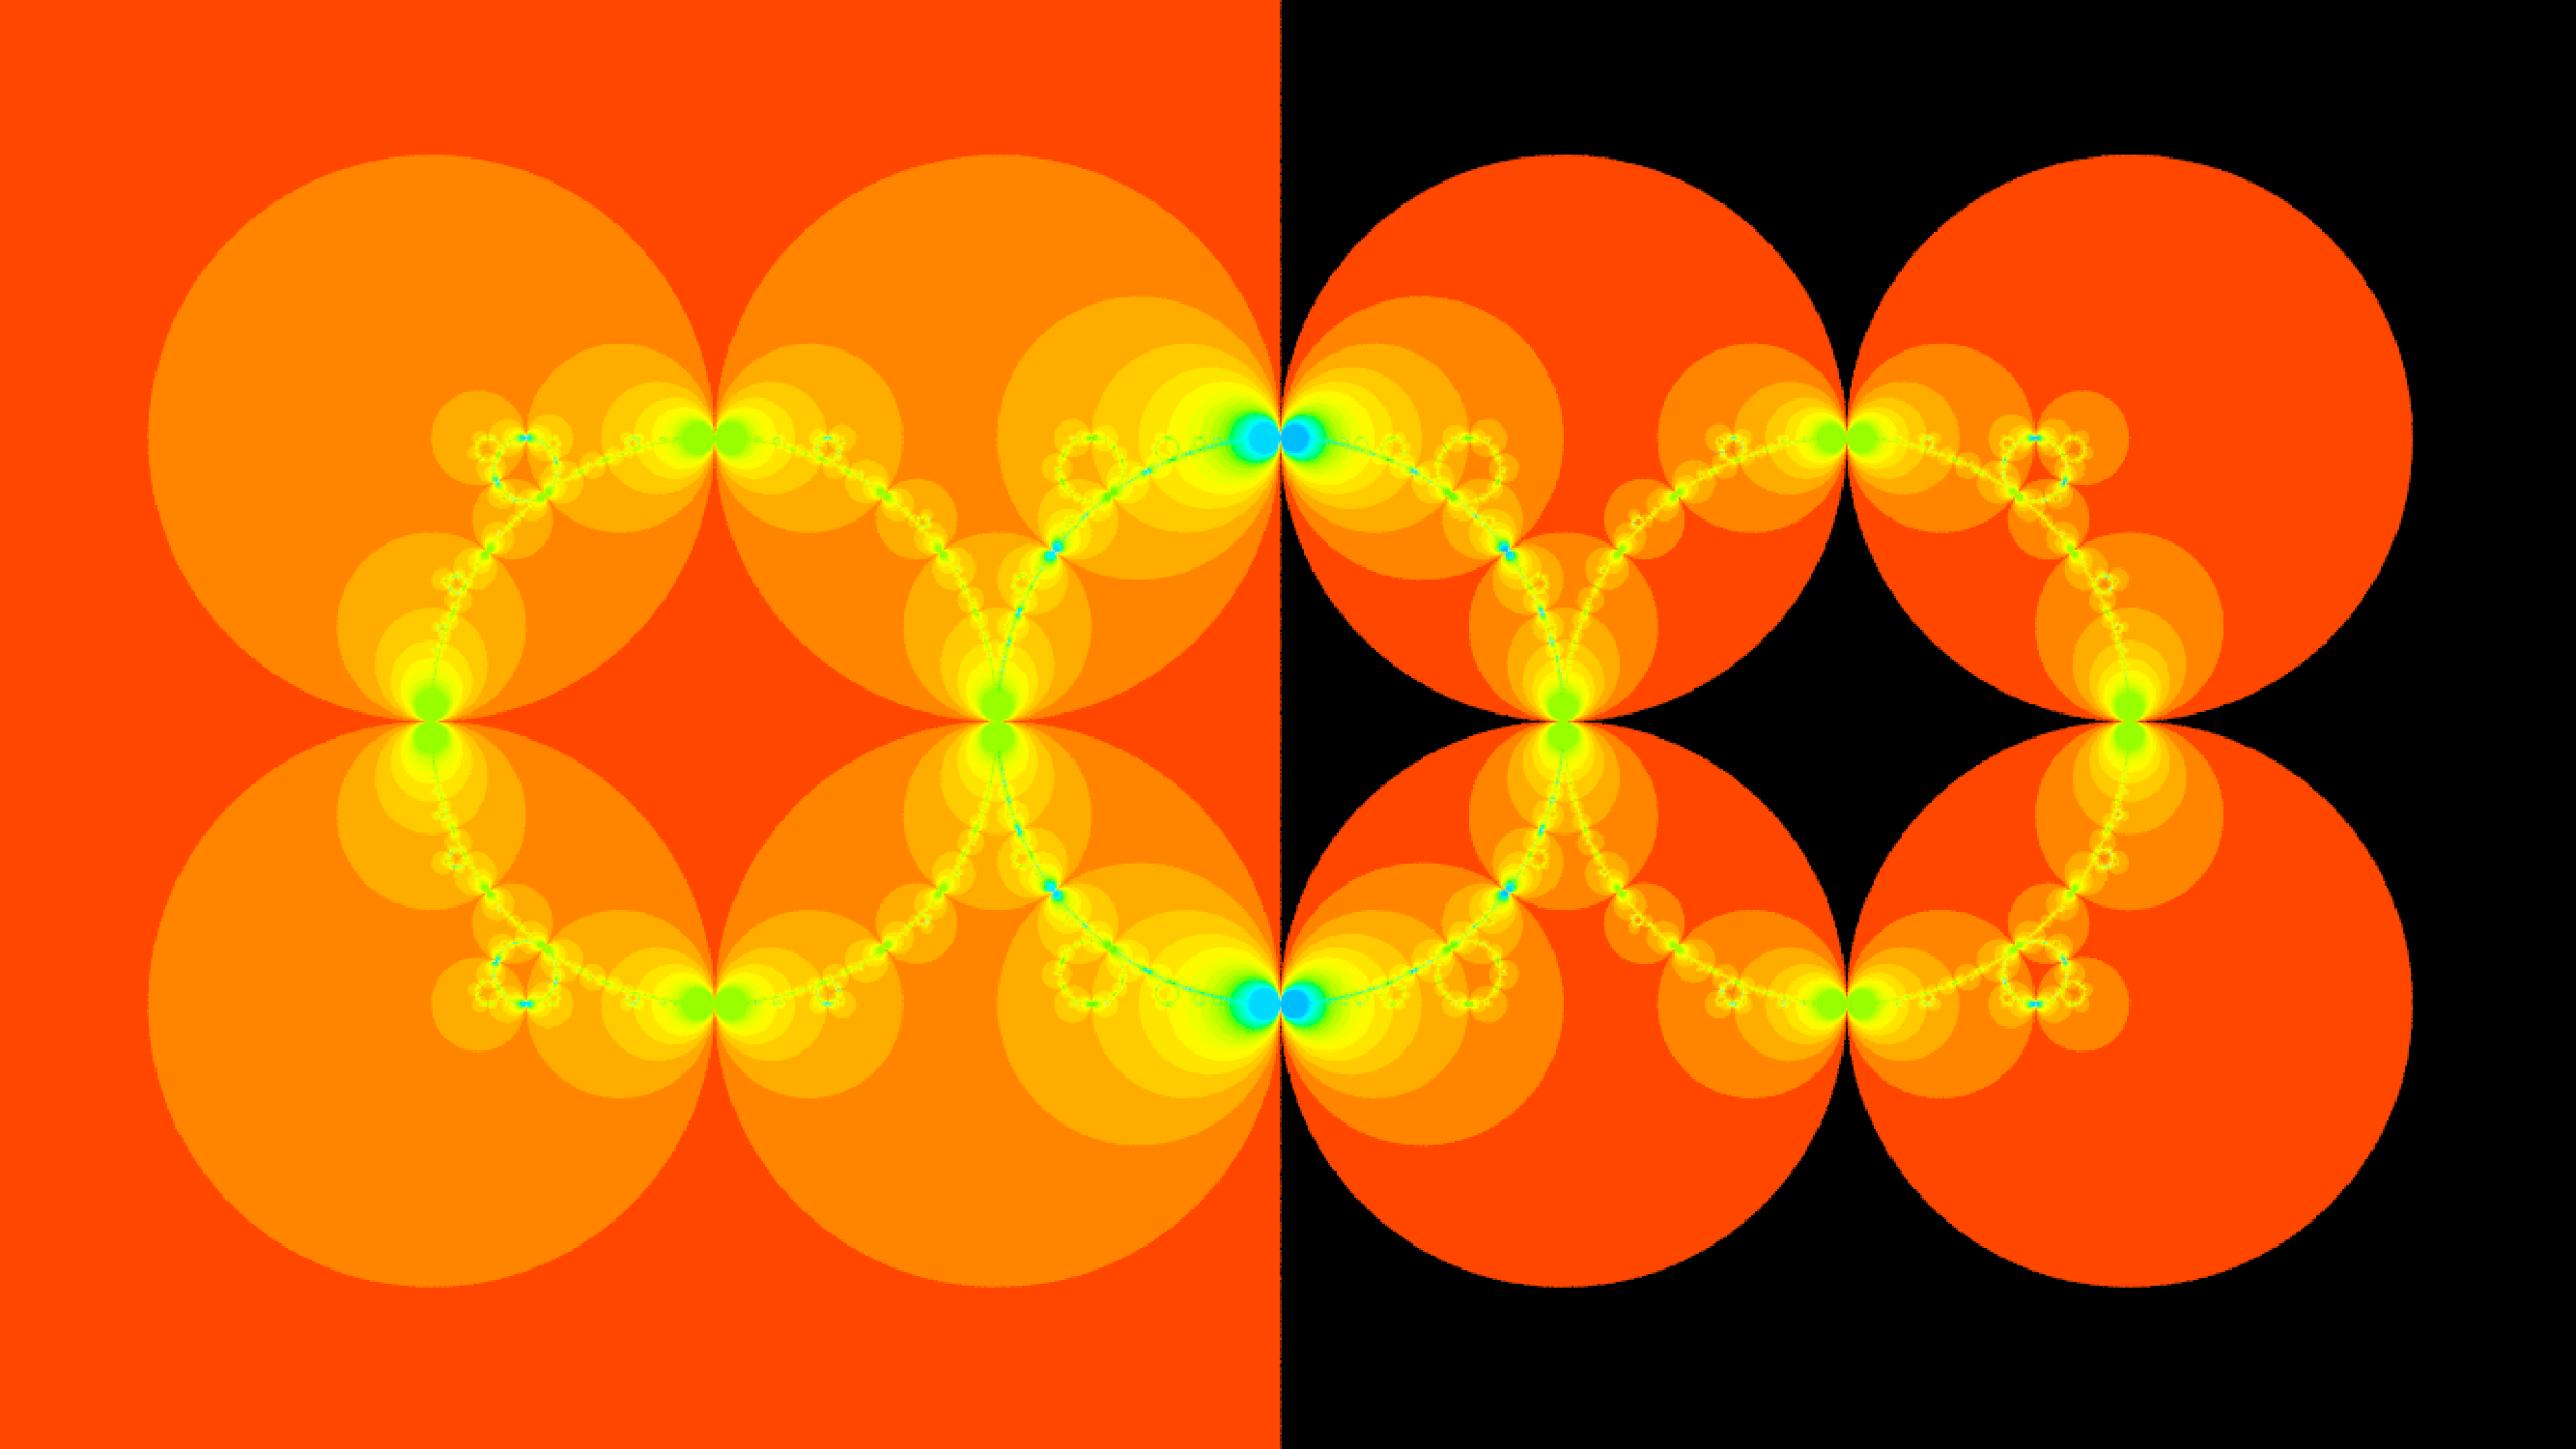
\includegraphics[width=2in, height=2in, keepaspectratio]{../img/klein/2diis/infCircle.pdf}
  \caption{Inversion of the circle with infinite radius}
  \label{fig:infCircle}
 \end{minipage}
 \hspace*{\fill}
 \begin{minipage}[t]{0.3\hsize}
  \center
  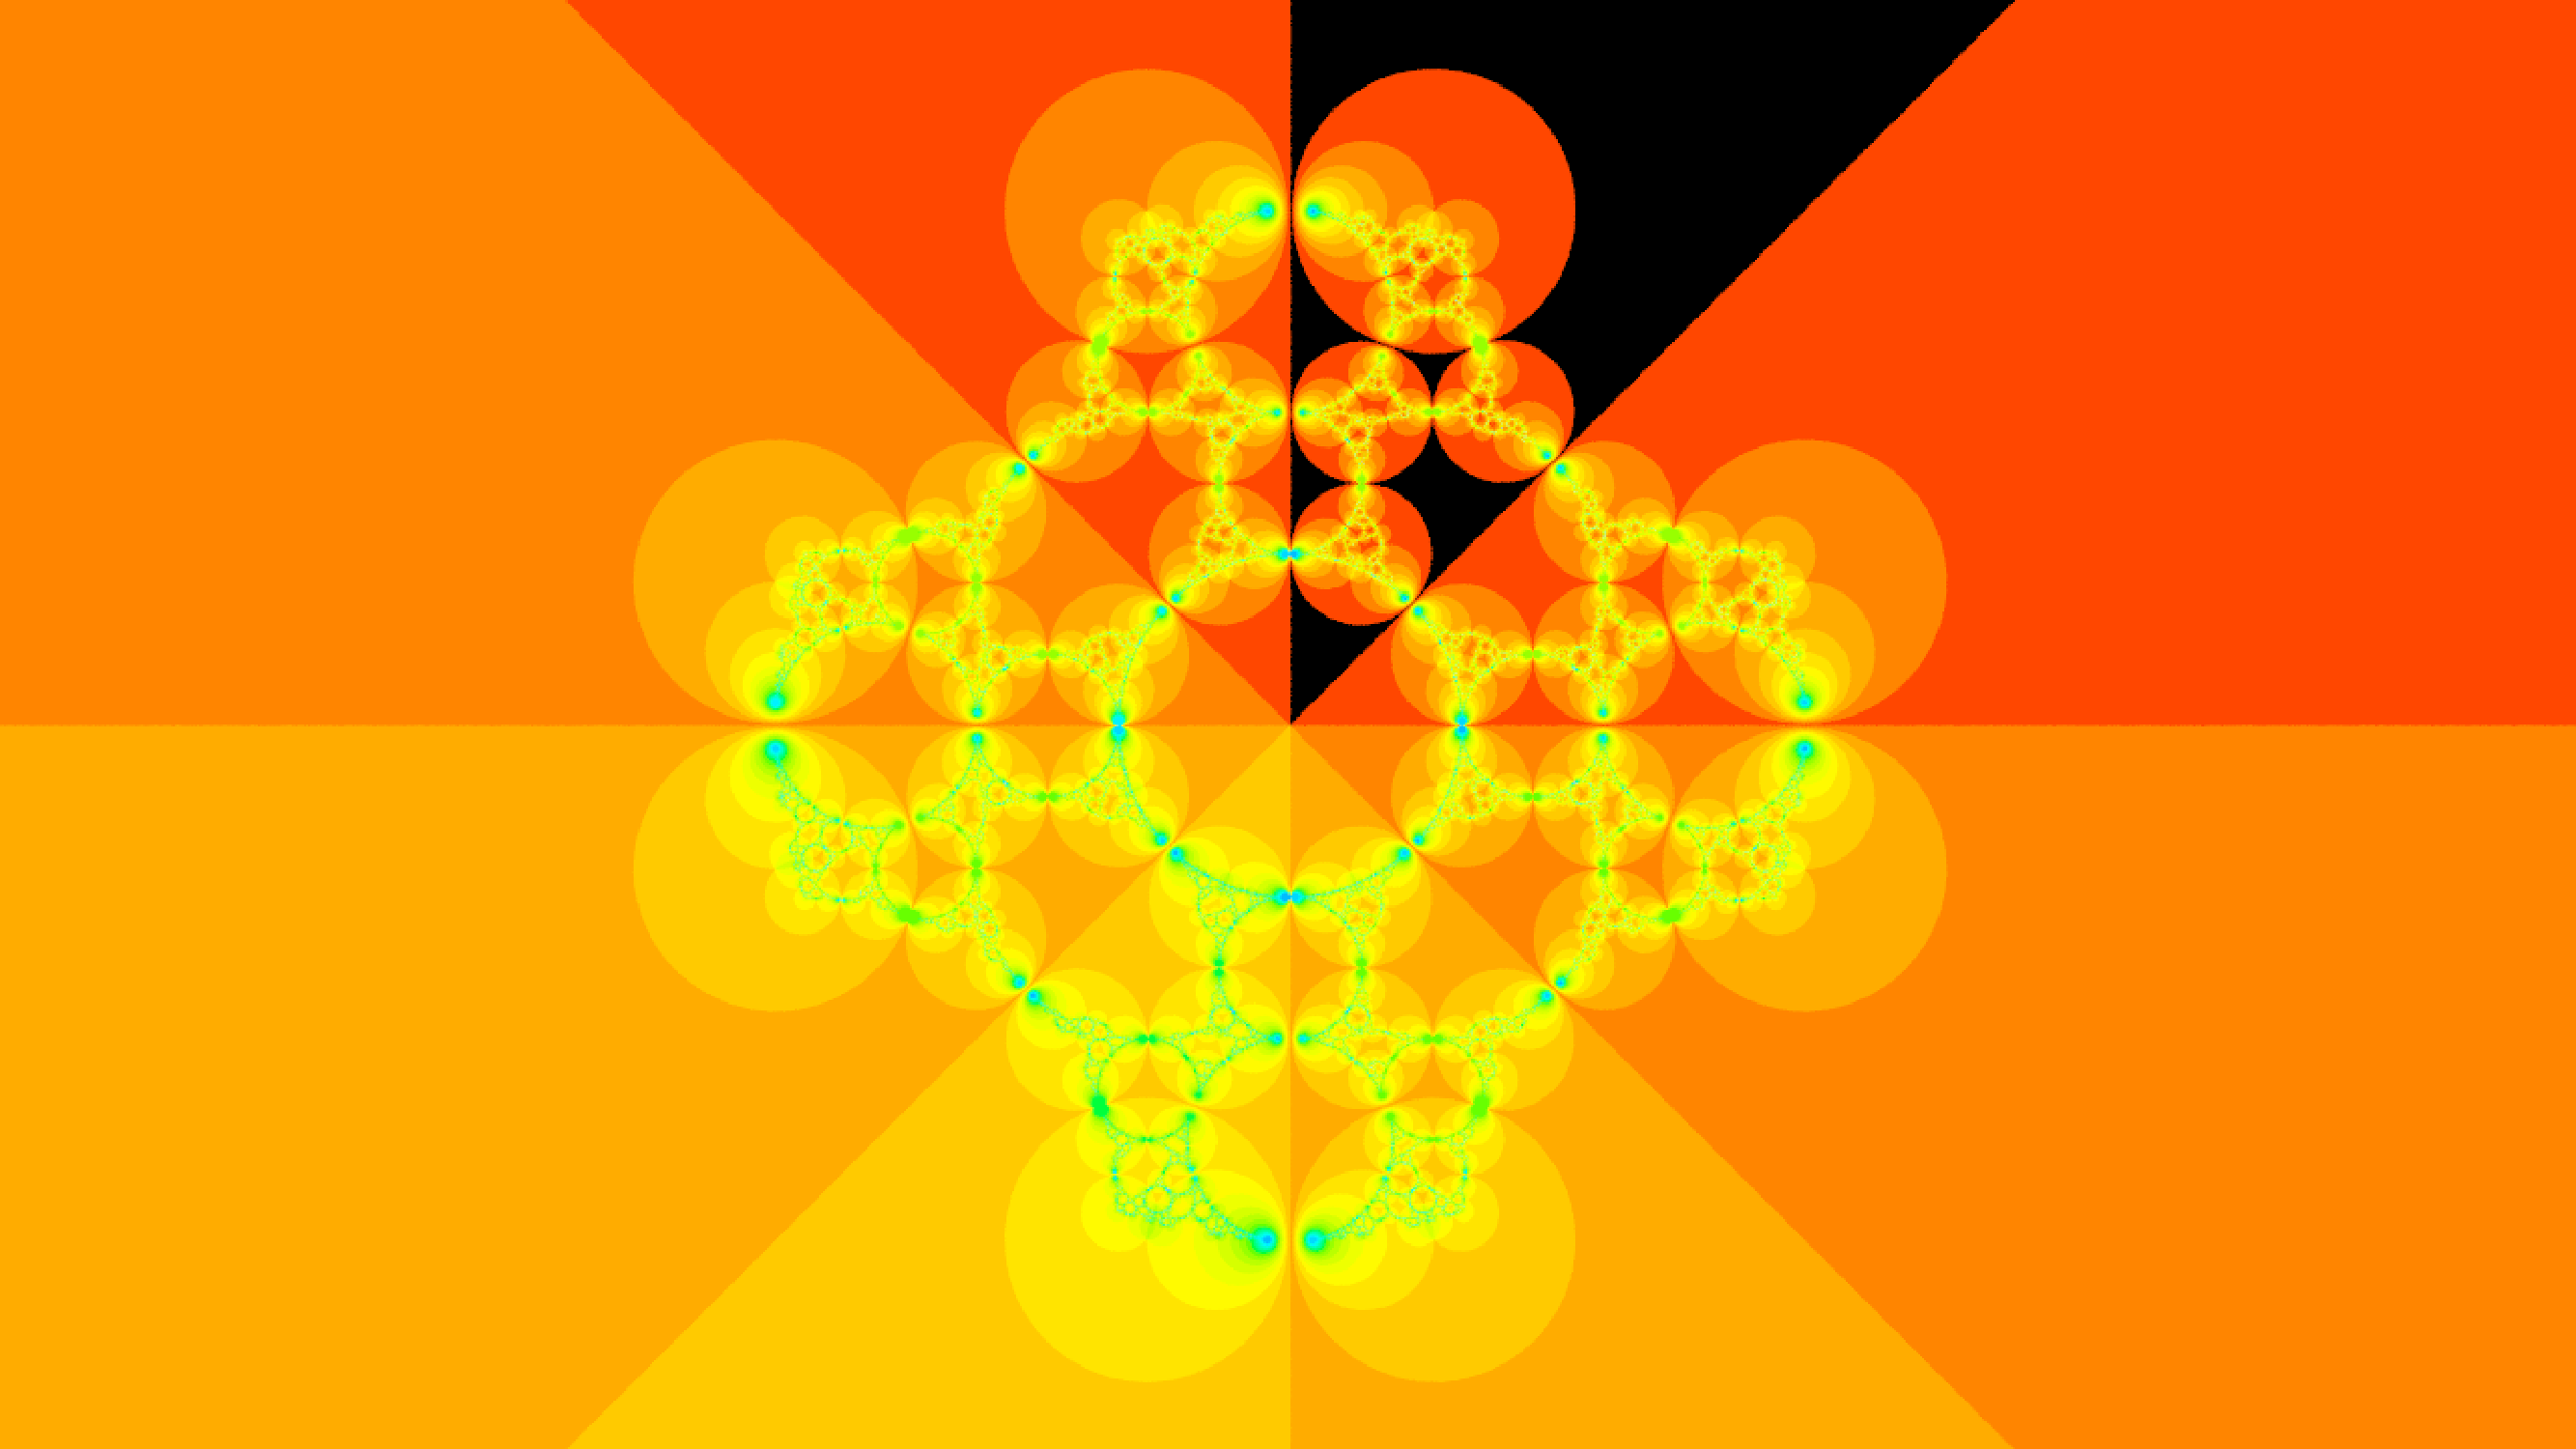
\includegraphics[width=2in, height=2in, keepaspectratio]{../img/klein/2diis/rotation.pdf}
  \caption{Rotation}
  \label{fig:rotation}
 \end{minipage}
 \hspace*{\fill}
 \begin{minipage}[t]{0.3\hsize}
  \center
  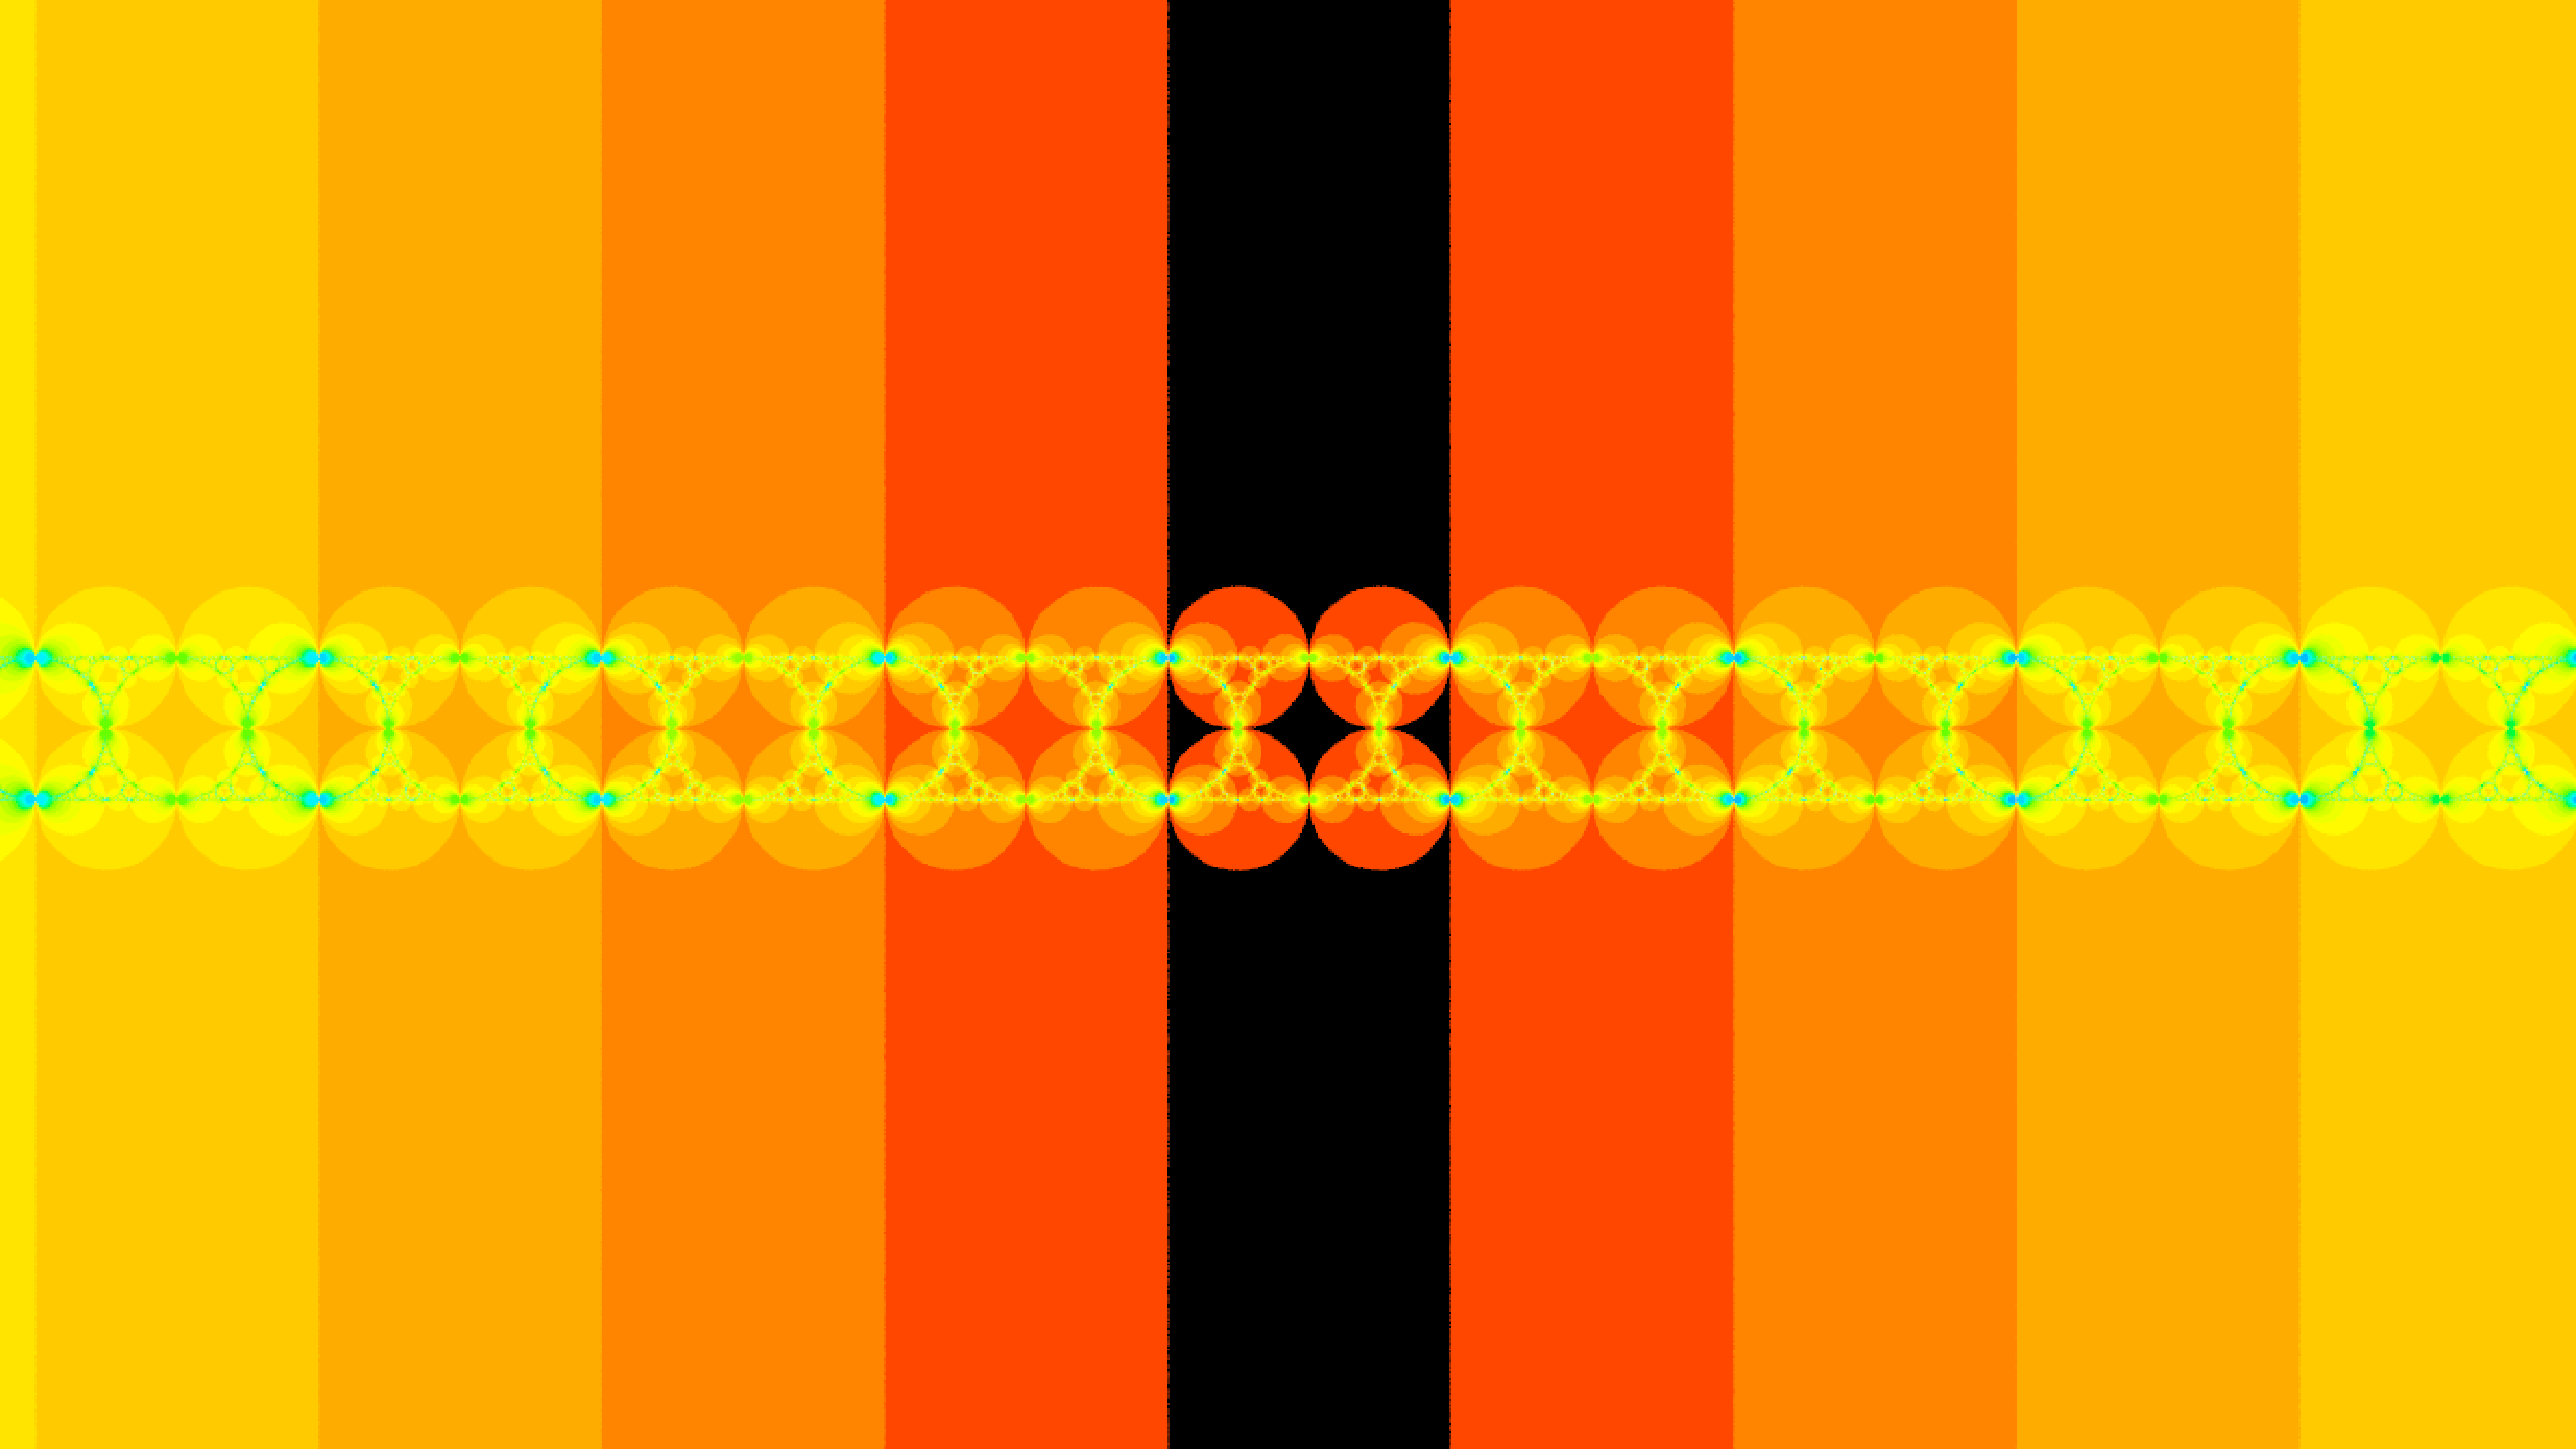
\includegraphics[width=2in, height=2in, keepaspectratio]{../img/klein/2diis/translation.pdf}
  \caption{Parallel translation}
  \label{fig:translation2d}
 \end{minipage}
\end{figure}

\begin{figure}[h!tbp]
 \begin{minipage}[]{0.65\hsize}
  \begin{minipage}[]{0.22\hsize}
   \center
   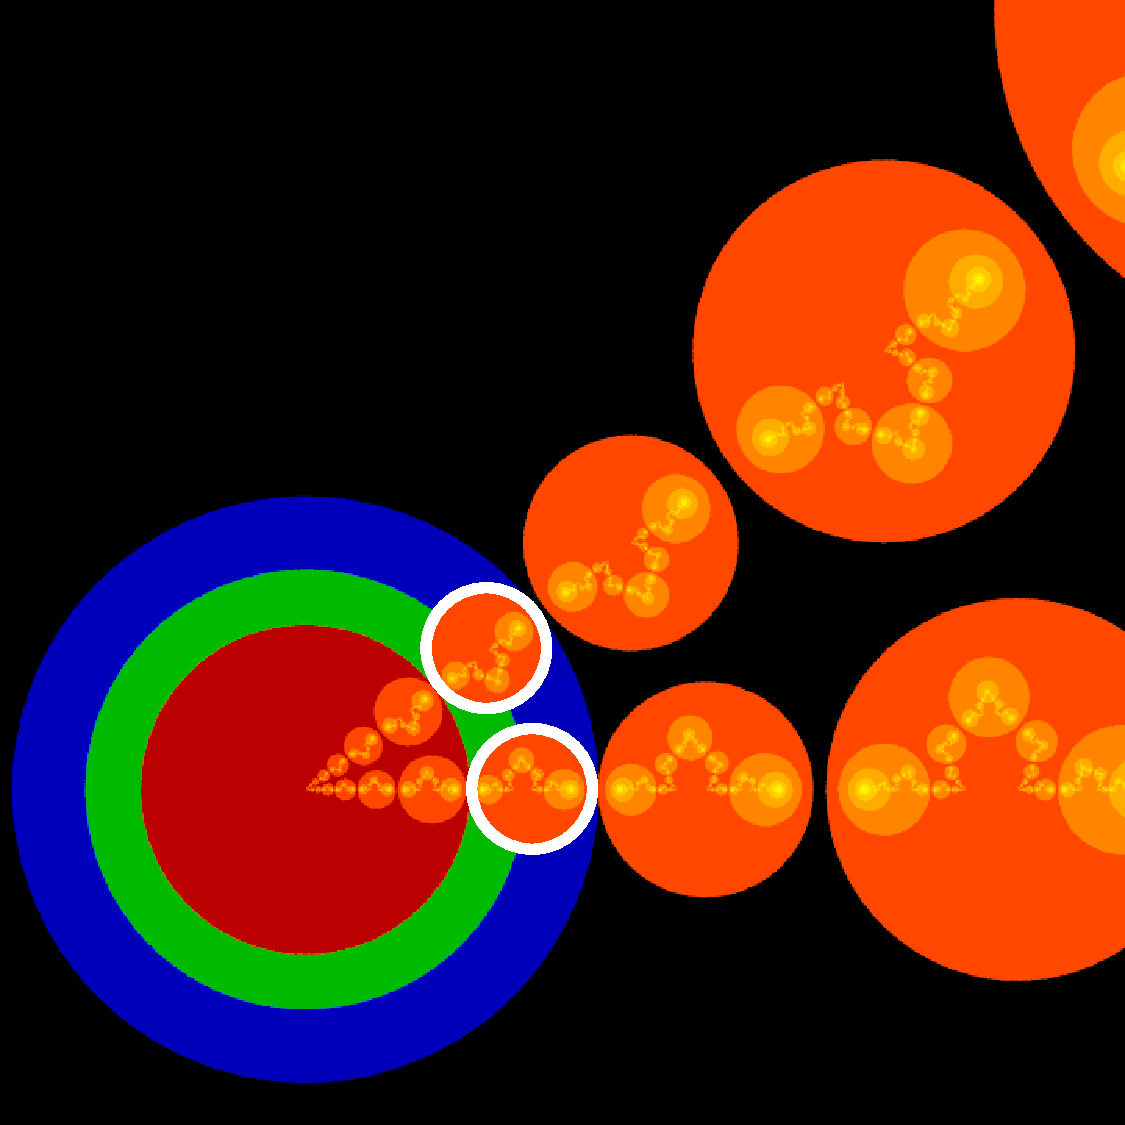
\includegraphics[width=1.5in, height=1.5in, keepaspectratio]{../img/klein/2diis/scalingEdged.pdf}
   \subcaption{Scaling}
   \label{fig:scaling2d}
  \end{minipage}
 \hspace*{\fill}
  \begin{minipage}[]{0.22\hsize}
   \center
   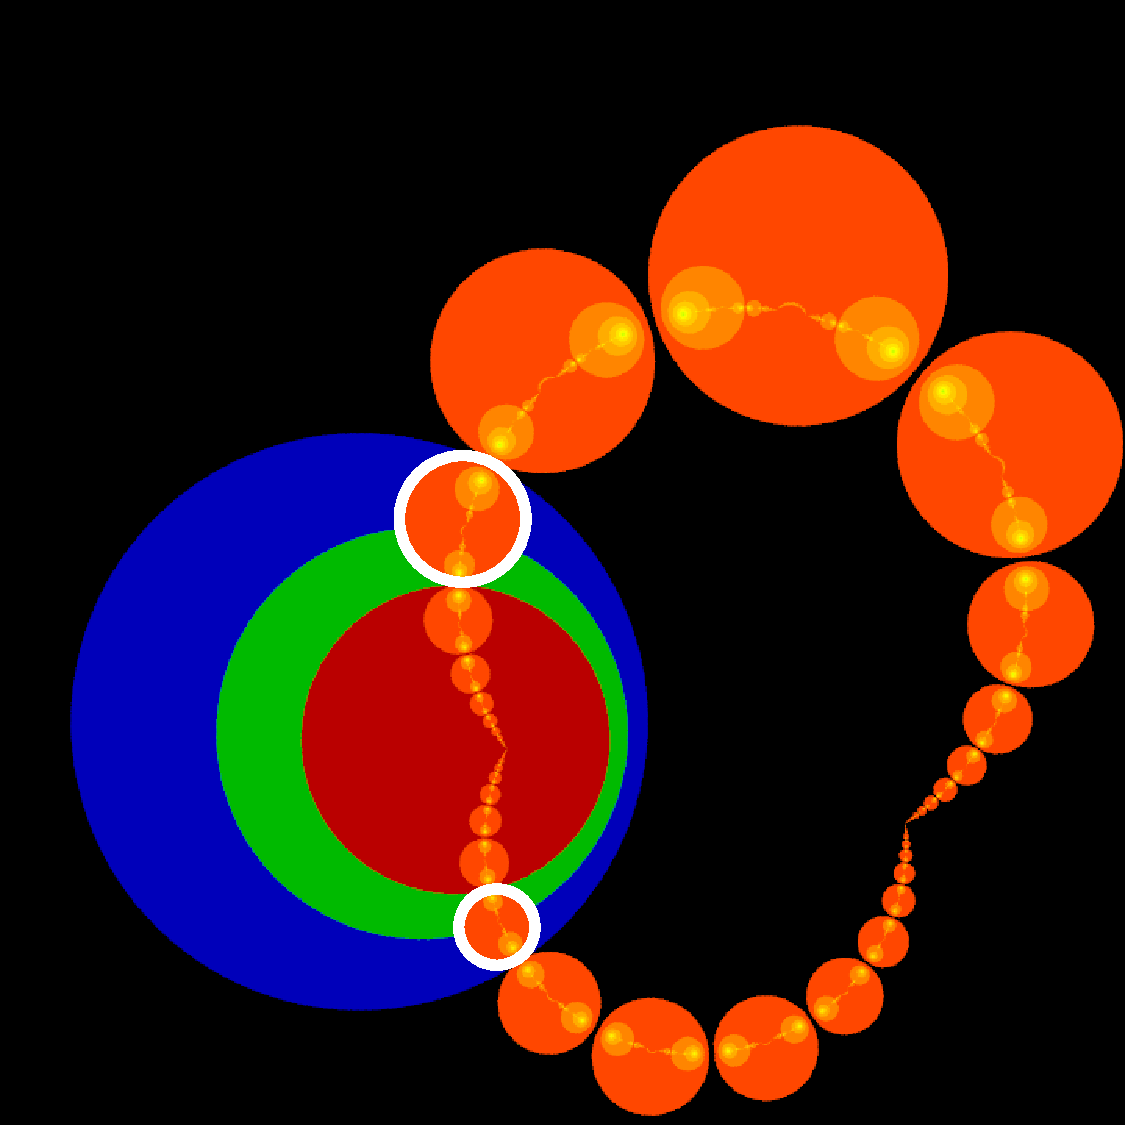
\includegraphics[width=1.5in, height=1.5in, keepaspectratio]{../img/klein/2diis/hyperbolicEdged.pdf}
   \subcaption{Hyperbolic}
   \label{fig:hyperbolic2d}
  \end{minipage}
 \hspace*{\fill}
  \begin{minipage}[]{0.22\hsize}
   \center
   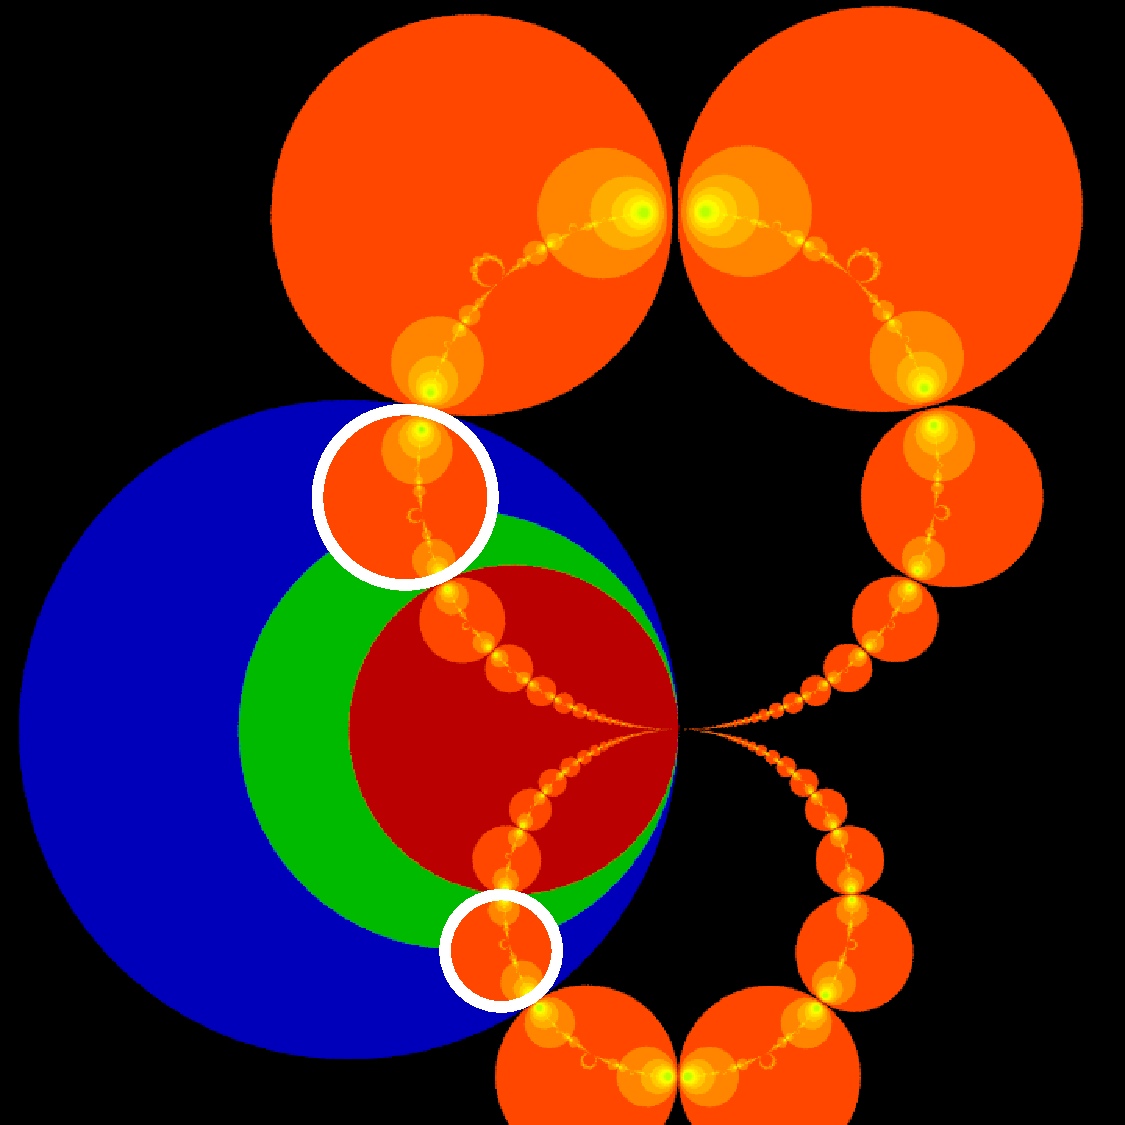
\includegraphics[width=1.5in, height=1.5in, keepaspectratio]{../img/klein/2diis/parabolicEdged.pdf}
   \subcaption{Parabolic}
   \label{fig:parabolic2d}
  \end{minipage}
  \caption{Composition of two circles}
 \end{minipage}
 \hspace*{\fill}
 \begin{minipage}[]{0.22\hsize}
  \center
  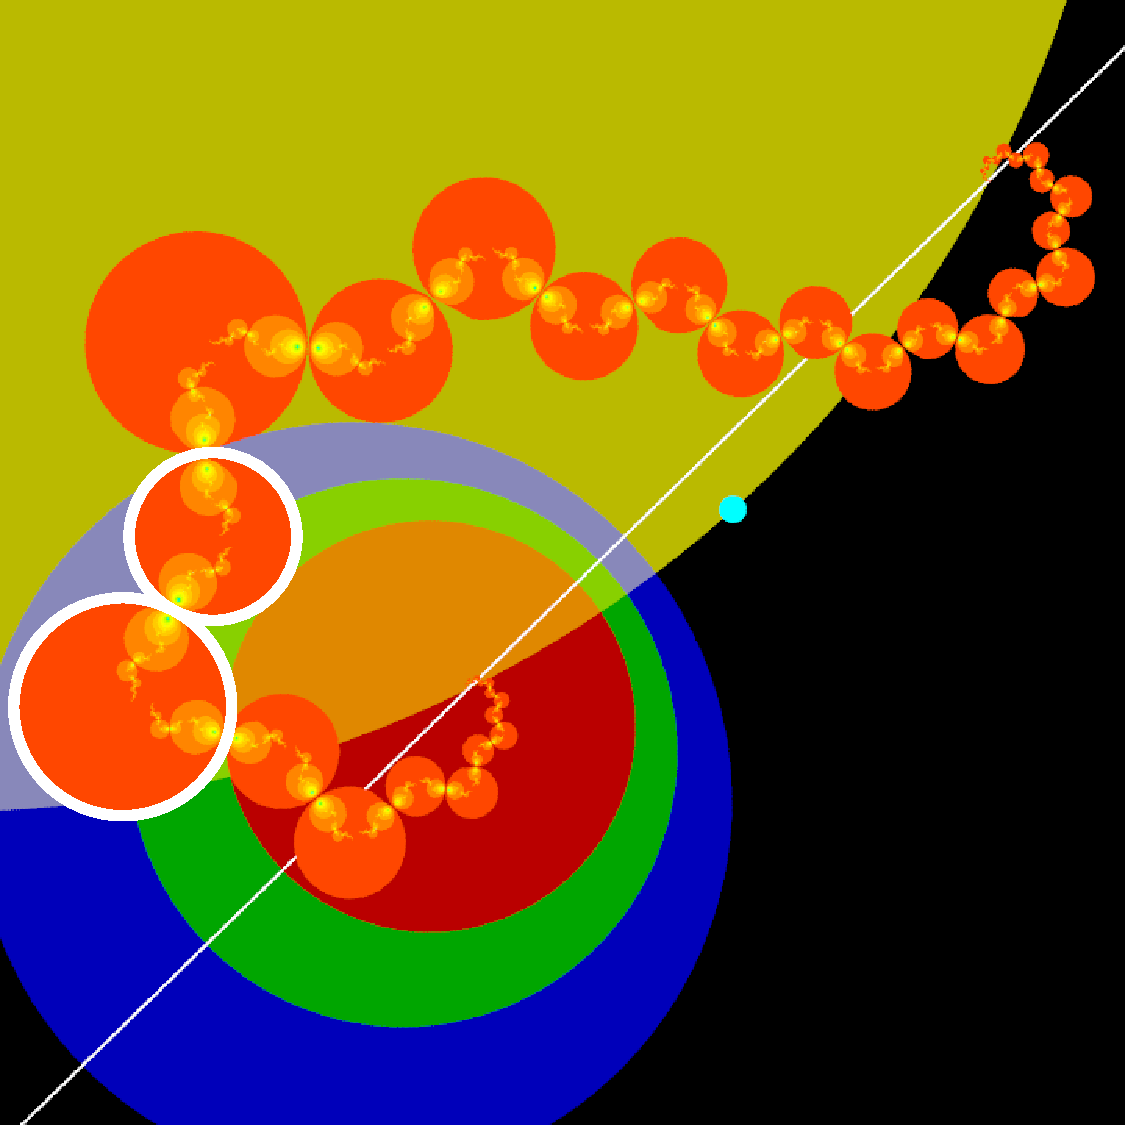
\includegraphics[width=1.5in, height=1.5in, keepaspectratio]{../img/klein/2diis/loxodromicEdged.pdf}
  \caption{Loxodromic transformation}
  \label{fig:loxodromic2d}
 \end{minipage}
\end{figure}

\subsubsection{3D Generators}
ほとんどの三次元の生成元は二次元の生成元から自然に導くことができる.

\noindent\textbf{Simple Inversion.}
二次元の場合と同様に球の反転単体はメビウス変換ではなく, 二つの球のペアに
よる反転がメビウス変換である.
しかし, ここではこれもメビウス変換として扱う.

l\noindent\textbf{Inversion of a Sphere with Infinite Radius}
半径が無限大の球による反転は平面による反転と表すことができる.
図\ref{fig:infSphereGen}では青い板が半径が無限の球を表現している.
図\ref{fig:infSphereOrb}における軌道の右側はこの板によって左側へと
移されることによって左右に対称性をみることができる.

\noindent\textbf{Rotation}
二次元の場合と同様にして,互いに交わる二つの平面の反転によって
回転を表すことができる.
回転軸は二枚の平面の交線で,なす角の二倍が回転角となる.
図\ref{fig:rotation3d}では180度の回転を示した.

\noindent\textbf{Parallel Translation}
二つの平行な平面の組は平面の法線方向への平行移動を表わす.
図\ref{fig:translation3d}のような生成元は無限遠点に固定点
をもつ放物型変換である.

\noindent\textbf{Compound Parabolic}
更に, 三次元では平行移動の軌道に捻りを加えることができる.
図\ref{fig:compParabolic}では軌道に平行移動の元が適用されるたびに回転
が加えられていることがわかる.
この生成元は\emph{複合放物型変換}(\textit{Compound Parabolic})とよばれる.

\noindent\textbf{Composition of Two Spheres}

二次元の場合と同様に二つの球の反転を組み合わせた生成元を定義することができる.
図\ref{fig:loxoGen3d}に示される赤い球を$S1$, 黄緑の球を$S2$,
青い球を$S1'$とよぶとき,写像$G$は二次元と同様に以下のようになる.
\begin{align*}
G =
\begin{cases}
 I_{S2} \circ I_{S1} & (\text{The point is inside of } S1) \\
 I_{S1} \circ I_{S2} & (\text{The point is outside of }S1')
\end{cases}
\end{align*}
$S1$と$S2$に接触がない場合,この生成元は斜航型変換となる.
軌道は図\ref{fig:loxoOrb3d}に示した.
$S1$と$S2$が一点で接触し時, 放物型変換となる.
その接点が固定点となる.
図\ref{fig:parabolic3d}において球の軌道は固定点ので接触していることがわかる.

\noindent\textbf{Compound Loxodromic}
最後に, $S1$と$S2$に直交する二つの球を追加する.
図\ref{fig:compLoxoGen}に示される桃色の球を$S3$, 黄色の球を$S4$,
3つの制御点を$P$,$Q1$,$Q2$とよぶ.
球は4つの点により決定される.
$P'$と$P''$を$P$の$S1$と$S2$の反転による像とすると,
$G$は以下のようになる.
\begin{align*}
S3 = Sphere(P, P', P'', Q1) \quad
S4 = Sphere(P, P', P'', Q2) \\
G =
\begin{cases}
 (I_{S4} \circ I_{S3}) \circ (I_{S1} \circ I_{S2}) & (\text{The point is inside of } S1) \\
 (I_{S2} \circ I_{S1}) \circ (I_{S3} \circ I_{S4}) & (\text{The point is
 outside of } S1')\\
\end{cases}
\end{align*}
$S3$と$S4$の反転の組み合わせは回転を表す.
図\ref{fig:compLoxoOrb}では, 二次元における斜航型変換のような捻じれた
軌道をみることができる.
この生成元を\emph{複合斜航型変換}(Compound Loxodromic)とよぶ.


\begin{figure}[h!tbp]
 \begin{minipage}[t]{0.49\hsize}
  \begin{subfigure}{0.24\textwidth}
   \begin{center}
    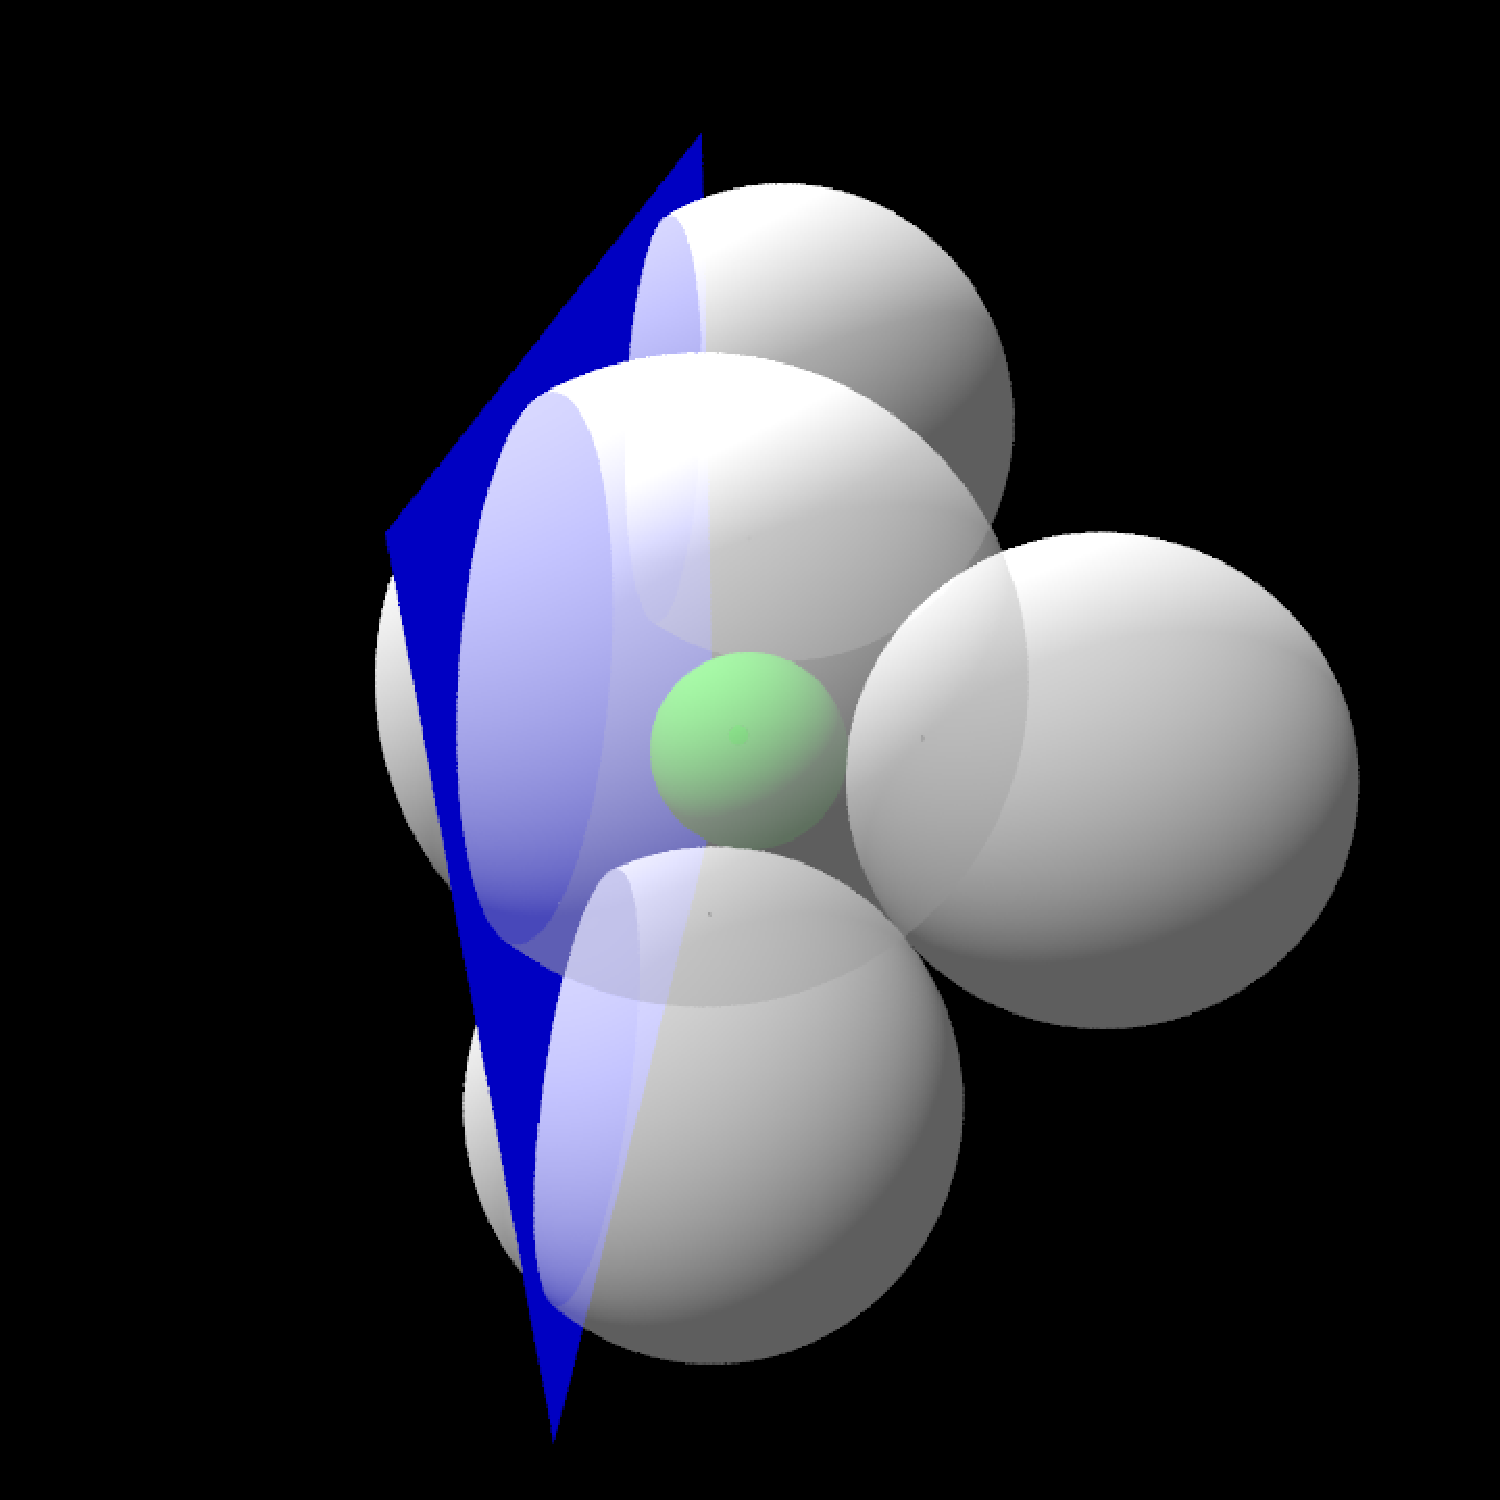
\includegraphics[width=1.5in, height=1.5in, keepaspectratio]{../img/klein/3diis/infSphereGen.pdf}
    \caption{Generator}
    \label{fig:infSphereGen}
   \end{center}
  \end{subfigure}
  \hspace*{\fill}
  \begin{subfigure}{0.24\textwidth}
   \begin{center}
    \includegraphics[width=1.5in, height=1.5in, keepaspectratio]{../img/klein/3diis/infSphereOrbit.pdf}
    \caption{Orbit}
    \label{fig:infSphereOrb}
   \end{center}
  \end{subfigure}
  \hspace*{\fill}
  \caption{Inversion of the Sphere with infinite radius}
  \label{fig:infSphere}

 \end{minipage}
 \hspace*{\fill}
 \begin{minipage}[t]{0.49\hsize}

  \begin{subfigure}{0.24\textwidth}
   \begin{center}
    \includegraphics[width=1.5in, height=1.5in, keepaspectratio]{../img/klein/3diis/rotationGen.pdf}
    \caption{Generator}
    \label{fig:rotationGen}
   \end{center}
  \end{subfigure}
  \hspace*{\fill}
  \begin{subfigure}{0.24\textwidth}
   \begin{center}
    \includegraphics[width=1.5in, height=1.5in, keepaspectratio]{../img/klein/3diis/rotationOrb.pdf}
    \caption{Orbit}
    \label{fig:rotationOrb}
   \end{center}
  \end{subfigure}
  \hspace*{\fill}
  \caption{Rotation}
  \label{fig:rotation3d}
 \end{minipage}
\end{figure}

\begin{figure}[h!tbp]
 \begin{minipage}{0.49\hsize}
  \begin{subfigure}{0.24\textwidth}
   \begin{center}
    \includegraphics[width=1.5in, height=1.5in, keepaspectratio]{../img/klein/3diis/translationGen.pdf}
    \caption{Generator}
    \label{fig:translationGen}
   \end{center}
  \end{subfigure}
 \hspace*{\fill}
 \begin{subfigure}{0.24\textwidth}
  \begin{center}
   \includegraphics[width=1.5in, height=1.5in, keepaspectratio]{../img/klein/3diis/translationOrbit.pdf}
   \caption{Orbit}
    \label{fig:translationOrb}
  \end{center}
 \end{subfigure}
 \hspace*{\fill}
\caption{Parallel translation}
 \label{fig:translation3d}

 \end{minipage}
 \begin{minipage}{0.49\hsize}
  \begin{subfigure}{0.24\textwidth}
   \begin{center}
    \includegraphics[width=1.5in, height=1.5in, keepaspectratio]{../img/klein/3diis/compParabolicGen.pdf}
    \caption{Generator}
    \label{fig:compParabolicGen}
   \end{center}
  \end{subfigure}
 \hspace*{\fill}
 \begin{subfigure}{0.24\textwidth}
  \begin{center}
   \includegraphics[width=1.5in, height=1.5in, keepaspectratio]{../img/klein/3diis/compParabolicOrb.pdf}
   \caption{Orbit}
   \label{fig:compParabolicOrb}
  \end{center}
 \end{subfigure}
 \hspace*{\fill}
\caption{Compound parabolic transformation}
 \label{fig:compParabolic}
 \end{minipage}
\end{figure}

\begin{figure}[h!tbp]

  \begin{subfigure}{0.24\textwidth}
   \begin{center}
    \includegraphics[width=1.5in, height=1.5in, keepaspectratio]{../img/klein/3diis/loxoGenSimple.pdf}
    \caption{Generator}
    \label{fig:loxoGen3d}
   \end{center}
  \end{subfigure}
 \hspace*{\fill}
  \begin{subfigure}{0.24\textwidth}
   \begin{center}
    \includegraphics[width=1.5in, height=1.5in, keepaspectratio]{../img/klein/3diis/loxoOrbSimple.pdf}
    \caption{Orbit}
    \label{fig:loxoOrb3d}
   \end{center}
  \end{subfigure}
 \hspace*{\fill}
 \begin{subfigure}{0.24\textwidth}
  \begin{center}
   \includegraphics[width=1.5in, height=1.5in, keepaspectratio]{../img/klein/3diis/loxoOrbSch.pdf}
   \caption{Orbit}
   \label{fig:loxoOrbSch3d}
  \end{center}
 \end{subfigure}

  \caption{Loxodromic transformation}
  \label{fig:loxodromic3d}

\end{figure}

\begin{figure}[h!tbp]
 \begin{minipage}{0.49\hsize}
  \begin{subfigure}{0.24\textwidth}
   \begin{center}
    \includegraphics[width=1.5in, height=1.5in, keepaspectratio]{../img/klein/3diis/parabolicGen.pdf}
    \caption{Generator}
    \label{fig:parabolicGen3d}
   \end{center}
  \end{subfigure}
 \hspace*{\fill}
 \begin{subfigure}{0.24\textwidth}
  \begin{center}
   \includegraphics[width=1.5in, height=1.5in, keepaspectratio]{../img/klein/3diis/parabolicOrb.pdf}
   \caption{Orbit}
   \label{fig:parabolicOrb3d}
  \end{center}
 \end{subfigure}
  \hspace*{\fill}
  \caption{Parabolic transformation}
  \label{fig:parabolic3d}
 \end{minipage}
 \begin{minipage}{0.49\hsize}
  \begin{subfigure}{0.24\textwidth}
   \begin{center}
    \includegraphics[width=1.5in, height=1.5in, keepaspectratio]{../img/klein/3diis/compLoxoGen.pdf}
    \caption{Generator}
    \label{fig:compLoxoGen}
   \end{center}
  \end{subfigure}
 \hspace*{\fill}
 \begin{subfigure}{0.24\textwidth}
  \begin{center}
   \includegraphics[width=1.5in, height=1.5in, keepaspectratio]{../img/klein/3diis/compLoxoOrb.pdf}
   \caption{Orbit}
   \label{fig:compLoxoOrb}
  \end{center}
 \end{subfigure}
  \hspace*{\fill}
  \caption{Compound loxodromic transformation}
  \label{fig:compLoxo}
 \end{minipage}
\end{figure}

\begin{figure}[h!tbp]
 \begin{minipage}[t]{0.24\hsize}
  \begin{center}
   \includegraphics[width=1.5in, height=1.5in, keepaspectratio]{../img/klein/2diis/translationMod.pdf}
  \end{center}
  \caption{Parallel translation}
  \label{fig:translationMod}
 \end{minipage}
 \hspace*{\fill}
 \begin{minipage}[t]{0.24\hsize}
  \begin{center}
   \includegraphics[width=1.5in, height=1.5in, keepaspectratio]{../img/klein/2diis/parabolicMod.pdf}
  \end{center}
  \caption{Inverted parabolic generator}
  \label{fig:parabolicMod}
 \end{minipage}
 \hspace*{\fill}
 \begin{minipage}[t]{0.24\hsize}
   \begin{center}
    \includegraphics[width=1.5in, height=1.5in, keepaspectratio]{../img/klein/2diis/hyperbolicMod.pdf}
   \end{center}
   \caption{Inverted hyperbolic generator}
   \label{fig:loxodromicMod}
 \end{minipage}
  \hspace*{\fill}
 \begin{minipage}[t]{0.24\hsize}
   \begin{center}
    \includegraphics[width=1.5in, height=1.5in, keepaspectratio]{../img/klein/2diis/loxodromicModRotation.pdf}
   \end{center}
   \caption{Inverted loxodromic generator}
   \label{fig:loxodromicRotationMod}
  \hspace*{\fill}
 \end{minipage}
\end{figure}

\subsubsection{Optimization}

いくつかの反転で構成された写像は適切な共役をとることによって, 最適化する
ことができる.
最適化された写像は点を一度の操作で基本領域に移動させることができる.
この節では, 二次元の生成元の最適化についてまとめる.

\noindent\textbf{Parallel Translation.}
まずは図\ref{translation2d}と同様の平行な二直線の組による平行移動を考える.
繰り返し反転を適用する代わりに, 剰余を用いて点を移すことができる.

まず始めに, 与えられた点を平行移動と回転を用いて,
平行な二直線がX軸に垂直に, 片方の直線がY軸に沿うようにする.
これらの変換が共役変換となる.
共役変換で移された直線は図\ref{translationMod}に示した.
$w$を二直線の距離, $i$を平行移動によって移された半径無限の円の指数,
$P$を写像に与えられた点,
$P'$を写像によって移された点, $d$と$d'$をY軸からの距離とする.
$d$を$w$で割ることにより, 剰余$d'$と商$i$を得る.
最後に$d'$を用いて$P'$を計算し, これを共役変換で元の座標に戻す.
以上の操作を一度行うことで,平面上の全ての点を基本領域に移すことができる.

\noindent\textbf{Parabolic.}
次に図のような放物型変換を考える.
まず共役変換$T$をこの変換の固定点を中心とする円の反転とする.
$T$を$C1,C2,C1'$に対して適用すると, 固定点は無限遠点に移るので, 三本の平行な直
線を得ることができる.
これらの直線を$TC1, TC2, TC1'$とよぶ.
図ではこれらの直線が示されている.
赤の直線$TC1$と青の直線$TC1'$が平行移動を表す.
写像の過程は以下のようになる.
まず, $T$を与えられた点$P$に適用し, $T(P)$を得る.
そして, $T(P)$を平行移動と同様にして移し, $P'$を得る.
最後にもう一度$T(= T^{-1})$を$P'$に適用する.

\noindent\textbf{Loxodromic}
最後に図のような双曲型変換を考える.
共役変換$T$を片方の固定点を中心にもつ円に関する反転とする.
$T$を$C1, C2, C1'$に適用した像を$TC1, TC2, TC1'$とよび, これらは, もう一
方の固定点の反転した像を中心にもつ同心円となる.
これは実数倍を表す.
図において, $P$を写像に与えられた点, $P'$を写像された点, $r$と$r'$を
$TC1$と$TC1'$の半径, $d$と$d'$を$TC1$からの距離, $k$を倍数, $q$を
$exponential ciefficient$,  $i$を円列の指数とする.
これらは以下のように計算される.
 \begin{math}
  k = \frac{r'}{r},
  q = \log_{k} \frac{d}{r},
  d' = r \cdot k^{fracionalPart(q)},
  i = floor(q).
 \end{math}
我々は$d'$を用いて$P'$を計算することができる.

また, 図のような双曲型変換であるとき, $T$を$L$と$C3$にも適用し, その像を
$TL$と$TC3$とよぶ.
図は複素数によるスケーリングを表している.
白い直線$TL$と黄色の直線$TC3$は同心円の中心で交わっている.
$P'$を得た後で回転を与えて$P''$を得る.
$TL$と$TC3$のなす角を$\theta$, 回転角を$\varphi$とすると, $\varphi$は
$\varphi = 2 \theta i$で計算することができる.

まず, $T$を与えられた点$P$に適用し, $T(P)$を得る.
そして, $d'$を用いて$P'$を計算する.
もしも交差する直線があれば, $P'$を$\varphi$回転させ, $P''$を得る.
最後にもう一度$T$を$P'$もしくは$P''$に適用する.

\subsection{Other Topics}

この節では, その他のレンダリング手法とクライン群の研究の中でも興味深い図
像を見ることができる先行研究を紹介する.

\subsubsection{Other Rendering Methods}
Aaron MontagはIterated Inversion Systemを拡張したHyperbolic Iterated
Function Systemによる極限集合の描画を提案している\cite{hyperbolicIFS}
\footnote{Kleinian Groups WebGL:
 \url{https://www-m10.ma.tum.de/bin/view/Lehrstuhl/AaronMontagKleinian}}.

また, Jos Ley・Knightyはマスキット群におけるEscape-timeアルゴリズムの式
とDistance Estimationを考案した
\footnote{An escape time algorithm for Kleinian group limit set:\\ \quad
\quad \url{http://www.fractalforums.com/3d-fractal-generation/an-escape-tim-algorithm-for-kleinian-group-limit-sets/}}.
荒木・糸\cite{maskit}の考えた群と同様に, 一方に平行移動を含む2つの放物型変換による群を考えている.
この方法を用いると, 二次元だけでなく,三次元の図像も高速に描画することができる.
詳細なアルゴリズムに関しては, Jos Leyがまとめている
\footnote{Mathematical Imagery, An escape-time algorithm for a family of
Kleinian groups:\\ \quad \quad \url{http://www.josleys.com/article_show.php?id=221}}.

\subsubsection{Quasi Fuchsian 3-Dimensional Fractals}

阿原・荒木は擬フックス群を三次元に拡張した4次元クライン群を考案した
\cite{sphairahedra}\cite{sphairahedraJa}.
これはQuasi Fuchsian 3-Dimensional Fractalsとよばれ,
前述のフラクタルコミュニティに大きな影響を与えたといわれている.
荒木はこのフラクタル図形の物質化についてまとめている\cite{materializing}.
数学的な事項については2016年に蔭山\cite{kageyama}がまとめている.

図\ref{fig:schottky}において, 中央の円盤に囲まれた黒い領域を\emph{円辺形}と
よぶ.
擬フックス群は円辺形を囲む円盤の組から生成元を得ることができる.
そこで円辺形を三次元に拡張した\emph{球面体}を用いることで三次元の擬フッ
クス群を構成することができる.
図\ref{fig:sphairahedra}は6つの球に囲まれた球面体のひとつである.
側面は3つの半径無限大の球に囲まれていると考える.
この球面体をそれを囲む球の反転で移していくことで図\ref{fig:quasiFuchsian}のような形状を得る.
阿原・荒木による動画\footnote{Quasi-fuchsian fractals:
\url{https://www.youtube.com/watch?v=3lcO9zRCv-4}}ではこのフラクタルの構成過程をみることができる.

また, Distance Estimationによる高速描画のアルゴリズムが2012年にKnightyによって開発された
\footnote{Another 3D Kleinian:
 \url{http://www.fractalforums.com/ifs-iterated-function-systems/another-3d-kleinian/}}.

\begin{figure}[htbp]
 \begin{minipage}{0.49\hsize}
  \begin{center}
   \includegraphics[width=3in, height=3in, keepaspectratio]{../img/klein/sphairahedra.pdf}
   \caption{Sphairahedra}
   \label{fig:sphairahedra}
  \end{center}
 \end{minipage}
 \begin{minipage}{0.49\hsize}
  \begin{center}
   \includegraphics[width=3in, height=3in, keepaspectratio]{../img/klein/quasi-fuchsian.pdf}
   \caption{quasi-fuchsian}
   \label{fig:quasiFuchsian}
  \end{center}
 \end{minipage}
\end{figure}

\subsubsection{Other 4-Dimensional Kleinian Groups}

インドラの真珠で紹介されるクライン群は複素平面に作用するメビウス変換から構成されている.
現在このようなクライン群は, ほぼ研究され尽されてしまった.
しかし, 先に述べたように, 三次元空間に作用するメビウス変換を四元数を用い
て定義することができる.
これは$sp^k(1, 1)$と呼ばれ,2x2の四元数行列で表現される.
三次元空間上で捩じりが加わるようなメビウス変換は複合放物型, 複合斜航型と分類
される.
四元数で構成されるメビウス変換とその分類は佐久川による
\cite{sakugawaMaster}や\cite{accidentalParabolic}にまとまっている.

図\ref{fig:sakugawa}は佐久川による複合放物型変換を含む群のレシピによる群
の極限集合を描画したものである.
放物型変換である平行移動に回転が加わることで複合放物型変換となる.

荒木・糸はマスキット群を高次元に拡張した\cite{maskit}
\footnote{4-dimensional Kleinian punctured torus groups:
\url{http://www.math.nagoya-u.ac.jp/~itoken/3d-maskit/3d-maskit.html}}.
論文中では幾何学的性質をうまく使うことで,四元数の計算を避けている.
また, 佐久川はこの群の四元数表示を導出した\cite{sakugawa4d}.

三浦は3つ以上の生成元による4次元クライン群をモジュラー群から構成するこ
とを試みた\cite{miura}.
筆者はこの論文における数値実験と可視化を行った.

\begin{figure}[h!tbp]
 \begin{minipage}{0.49\hsize}
  \center
  \includegraphics[width=3in, height=3in, keepaspectratio]{../img/klein/sakugawa1.pdf}
  \subcaption{}
 \end{minipage}
 \hspace*{\fill}
 \begin{minipage}{0.49\hsize}
  \center
  \includegraphics[width=3in, height=3in, keepaspectratio]{../img/klein/sakugawa2.pdf}
  \subcaption{}
 \end{minipage}
 \begin{minipage}{0.49\hsize}
  \center
  \includegraphics[width=3in, height=3in, keepaspectratio]{../img/klein/sakugawa3.pdf}
  \subcaption{}
 \end{minipage}
 \hspace*{\fill}
 \begin{minipage}{0.49\hsize}
  \center
  \includegraphics[width=3in, height=3in, keepaspectratio]{../img/klein/sakugawa4.pdf}
  \subcaption{}
 \end{minipage}
 \caption{The limit set of the 4-Dimensional Kleinian Groups}
 \label{fig:sakugawa}
\end{figure}

\subsubsection{Once Punctured Torus Groups}

クライン群の部分群である一点穴開きトーラス群({\it Once Punctured Torus Groups})は
和田による{\it OPTi}\footnote{OPTi:
\url{http://delta-mat.ist.osaka-u.ac.jp/OPTi/index.html}}という描画ソフ
トウェアによって大きく研究が進んだ.
描画や離散性判定のためのアルゴリズ
ムが開発者の和田によりまとめられている
\cite{OPTiDrawing}\cite{OPTiDiscrete}.
この群の極限集合は図\ref{fig:opt}のようになる.

 \begin{figure}[htbp]
  \begin{minipage}{0.5\hsize}
   \center
   \includegraphics[width=3in, height=3in,
   keepaspectratio]{../img/klein/opt1N.pdf}
   \subcaption{}
  \end{minipage}
  \begin{minipage}{0.5\hsize}
   \center
   \includegraphics[width=3in, height=3in,
   keepaspectratio]{../img/klein/opt2N.pdf}
   \subcaption{}
  \end{minipage}
  \caption{The Limit Set of the once punctured torus groups}
  \label{fig:opt}
 \end{figure}

\subsection{Further Readings}
この章の最後に,クライン群のより数学的な背景を学習するための書籍をいくつか挙げておく.
『双曲幾何学への招待』\cite{invitation}は絶版であるが双曲幾何学の基本事項がまとまっている.
クライン群のより数学的内容に踏み込んだ書籍には『双曲多様体とクライン群』
\cite{manifold}や『Outer Circles』\cite{outerCircles}がある.
また, レクチャーノート集に『Kleinian Group and Hyperbolic 3-Manifolds』\cite{kleinianGroupsAndHyperbolic3-Manifolds}や
『Spaces of Kleinian Groups』\cite{space}がある.

\clearpage

%#!platex main.tex

\section{Tessellation}

\emph{テセレーション}{\it (Tessellation)}, \emph{タイリング}{\it(Tiling)}
とは, 平面や空間を平面図形や空間図形で埋め合わせることをいう.
図\ref{fig:rightTriangular}は直角二等辺三角形を各辺における鏡映変換で移
すことで平面を敷き詰めている.
図\ref{fig:tessellationT}はアルファベットのTによる敷き詰め模様を描いた.
こうした敷き詰め模様は装飾として太古から親しまれており, アートとしても非常に人気のある分野である.

クライン群の図でも様々なところに敷き詰め模様を見ることができる.
例えば図\ref{fig:schottky}は黒の基本領域を周囲の円盤の反転で移した敷き詰め模様と捉えることができる.

\begin{figure}[h!tbp]
 \begin{minipage}{0.49\hsize}
  \center
  \includegraphics[width=3in, height=3in, keepaspectratio]{../img/tessellation/rightTriangular.pdf}
  \caption{Right triangular tiling}
  \label{fig:rightTriangular}
 \end{minipage}
 \begin{minipage}{0.49\hsize}
  \center
  \includegraphics[width=3in, height=3in, keepaspectratio]{../img/tessellation/tessellationT.pdf}
  \caption{Tessellation of alphabet T}
  \label{fig:tessellationT}
 \end{minipage}
\end{figure}

\subsection{About Rendering}

図\ref{fig:rectTile}のような正方形のテセレーションを描画することを考える.
基本的には図\ref{fig:tile}に矢印で示されるような,縦横全4種類の変換の
組み合わせで基本となる正方形を動かすことで, 平面全体を正方形で埋め尽くすことができる.
これは前章でみた群の軌道の描画方法と同様に, 変換の木構造を幅優先探索し,
得られた合成変換で正方形を移動させることで描画することができる.

一方で, シェーダを用いて描画する場合にはその逆を行う.
すなわち,図\ref{fig:tileMove}のように各ピクセルを敷き詰めを構成する4種
の変換で基本タイルへと点を動かす.
そうして,基本タイルへ動かした後で操作の回数や基本タイル上の色からそのピ
クセルの色を決めて塗る.
おおむねIIS同様のアプローチである.
ただし, この方法はペンローズタイリングのような非周期的な敷き詰め模様に適
用することは難しい.
このアルゴリズムをまとめると以下のような手順になる.
\begin{enumerate}
 \item 基本タイルを見つける.
 \item 基本タイルを敷き詰めるための変換を見つける.
 \item 各ピクセルを基本タイルに入るまで変換し続ける.
 \item 変換の回数や基本タイル上の色を使って色を付ける.
\end{enumerate}

\begin{figure}[h!tbp]
   \begin{subfigure}{0.3\textwidth}
   \begin{center}
    \includegraphics[width=2in, height=2in, keepaspectratio]{../img/tessellation/rectTile.pdf}
    \caption{Rectangular tiling}
    \label{fig:rectTile}
   \end{center}
  \end{subfigure}
 \hspace*{\fill}
   \begin{subfigure}{0.3\textwidth}
   \begin{center}
    \includegraphics[width=2in, height=2in, keepaspectratio]{../img/tessellation/tile.pdf}
    \caption{Tile and transformations}
    \label{fig:tile}
   \end{center}
  \end{subfigure}
 \hspace*{\fill}
 \begin{subfigure}{0.3\textwidth}
  \begin{center}
   \includegraphics[width=2in, height=2in, keepaspectratio]{../img/tessellation/tileMove.pdf}
   \caption{Move}
   \label{fig:tileMove}
  \end{center}
 \end{subfigure}
 \hspace*{\fill}
\caption{Tile}
\end{figure}

ユークリッド平面上での敷き詰め模様は,数学的に分類がされている.
この分類に関しては『装飾パターンの法則』
\cite{tessellationDesign}が詳しい.
この本では主にデザイナーに向けて, 装飾に用いられる敷き詰め模様の法則性,
分類について記述されており, 敷き詰め模様のデザインへの応用に役立つ.

より数学的にまとめられた文献にはMartin von Gagern, Jrgen
Richter-Gebertによる\cite{hyperbolization}がある.
この論文はユークリッド平面上での敷き詰め模様を双曲平面での敷き詰めに変換
する方法を提案したものであるが, 敷き詰め模様の分類についても詳しい.
また,Martin von Gagernによる\emph{morenaments}\footnote{morenaments:
\url{http://www.morenaments.de/}}というソフトウェアを用いることで, 各敷
き詰めパターンの挙動をみることができる.

\subsection{Hyperbolic Tessellation}

我々が普段見ている世界を考えるユークリッド幾何学では, 平面上に任意の直線
$L$とその直線上にない点$P$がある時, $P$を通り, $L$に平行な直線は一本しか
引くことができない.
これは平行線公準とよばれている.
ボヤイ, ロバチェフスキー, ガウスといった数学者はそれぞれ
こういった公理を崩した幾何学のモデルの一つである\emph{双曲幾何
学}(\textit{Hyperbolic Geometry})を考案した.
双曲幾何学では, $L$に平行な直線を無限に引くことができる.
また, 最も特徴的なのは三角形の内角の和が180度以下になるということである.

双曲幾何学における平面, 双曲平面における敷き詰め模様が\emph{双曲テセレー
ション}{\it (Hyperbolic Tessellation)}とよばれる.
双曲幾何学のモデルとして有名なものに\emph{ポアンカレの円盤モデ
ル}(\textit{Poincar\'e disk model})や\emph{ポアンカレの上半平面モデ
ル}(\textit{Poincar\'e half-plane model})がある.
図\ref{fig:hyperbolicTessellation}に円盤モデル, 図\ref{fig:upperHalf}に
上半平面モデルとこれらのモデルにおけるテセレーションを示した.
画家のM.C.エッシャーはこのような図に影響されて『天使と悪魔』や『Circle
Limit』といった有名な作品を生み出した.

円盤モデルにおいては図\ref{fig:hyperbolicTessellation}に示される円盤が双
曲平面であり, 世界のすべてである.
円盤の端がユークリッド平面における無限遠点となる.
また, 双曲平面では円弧が直線となり, あらゆるタイルが円弧で構成される.

\begin{figure}[h!tbp]
 \begin{minipage}{0.49\hsize}
  \center
  \includegraphics[width=3in, height=3in,
  keepaspectratio]{../img/tessellation/hyperbolicTessellation.pdf}
  \caption{Hyperbolic Tessellation}
  \label{fig:hyperbolicTessellation}
 \end{minipage}
 \hspace*{\fill}
 \begin{minipage}{0.49\hsize}
  \center
  \includegraphics[width=3in, height=3in, keepaspectratio]{../img/tessellation/upperHalf.pdf}
  \caption{Upper half model}
  \label{fig:upperHalf}
 \end{minipage}
\end{figure}

これより円盤モデルにおけるテセレーションを描く方法を記述する.
円盤モデルの円盤は単位円とする.
基本タイルを中央にある4つの最も大きなタイルの内の1つとする.
このタイルはx軸,y軸,そして2つの円弧で囲まれている.
これらの弧に関する反転を用いて,先ほどのアルゴリズムを用いると図
\ref{fig:outer}のような敷き詰め模様を描くことができる.
実は円盤の外側にも世界は広がっており, それは円盤の内側と円に関する反転で
移りあう.
円盤の内側に属する点は内側の基本タイルに,円盤の外側に属する点は外側の基
本タイルに移るため,最終的な点の位置で両者を区別することができる.

双曲タイリングは,木構造の探索によって計算しようとすると,計算量が多くな
るため,円盤の端まで描画することは難しいが,前述のアルゴリズムを用いると
図\ref{fig:zoom}のように, 端までリアルタイムで描画することができる.

図\ref{fig:outer}では基本タイルとして, 3つの角が$\frac{\pi}{2}$,残りの
角が$\frac{\pi}{3}$である四辺形を用いたが,どのような基本タイルでも敷き
詰めることができるわけではない.
敷き詰め条件は\emph{ポアンカレの張り合わせ定理}として知られている.
例えば双曲平面における三角形である双曲三角形のタイリング条件は以下のよう
になる.
\begin{eqnarray*}
\text{3内角を}\frac{\pi}{p},\frac{\pi}{q},\frac{\pi}{r} (p, q, r \in
 \mathbb{N} \cup \{\infty\}) \text{とする時,}
 \frac{1}{p} + \frac{1}{q} + \frac{1}{r} < 1 \text{を満たす.}
\end{eqnarray*}
このような双曲三角形を2つ張り合わせることで敷き詰め可能な双曲四辺形を得
ることができる.
図\ref{fig:failed}にはこの定理を満さない双曲三角形の敷き詰めを描いた.
よく見ると一部のタイルが正しく移りあっていないことがわかる.

Vladimir Bulatovは双曲空間を考えることで円盤における双曲テセレーションを
図\ref{fig:deformed}のように変形させる方法を考案した\cite{bending}.
Bulatovは他にも双曲平面や双曲空間におけるタイリングや,その変形についてまとめている
\footnote{Bulatov Abstract Creations: \url{http://bulatov.org/math/index.html}}.

筆者は双曲タイリングとその変形を行うウェブアプリケーションを開発している.
\footnote{Hyperbolic Tessellator: \url{https://soma-arc.net/HyperbolicTessellator/}}.

\begin{figure}[htbp]
  \begin{minipage}{0.49\hsize}
   \center
   \includegraphics[width=3in, height=3in, keepaspectratio]{../img/tessellation/outer.pdf}
   \caption{Outer}
   \label{fig:outer}
  \end{minipage}
 \hspace*{\fill}
 \begin{minipage}{0.49\hsize}
  \center
  \includegraphics[width=3in, height=3in, keepaspectratio]{../img/tessellation/zoom.pdf}
  \caption{zoom}
  \label{fig:zoom}
 \end{minipage}
\end{figure}


\begin{figure}[htbp]
  \begin{minipage}{0.49\hsize}
   \center
   \includegraphics[width=3in, height=3in, keepaspectratio]{../img/tessellation/failed.pdf}
   \caption{failed}
   \label{fig:failed}
  \end{minipage}
 \hspace*{\fill}
 \begin{minipage}{0.49\hsize}
  \center
  \includegraphics[width=3in, height=3in, keepaspectratio]{../img/tessellation/deformed.pdf}
  \caption{deformed}
  \label{fig:deformed}
 \end{minipage}
\end{figure}

\clearpage

\addcontentsline{toc}{section}{References}
\printbibliography

\end{document}
